%-------------------------------------------------------------------------------
%                      Template Naskah Skripsi
%               	Berdasarkan format JTETI FT UGM
% 						(c) @gunturdputra 2014
%-------------------------------------------------------------------------------

%Template pembuatan naskah skripsi.
\documentclass{jtetiskripsi}

%Untuk prefiks pada daftar gambar dan tabel
\usepackage[titles]{tocloft}
\renewcommand\cftfigpresnum{Gambar\  }
\renewcommand\cfttabpresnum{Tabel\   }

%Untuk hyperlink dan table of content
\usepackage{hyperref}
\newlength{\mylenf}
\settowidth{\mylenf}{\cftfigpresnum}
\setlength{\cftfignumwidth}{\dimexpr\mylenf+2em}
\setlength{\cfttabnumwidth}{\dimexpr\mylenf+2em}

%Untuk Bold Face pada Keterangan Gambar
\usepackage[labelfont=bf]{caption}

%Untuk caption dan subcaption
\usepackage{caption}
\usepackage{subcaption}

%pdf
\usepackage{pdfpages}

%table
\usepackage{graphics}
\usepackage{multirow}

\usepackage{wrapfig}
%figure
\usepackage{graphicx}
\usepackage[export]{adjustbox}

%-----------------------------------------------------------------
%Disini awal masukan untuk data proposal skripsi
%-----------------------------------------------------------------
\titleind{PENGEMBANGAN SISTEM INFORMASI 
	\textit{TRACER STUDY} PROGRAM STUDI ILMU KOMPUTER FMIPA  \newline UNIVERSITAS NEGERI JAKARTA}

\fullname{Saulia Karina}

\idnum{3145153851}

\approvaldate{26 Juni 2018}

\degree{Sarjana Ilmu Komputer}

\yearsubmit{2020}

\program{Ilmu Komputer}

\dept{Ilmu Komputer}

\firstsupervisor{Ratna Widyati, S.Si., M.Kom.}
\firstnip{19750925 200212 2 002}

\secondsupervisor{Ir. Fariani Hermin Indiyah, M.T.}
\secondnip{19600211 198703 2 001}

%hypenation

%\hyphenation{Al-go-rit-ma pe-san kom-pre-si di-gu-na-kan seg-men di-rep-re-sen-ta-si-kan di-kem-bang-kan di-sem-bu-nyi-kan eks-trak-si meng-gu-na-kan bi-lang-an pe-ri-o-de di-ma-suk-kan a-kan me-nga-la-mi pe-rang-kat di-pub-li-ka-si-kan di-la-ku-kan mem-be-ri-kan di-si-sip-kan }

%-----------------------------------------------------------------
%Disini akhir masukan untuk data proposal skripsi
%-----------------------------------------------------------------

\begin{document}

\cover

\chapter*{\centering{\large{LEMBAR PENGESAHAN}}}
\thispagestyle{empty} {\bf }Dengan ini saya mahasiswa Fakultas
Matematika dan Ilmu Pengetahuan Alam, Universitas Negeri Jakarta

\vskip3mm

\begin{tabular}{lll}
  Nama 			& : & Saulia Karina \\
  No. Registrasi& : & 3145153851 \\
  Jurusan 		& : & Ilmu Komputer \\
  Judul 		& : & Pengembangan Sistem Informasi  \textit{Tracer Study}\\
  & & Program Studi Ilmu Komputer FMIPA Universitas Negeri Jakarta.
\end{tabular}

\vskip3mm

%\noindent Menyatakan bahwa proposal ini telah siap diajukan untuk sidang proposal.
\begin{center}
Menyatakan bahwa skripsi ini telah siap diajukan untuk sidang skripsi.
\end{center}



\begin{center}
\vskip3mm

Menyetujui,

\vskip3mm
\begin{spacing}{1.25}

\begin{tabular}{ccc}
  \hskip-2mm Dosen Pembimbing I & \qquad \qquad \qquad \qquad \qquad & \hskip-6mm Dosen Pembimbing II \\
   &  &  \\
   &  &  \\
   &  &  \\
   &  &  \\
  \hskip-2mm \underline{\textbf{Ratna Widyati, S.Si, M.Kom.}} &  & \hskip-6mm \underline{\textbf{Ir. Fariani Hermin I., M.T.}} \\
  \hskip-2mm NIP. 19750925 200212 2 002 &  & \hskip-6mm NIP. 19600211 198703 2 001	 \\
\end{tabular}
\end{spacing}
\end{center}
\vskip3mm
\begin{center}
Mengetahui, \\
Ketua Program Studi Ilmu Komputer
\end{center}
\begin{spacing}{1.25}
{ \ }
\\
\\
{ \ }\begin{center}
\underline{\textbf{Ir. Fariani Hermin I., M.T.}} \\
{NIP. 19600211 198703 2 001}
\end{center}
\end{spacing} 
%\chapter*{\centering{\large{\thesisapprovalname}}}
\thispagestyle{empty} {\bf }
\vspace{-0.5cm}
\begin{center}
	\textbf{Implementasi Steganografi pada Citra \emph{Digital} \\ dengan Metode \emph{Least Significant Bit}}
\end{center}

\vspace{1mm}
\vskip 1.5mm \noindent
\begin{tabular}{ll}
	\hskip-2mm Nama & : Amelia Apriliani \\
	\hskip-2mm No. Registrasi & : 3145143626 \\
\end{tabular}


\vskip2mm

\noindent \begin{flushleft}
	\begin{tabular}{llcc}
		
		& \hskip15mm Nama & Tanda Tangan & Tanggal \\
		
		\hskip-1cm Penanggung Jawab &  &  &  \\
		\hskip-1cm Dekan & : Prof. Dr. Suyono, M.Si. & ............... & ............. \\
		& \hskip3mm NIP. 19671218 199303 1 005 &  &  \\
		\hskip-1cm Wakil Penanggung Jawab &  &  &  \\
		\hskip-1cm Wakil Dekan I & : Dr. Muktiningsih, M.Si. & ............... & ............. \\
		& \hskip3mm NIP. 19640511 198903 2 001 &  &  \\
		\hskip-1cm Ketua & : Ir. Fariani Hermin I, M.T. & ............... & ............. \\
		& \hskip3mm NIP. 19600211 198703 2 001 &  &  \\	
		\hskip-1cm Sekretaris & : Med Irzal, M.Kom. & ............... & ............. \\
		& \hskip3mm NIP. 19770615 200312 1 001 &   &  \\
		\hskip-1cm Penguji & : Ria Arafiah, M.Si. & ............... & ............. \\
		& \hskip3mm NIP. 19751121 200501 2 004 &  &  \\
		\hskip-1cm Pembimbing I & : Drs. Mulyono, M.Kom. & ............... & ............. \\
		& \hskip3mm NIP. 19660517 199403 1 003 &  &  \\
		\hskip-1cm Pembimbing II & : Ratna Widyati, S.Si, M.Kom. & ............... & ............. \\
		& \hskip3mm NIP. 19750925 200212 2 002 &  &  \\
	\end{tabular}
\end{flushleft}

\vskip1mm

\noindent Dinyatakan lulus ujian skripsi tanggal: 09 Agustus 2018


\chapter*{\centering{\large{LEMBAR PERNYATAAN}}}

Saya menyatakan dengan sesungguhnya bahwa skripsi dengan judul \textbf{"Pengembangan Sistem Informasi \textit{Tracer Study} Program Studi Ilmu Komputer FMIPA Universitas Negeri Jakarta"} yang disusun sebagai syarat untuk memperoleh gelar Sarjana komputer dari Program Studi Ilmu Komputer Universitas Negeri Jakarta adalah karya ilmiah saya dengan arahan dari dosen pembimbing.

Sumber informasi yang diperoleh dari penulis lain yang
telah dipublikasikan yang disebutkan dalam teks skripsi ini, telah dicantumkan dalam Daftar Pustaka sesuai dengan norma, kaidah dan etika penulisan ilmiah.

Jika dikemudian hari ditemukan sebagian besar skripsi ini bukan hasil karya saya sendiri dalam bagian-bagian tertentu, saya bersedia menerima sanksi pencabutan gelar akademik yang saya sanding dan sanksi-sanksi lainnya sesuai dengan peraturan perundang-undangan yang berlaku.

\vspace{.5cm}

\begin{tabular}{p{7.5cm}c}
	&Jakarta, 25 Januari 2020\\
	&\\
	&\\
	&\\
	&Saulia Karina
\end{tabular}

%-----------------------------------------------------------------
%Disini awal masukan Acknowledment
%-----------------------------------------------------------------
\acknowledgment
\begin{flushright}
	\emph{Untuk Mamah, Bapak, Aku\\dan Adik-adikku tercinta.}
\end{flushright}

%-----------------------------------------------------------------
%Disini awal masukan untuk Kata Pengantar
%-----------------------------------------------------------------
\preface
\vspace{0.5cm}
Dengan memanjatkan puji dan syukur ke hadirat Allah SWT karena dengan rahmat dan karunia-Nya, Tugas Akhir ini dapat terselesaikan tanpa halangan berarti. Keberhasilan dalam menyusun laporan Tugas Akhir ini tidak lepas dari bantuan berbagai pihak yang memberikan dukungan moril maupun materil dan masukan guna sempurnanya Tugas Akhir ini. Oleh karena itu dalam kesempatan ini penulis mengucapkan terima kasih kepada:

\begin{enumerate}
	\item{Ibu Ir. Fariani Hermin Indiyah, M.T., selaku Koordinator Program Studi Ilmu Komputer Fakultas MIPA Universitas Negeri Jakarta sekaligus dosen pembimbing kedua yang telah memberikan banyak bantuan, bimbingan, serta arahan dalam Tugas Akhir,}
	\item{Ibu Ratna Widyati, S.Si., M.Kom., selaku dosen pembimbing pertama yang telah memberikan banyak bantuan, bimbingan, serta arahan dalam Tugas Akhir ini,}
	\item{Bapak Med Irzal, M.Kom., selaku dosen pembimbing akademis penulis,}
	\item{Seluruh Dosen di Jurusan Ilmu Komputer FMIPA UNJ, yang tidak bisa disebutkan satu-satu, atas ilmu dan bimbingannya selama penulis berkuliah,}
	\item{Mamah dan Bapak yang selama ini telah sabar mendukung, mengarahkan, dan mendoakan penulis.}
	\item{Bapak Agus Agung Permana, yang telah mendukung dan memberi masukan terkait sistem yang dikembangkan pada penelitian ini,}
	\item{Teman-teman Ilmu Komputer angkatan 2015 yang senantiasa menemani, memberikan semangat, mendukung dan memotivasi dari semenjak awal dunia perkuliahan sampai penulisan Tugas Akhir ini,}
	\item{Hidayatul Rizkiyanti dan Maulana Rahman Nur, teman seperjuangan yang senantiasa mendukung, membantu dan memberi saran masukan kepada penulis}
	\item {Mega, Della, Pipit, Adel, Farah, dan Yemima yang senantiasa memberikan semangat dan motivasi kepada penulis dalam menyelesaikan Tugas Akhir ini}
	\item{Penulis juga mengucapkan terima kasih sebesar-besarnya kepada alumni Ilmu Komputer UNJ karena telah membantu dan memberikan saran masukan dalam penelitian ini}
\end{enumerate}

Penulis menyadari bahwa laporan Tugas Akhir ini masih jauh dari kesempurnaan. Masih banyaknya kekurangan dalam penyusunan laporan ini baik materi maupun tata cara penulisan. Untuk itu, kritik dan saran yang bersifat membangun sangat diharapkan bagi penulis demi tercapainya laporan yang lebih baik lagi. Akhir kata penulis mohon maaf apabila ada kekeliruan di dalam penulisan Tugas Akhir ini.
\vspace{0.5cm}

\begin{tabular}{p{7.5cm}c}
	&Jakarta, 25 Januari 2020\\
	&\\
	&\\
	&\textbf{Penulis}
\end{tabular}

%-----------------------------------------------------------------
%Disini awal masukan Intisari
%-----------------------------------------------------------------
\begin{abstractind}
\textbf{SAULIA KARINA}. Pengembangan Sistem Informasi \textit{Tracer Study} Program Studi Ilmu Komputer FMIPA Universitas Negeri Jakarta . Skripsi. Fakultas Matematika dan Ilmu Pengetahuan Alam, Universitas Negeri Jakarta. 2020. Di bawah bimbingan Ratna Widyati, S.Si, M.Kom dan Ir. Fariani I., M.T.
\vskip1cm

\textit{Tracer Study} merupakan studi penelusuran alumni dengan tujuan menggali informasi tentang perjalanan alumni setelah lulus dari perguruan tinggi. Saat ini telah tersedia beberapa sistem \textit{tracer study}, yaitu Sistem \textit{Tracer Study} Dikti dan Sistem Informasi \textit{Tracer Study}
Universitas Negeri Jakarta. Pada penelitian ini dilakukan analisis dan evaluasi dari perbandingan kedua sistem tersebut yang kemudian hasilnya akan dituangkan pada pengembangan sistem informasi \textit{tracer study} pada program studi Ilmu Komputer. Pada pengembangan sistem ini tidak hanya bersifat repositori, namun disediakan \textit{open access} bagi pengunjung sistem untuk melihat data alumni dan hasil \textit{tracer}. Sistem \textit{tracer study} ini memiliki lima \textit{user}, yaitu admin, koorprodi, alumni, dan pengunjung yang memiliki sub-aktor pengguna alumni. Admin dapat mengelola data alumni, kuesioner dan hasil \textit{tracer}, koorprodi dapat melihat data alumni dan hasil atau laporan \textit{tracer study}, alumni dapat mengelola data diri dan mengisi pertanyaan kuesioner, dan pengguna alumni dapat mengisi kuesioner. Sistem ini dikembangkan dengan menggunakan metode pengembangan perangkat lunak SDLC (\textit{System Development Life Cycle}) dengan model Spiral. Dalam pengkodean sistem akan digunakan konsep MVC \textit{(Model View Controller}). Berdasarkan pengujian UAT (\textit{User Acceptance Test}) baik fungsional maupun kebergunaan \textit{usability} dapat dikatakan bahwa Sistem Informasi \textit{Tracer Study} Prodi Ilmu Komputer telah berjalan dengan baik dan sesuai yang diharapkan dengan tingkat kebergunaan senilai 85.66\% pada keseluruhan sistem. 


\bigskip
\noindent
\textbf{Kata kunci :} \textit{Tracer Study}, Sistem Informasi, \textit{System Development Life Cycle}, \textit{Spiral Model}, \textit{Model View Controller}.

\end{abstractind}

\begin{abstracteng}
\textbf{SAULIA KARINA}. Development of Tracer Study Information System at Computer Science Department FMIPA State University of Jakarta. Thesis. Faculty of Mathematics and Science, State University of Jakarta. 2020. Under supervised by Ratna Widyati, S.Si, M.Kom and Ir. Fariani Hermin I., M.T.
\vskip1cm
	
\textit{
Tracer study is tracking studies trace graduates / alumni aims to get information about alumni’s life path or movement after graduating from college. Currently, there are several tracer study information systems available, The Dikti Tracer Study system and Tracer Study Information System of State University of Jakarta. On this research, conducted analysis and evaluation of the comparison of the two systems, then the result is used for developing tracer study information system at Computer Science Department. On this system development, there is not only repositories, but provide open access for visitors of the system to see graduates data and some tracer results. This tracer study system has five users, i.e. admin, department coordinator, alumni, and visitors who have sub-actors stakeholders. Admin can manage alumni data, questionnaires and tracer results, department coordinator can see alumni data and results or tracer study reports, alumni can manage self data and answer the questionnaire questions, and stakeholder can answer the questionnaires too. This system was developed using the software development method, SDLC (System Development Life Cycle) with Spiral model. In the coding phase used the concept of MVC (Model View Controller). Based on UAT testing (User Acceptance Test) both functionality and usability can be said that Tracer Study Information Systems of Computer Science Department has been running well and as expected and the usability percentage is 85.66\% for the whole system. }
    
\bigskip
\noindent
\textbf{\emph{Keywords :}} \emph{Tracer Study, Information System, System Development Life Cycle, Spiral Model, Model View Controller}. 
	
\end{abstracteng}
%-----------------------------------------------------------------
%Disini akhir masukan Intisari
%-----------------------------------------------------------------
%-----------------------------------------------------------------

%-----------------------------------------------------------------
%Disini akhir masukan untuk muka skripsi
%-----------------------------------------------------------------

\tableofcontents 
\listoffigures
\addcontentsline{toc}{chapter}{DAFTAR ISI}
\addcontentsline{toc}{chapter}{DAFTAR GAMBAR}
\listoftables
\addcontentsline{toc}{chapter}{DAFTAR TABEL}

\begin{counterpage}
\end{counterpage}
%Disini awal masukan untuk Bab
%-----------------------------------------------------------------

\renewcommand{\thesection}{\Alph{section}.}
\addtocounter{secnumdepth}{1}
\renewcommand\thesubsection{\arabic{subsection}.}

%!TEX root = ./template-skripsi.tex
%-------------------------------------------------------------------------------
% 								BAB I
% 							LATAR BELAKANG
%-------------------------------------------------------------------------------

\chapter{LATAR BELAKANG}

\section{Latar Belakang}
Universitas Negeri Jakarta (UNJ) sebagai salah satu institusi perguruan tinggi mempunyai peran dan fungsi mempersiapkan sumber daya manusia yang handal dan kompetitif sesuai bidangnya yang menjadi aset masyarakat, pemerintah dan bangsa , sehingga dapat memberikan kontribusi dalam pembangunan bangsa dan negara Indonesia \cite{BPAFMIPA}. Dengan demikian, UNJ diharapkan dapat menghasilkan lulusan berkompeten di bidangnya yang siap terjun ke jenjang pekerjaan dan masyarakat. Untuk menciptakan lulusan yang berkualitas tentunya suatu perguruan tinggi harus memiliki sistem pendidikan yang baik. Sistem pendidikan suatu program studi dikatakan baik jika lulusannya dibutuhkan oleh dunia kerja pengguna lulusan, sehingga untuk mencapai dalam taraf tersebut maka program studi harus tahu keinginan para pengguna lulusan \cite{EkoNursubiyantoro}. Untuk mengetahui tingkat relevansi (kesesuaian) antara kemampuan lulusan yang diperoleh melalui proses pendidikan di perguruan tinggi dengan kebutuhan dunia kerja dapat dilakukan upaya penelusuran alumni (\textit{tracer study}).

\textit{Tracer study} adalah studi penelusuran jejak alumni dilakukan setelah kelulusan dan bertujuan untuk mengetahui outcome pendidikan dalam bentuk transisi dari dunia pendidikan tinggi ke dunia kerja \cite{ExploringTS}. \textit{Tracer study} sangat berguna untuk evaluasi terhadap hasil pendidikan tinggi, relevansi dan sumber informasi bagi pemangku kepentingan dalam penentuan kebijakan salah satunya pengembangan kurikulum, serta kelengkapan persyaratan bagi akreditasi Dikti \cite{RistekdiktiPanduan}. Oleh karena itu, \textit{tracer study} menjadi sangat penting untuk menjadi bahan pertimbangan dalam penentuan kebijakan akademik, khususnya dalam penyusunan kurikulum dan penilaian akreditasi.

Sejak tahun 2011 Dikti telah mengembangkan sistem online untuk merintis kompilasi data \textit{tracer study} nasional mengenai transisi dan posisi pekerjaan lulusan perguruan tinggi di Indonesia. Hasil \textit{tracer study} yang kemudian dilaporkan ke Dikti akan membantu program Pemerintah dalam rangka memetakan kebutuhan dunia kerja dengan pembangunan pendidikan di Indonesia \cite{RistekdiktiWeb}. Namun baru sejumlah 675 data alumni UNJ yang tersedia pada sistem tersebut.

Berdasarkan website resmi Universitas Negeri Jakarta, UNJ memiliki delapan fakultas yang mengelola berbagai program studi baik pendidikan maupun non-pendidikan. Salah satu program studi yang ada di UNJ ialah Ilmu Komputer yang merupakan program studi non-pendidikan. Berdasarkan informasi yang didapat dari Koorprodi Ilmu Komputer, prodi Ilmu Komputer telah melakukan kegiatan \textit{tracer study} sejak prodi ini memiliki lulusan pertama pada semester 2016/2017. Pelaksanaan \textit{tracer study} tersebut dilakukan melalui pengiriman kuesioner melalui pos, \textit{e-mail} dan media sosial seperti \textit{whatsapp}. Bentuk pelaksanaan tersebut dirasa kurang efektif karena dapat membutuhkan waktu lama terhadap respon alumni. Saat itu, di UNJ memang belum ada sistem informasi \textit{tracer study} baik ditingkat Universitas, Fakultas, dan Prodi, semua kegiatan \textit{tracer study} dilakukan secara manual dengan mengirimkan \textit{e-mail} atau \textit{google docs}. Menurut Bapak Prasetyo selaku staf wakil rektorat bidang kemahasiswaan cara itu sangat manual dan tidak tervalidasi, artinya bisa saja ada kemungkinan orang lain yang bukan alumni bisa mengisi data-data \textit{tracer study} tersebut \cite{Rifqi}. 

Berdasarkan uraian di atas diadakan penelitian oleh Rifqi Syahirul Alim pada tahun 2019 dalam skripsinya berjudul “Perancangan dan Implementasi Sistem Informasi Penelusuran Alumni (\textit{Tracer Study}) Universitas Negeri Jakarta”. Penelitian tersebut telah menghasilkan sistem informasi penelusuran alumni yang dapat memudahkan pihak universitas maupun prodi dalam mengelola dan mengarsipkan data alumni.

Hasil analisis dari perbandingan sistem \textit{tracer study} yang telah ada dituangkan pada tabel perbandingan fitur [Lampiran A] dan diuraikan sebagai berikut. Sistem \textit{Tracer Study} yang dikembangkan oleh Dikti mempermudah setiap perguruan tinggi untuk melihat hasil atau laporan tracer study karena disediakan halaman yang menampilkan hasil \textit{tracer study} dalam bentuk grafik dan tabel yang informatif. Sistem ini menyajikan data \textit{tracer study} yang dapat dilihat oleh pengunjung tanpa harus login ke sistem. Kuesioner pada sistem ini telah disediakan dan distandarisasi oleh Dikti. Namun, data yang ada pada sistem tidak dapat diekspor, sehingga pihak perguruan tinggi akan kesulitan ketika akan membuat laporan. Selain itu, sistem tidak menyediakan kuesioner bagi pengguna lulusan. Informasi yang didapatkan dari Koorprodi Ilmu Komputer bahwa penelitian terhadap pengguna diperlukan untuk mengetahui bagaimana penilaian pengguna terhadap kompetensi lulusan dan kurikulum yang berjalan apakah sudah mencukupi dan relevan dengan kebutuhan dunia kerja saat ini. Selain itu, akreditasi perguruan tinggi juga membutuhkan informasi mengenai evaluasi kinerja lulusan dan umpan balik dari pengguna lulusan \cite{BorangIlkom}. Penelitian terkait telah dilakukan oleh Achmad Ghozaly et al dalam jurnalnya berjudul “Rancang Bangun Aplikasi \textit{Tracer Study} Berbasis Web pada Stikes Yayasan Rs. Dr. Soetomo Surabaya”. Pada penelitian tersebut selain kuesioner untuk alumni pada sistem juga disediakan kuesioner dan umpan balik yang diperuntukkan bagi pengguna alumni \cite{Ghozaly}. 

Sistem informasi \textit{tracer study} Universitas Negeri Jakarta menyediakan layanan tracer study di tingkat perguruan tinggi dan juga program studi. Admin baik universitas maupun prodi dapat mengelola form kuesioner sesuai dengan kebutuhan. Sistem tersebut dapat menampilkan hasil tracer study yaitu berupa grafik dan tabel yang juga informatif. Admin universitas dapat mengunggah data alumni dari seluruh prodi di UNJ. Alumni dapat melakukan pengisian form kuesioner secara online. Selain itu, hasil\textit{ tracer study} dapat diekspor ke dalam format \textit{excel} sehingga memudahkan pihak universitas maupun prodi dalam membuat laporan \textit{tracer study}. Namun, pada sistem tersebut belum tersedia kuesioner yang diperuntukkan bagi pengguna lulusan. Kemudian, baik prodi maupun universitas tidak dapat mengelola halaman beranda. Dimana pada beranda alumni terdapat kata pengantar yang tidak dapat disunting oleh admin melalui suatu tatap muka. Admin prodi tidak dapat melihat daftar alumni prodinya masing-masing. Selain itu, belum tersedianya halaman bagi pengunjung untuk dapat melihat data \textit{tracer study}. 

Berdasarkan uraian di atas akan dikembangkan Sistem \textit{Tracer Study} Program Studi Ilmu Komputer Fakultas Matematika dan Ilmu Pengetahuan Alam Universitas Negeri Jakarta berdasarkan analisis dan evaluasi dari perbandingan sistem \textit{tracer study} yang telah tersedia, yaitu Sistem \textit{Tracer Study} Dikti dan Sistem Informasi \textit{Tracer Study} UNJ. Pada penelitian ini diusulkan beberapa fitur, yaitu pertama berdasarkan penjelasan di atas peran pengguna alumni diperlukan untuk penilaian terhadap kompetensi lulusan, masukan bagi program studi, dan memenuhi kebutuhan akreditasi, maka pada pengembangan sistem ini akan disediakan akses bagi pengguna alumni untuk mengisi kuesioner. Pengunjung sistem dapat melihat daftar pengguna alumni sehingga dapat memfasilitasi pengunjung dalam mencari informasi pekerjaan di bidang Ilmu Komputer. Kedua, informasi yang didapat dari koorprodi Ilmu Komputer bahwa koorprodi membutuhkan akses terhadap sistem untuk mengakses data tracer yang diperlukan bagi akreditasi maupun penjaminan mutu internal. Ketiga, pada sistem akan dibuat suatu tatap muka untuk admin agar dapat mengelola kata pengantar tracer study pada beranda alumni sesuai kebutuhan. Terakhir, disediakan halaman data tracer yang dapat diakses oleh pengunjung sehingga dapat memfasilitasi masyarakat untuk lebih mengenal lulusan prodi Ilmu Komputer UNJ. Pengembangan sistem \textit{tracer study} ini tertuang pada penelitian yang berjudul \textbf{“Pengembangan Sistem Tracer Study Program Studi Ilmu Komputer FMIPA Universitas Negeri Jakarta”}.

\section{Identifikasi Masalah}
Dari uraian yang dikemukakan pada latar belakang, maka dapat diidentifikasi beberapa masalah sebagai berikut:
\begin{enumerate}
	\item Pada sistem \textit{tracer study} yang telah ada belum disediakannya kuesioner yang diperuntukkan bagi pengguna alumni.
	
	\item Pada Sistem \textit{Tracer Study} Dikti hasil tracer tidak dapat diekspor.
	
	\item Pada Sistem \textit{Tracer Study} UNJ tidak disediakan tatap muka (\textit{interface}) untuk mengelola kata pengantar tracer study, tidak adanya halaman pengunjung untuk melihat data \textit{tracer}, dan admin prodi tidak dapat melihat daftar lulusannya. 
	
\end{enumerate}

\section{Rumusan Masalah}
Adapun rumusan masalah berdasarkan pada latar belakang yang telah dipaparkan adalah sebagai berikut :
\begin{enumerate}
	\item Bagaimana konsep rancangan dari pengembangan Sistem \textit{Tracer Study} Program Studi Ilmu Komputer FMIPA UNJ ?
	
	\item Bagaimana implementasi rancangan pengembangan Sistem \textit{Tracer Study} Program Studi Ilmu Komputer FMIPA UNJ ke dalam program berbasis \textit{website} ?
\end{enumerate}

\section{Batasan Masalah}
Adapun batasan masalah pada penelitian ini ialah :
\begin{enumerate}
	\item Metode pengembangan sistem yang digunakan merupakan salah satu model pengembangan perangkat lunak dari metode \textit{System Development Life Cycle}, yaitu \textit{spiral model}.
	
	\item Data hasil \textit{tracer study} pada penelitian ini dideskripsikan dalam bentuk grafik dan tabel.
\end{enumerate}

\section{Tujuan Penelitian}
Penyusunan tugas akhir ini bertujuan untuk mengembangkan sistem informasi \textit{tracer study} pada prodi Ilmu Komputer FMIPA UNJ berdasarkan analisis dan evaluasi dari perbandingan sistem yang telah tersedia, yaitu Sistem Informasi \textit{Tracer Study} UNJ dan Sistem \textit{Tracer Study} Dikti.

\section{Manfaat Penelitian}
Adapun manfaat yang diharapkan dari penelitian ini adalah sebagai berikut :
	\begin{enumerate}
		\item Bagi Peneliti
		\begin{itemize}
			\item Memberikan gambaran mengenai pekerjaan yang akan digeluti setelah lulus dari program studi Ilmu Komputer
			\item Menambah pengetahuan dan keterampilan dalam mengembangkan suatu \textit{website}.
		\end{itemize}	
		\item Bagi Alumni, memberikan referensi terkait jenjang pekerjaan yang dapat digeluti oleh lulusan Ilmu Komputer. 
		\item Bagi Program Studi
		\begin{itemize}
			\item Mengetahui tingkat relevansi antara sistem pendidikan pada program studi Ilmu Komputer dengan kebutuhan di dunia kerja. 
			\item Mengetahui apakah kompetensi yang dimiliki lulusan ilmu komputer sesuai dengan yang diharapkan program studi. 
			\item Memberikan informasi terkait data akreditasi yang dibutuhkan oleh progam studi Ilmu Komputer. 
			\item Memberikan masukan kepada program studi terkait kualitas alumni dan kurikulum yang ada berdasarkan penilaian dan umpan balik dari pengguna alumni.
			\item Mengetahui sejauh mana daya serap program studi Ilmu Komputer pada lapangan pekerjaan. 
		\end{itemize}  	
		\item Bagi Masyarakat
		\begin{itemize}
			\item Memfasilitasi masyarakat untuk lebih mengenal prospek kerja dari prodi Ilmu Komputer UNJ dan kualitas lulusannya.
			\item Meningkatkan kepercayaan dan pengakuan kiprah lulusan prodi Ilmu Komputer UNJ di masyarakat
			\item Memberikan referensi mahasiswa dalam mencari tempat Praktik Kerja Lapangan 
			\item Memberikan bekal bagi mahasiswa agar setelah lulus dapat lebih siap untuk memasuki dunia kerja dan dapat beradaptasi dengan baik.
		\end{itemize} 
	\end{enumerate}
		
% Baris ini digunakan untuk membantu dalam melakukan sitasi
% Karena diapit dengan comment, maka baris ini akan diabaikan
% oleh compiler LaTeX.
\begin{comment}
\bibliography{daftar-pustaka}
\end{comment}


%!TEX root = ./template-skripsi.tex
%-------------------------------------------------------------------------------
%                            BAB II
%               KAJIAN TEORI
%-------------------------------------------------------------------------------

\chapter{KAJIAN TEORI}                

\section{\textit{Tracer Study} (Studi Penelusuran)}

Menurut Nuryake Fajaryati et al dalam Jurnal ELINVO Vol 1 No 1 (2015), \textit{tracer study} merupakan studi yang tujuan utamanya untuk memperoleh informasi mengenai lulusan yang sudah bekerja dan belum bekerja. Selain itu \textit{tracer study} bertujuan untuk mengetahui hasil pendidikan dalam bentuk penguasaan dan pemerolehan kompetensi lulusan yang diaplikasikan di dunia kerja serta transisi dari dunia pendidikan tinggi ke dunia usaha dan industri. Melalui \textit{tracer study} ini penyelenggara pendidikan dapat mengetahui bagaimana penyelenggaraan dan mutu layanan program melalui penilaian para alumni sehingga mampu untuk memperbaiki dan meningkatkan kualitas layanannya \cite{Nuryake}. 

\textit{Tracer study} adalah studi penelusuran jejak lulusan dilakukan setelah kelulusan dan bertujuan untuk mengetahui \textit{outome} pendidikan dalam bentuk transisi dari dunia pendidikan tinggi ke dunia kerja. Memberikan informasi mengenai \textit{output} pendidikan yaitu penilaian diri terhadap penguasaan dan pemerolehan kompetensi, proses pendidikan berupa evaluasi proses pembelajaran dan kontribusi pendidikan tinggi terhadap pemerolehan kompetensi serta input pendidikan dalam bentuk penggalian lebih lanjut terhadap informasi sosiobiografis lulusan \cite{ExploringTS}.

Berdasarkan uraian di atas \textit{tracer study} adalah suatu studi yang dilakukan untuk menggali informasi terkait kondisi alumni, yaitu dalam masa transisi dari pendidikan tinggi ke dunia kerja, bertujuan untuk mengetahui hasil dari proses pendidikan suatu perguruan tinggi berupa kompetensi lulusan, hasil yang didapat dijadikan bahan evaluasi bagi perguruan tinggi untuk meningkatkan mutu layanan atau program pendidikannya. Menurut Soemantri (2010) dalam \textit{Jurnal Electronics, Informatics, and Vocational Education (ELINVO)}, Volume 1, Nomor 1, November 2015, terdapat tiga manfaat yang dapat diperoleh dari pelaksanaan tracer study, yaitu \cite{Nuryake} :
\begin{enumerate}
	\item Mengetahui kepuasan stakeholders, dalam hal ini lulusan, terkait dengan learning experiences yang mereka alami, untuk dijadikan alat evaluasi kerja institusi.
	\item Mendapatkan masukan yang relevan sebagai dasar pijakan pengembangan institusi, terkait dengan kemampuan bersaing, kualitas, dan working experiences lulusan yang bisa digunakan untuk menangkap kesempatan dan menanggulangi ancaman ke depan. 
	\item Meningkatkan hubungan lulusan dan almamater, karena apabila dilihat dari pengalaman institusi-institusi pendidikan terkenal, ikatan lulusan dan almamater yang kuat akan membawa banyak manfaat kepada almamater seiring dengan diakuinya kiprah lulusan di masyarakat. 
\end{enumerate}
	
\section{Sistem Informasi}
Sistem Informasi terdiri dari kata sistem dan informasi. Sistem adalah kumpulan orang yang saling bekerja sama dengan ketentuan-ketentuan aturan yang sistematis dan terstruktur untuk membentuk satu kesatuan yang melaksanakan suatu fungsi untuk mencapai tujuan. Sedangkan informasi adalah data yang diolah menjadi lebih berguna dan berarti bagi penerimanya, serta untuk mengurangi ketidakpastian dalam proses pengambilan keputusan mengenai suatu keadaan. Sistem informasi merupakan suatu kombinasi teratur dari orang-orang, \textit{hardware}, \textit{software}, jaringan komunikasi dan sumber daya data yang mengumpulkan, mengubah, dan menyebarkan informasi dalam sebuah organisasi \cite{Elisabet}

Menurut Sebastian K Boell dan Dubravka Cecez-Kecmanovic (2015), Sistem Informasi melibatkan berbagai teknologi informasi seperti komputer, perangkat lunak, basis data, sistem komunikasi, internet, perangkat seluler dan masih banyak lagi, untuk melakukan tugas tertentu, berinteraksi dengan dan memberi tau berbagai pengguna dari organisasi yang berbeda \cite{Sebastian}. Sistem Informasi dari suatu organisasi terdiri komponen-komponen berikut \cite{Muslihudin} :

\begin{enumerate}
	\item Perangkat keras, yaitu perangkat keras komponen untuk melengkapi kegiatan memasukkan data, memproses data, dan keluaran data.
	\item Perangkat lunak, yaitu program dan instruksi yang diberikan ke komputer.
	\item Basis data, yaitu kumpulan data dan informasi yang diorganisasikan sedemikian rupa, sehingga mudah diakses pengguna sistem informasi.
	\item Telekomunikasi, yaitu komunikasi yang menghubungkan antara pengguna system dengan sistem komputer secara bersama-sama ke dalam suatu jaringan kerja yang efektif. 
	\item Manusia, yaitu personel dari sistem informasi, meliputi manajer, analis, programmer, dan operator, serta bertanggung jawab terhadap sistem.   
\end{enumerate}

Berdasarkan definisi di atas dapat dikatakan bahwa Sistem Informasi adalah sekumpulan dari berbagai komponen baik teknologi informasi maupun penggunanya yang saling terkait dan bekerja sama dalam melaksanakan tugas seperti mengumpulkan, mengolah, menyajikan dan menyebarkan data dan informasi untuk mencapai suatu tujuan yaitu memberikan informasi yang dapat dimanfaatkan dalam membuat keputusan. 


\section{SDLC (\emph{System Development Life Cycle})}
Untuk mengembangkan suatu sistem perlu melewati serangkaian tahapan dari mulai sistem tersebut direncanakan sampai dengan sistem diterapkan dan dipelihara. Tahapan-tahapan tersebut mengacu pada proses-proses standar, yakni analisis, desain, implementasi dan pemeliharaan. Proses-proses standar tersebut dituangkan dalam satu metode yang dinamakan \emph{System Development Life Cycle} (SDLC). 

SDLC merupakan konsep yang digunakan dalam rekayasa perangkat lunak yang menggambarkan sebuah prosedur mulai dari perencanaan, pembuatan, pengkodean, pengujian dan implementasi dari spesifikasi kebutuhan pengguna. SDLC adalah proses bertahap untuk membuat perangkat lunak berkualitas bagi pengguna dalam waktu yang ditentukan. SDLC melibatkan beberapa fase berbeda yang dijalankan satu per satu secara berurutan, dimana sangat penting bagi pengembang perangkat lunak, seperti perencanaan, analisis, desain, \textit{coding}, dan implementasi. Dan juga termasuk evaluasi perangkat lunak, pengumpulan informasi, studi kelayakan, dan permintaan persetujuan \cite{Mohit}. 

Berdasarkan penjelasan di atas, \textit{System Development Life Cycle} (SDLC) adalah serangkaian prosedur yang digunakan dalam mengembangkan perangkat lunak mencakup tahapan-tahapan berbeda yang dijalankan secara berurutan, yakni analisis atau perencanaan, desain, implementasi, pengujian dan pemeliharaan. Tahapan-tahapan yang terdapat dalam metode SDLC adalah sebagai berikut \cite{Mohit} :
\begin{enumerate}
	\item Spesifikasi dan pengumpulan kebutuhan perangkat lunak
	
	Tahap ini dimulai oleh pihak pengembang software dengan mengumpulkan semua kebutuhan atau requirements dari pengguna. Pengumpulan kebutuhan dapat dilakukan dengan mempelajari sistem yang sudah ada, mengadakan wawancara dengan pengguna, merujuk ke basis data atau dengan mengumpulkan jawaban dari kuesioner. Fase ini harus dijalankan secara hati-hati karena perangkat lunak yang berkualitas bergantung pada semua informasi yang dikumpulkan dari pengguna. 
	\item Studi kelayakan kebutuhan
	
	Pada tahap ini tim pengembang melakukan analisis apakah perangkat lunak dapat dirancang untuk memenuhi kebutuhan pengguna. Selain itu, juga menganalisis apakah perangkat lunak layak secara finansial, praktis, dan teknis untuk digunakan oleh suatu organisasi. Secara finansial dalam arti sesuai dengan anggaran. Sedangkan layak secara praktis dan teknis berarti mudah dioperasikan oleh pengguna dimasa depan.
	\item Analisis Perangkat Lunak
	
	Analisis perangkat lunak mencakup pemahaman tentang batasan produk perangkat lunak, masalah terkait sistem atau perubahan yang harus dilakukan dalam sistem yang sudah ada. Tim pengembang menganalisis ruang lingkup perangkat lunak dan merencanakan jadwal dan sumber daya yang sesuai.
	\item Desain Perangkat Lunak
	
	Fase selanjutnya adalah menuangkan seluruh informasi mengenai kebutuhan pengguna dan analisis yang telah dilakukan kedalam desain perangkat lunak. Berbagai alat seperti Unified Modeling Language (UML) dan Entity Relationship Diagram (ERD) dapat digunakan untuk mendesain sistem. 
	\item Pengembangan Perangkat lunak
	
	Fase ini juga dinamakan fase pemrograman atau pengkodean. Pengembangan perangkat lunak dimulai dengan menulis kode program ke dalam bahasa pemrograman yang sesuai. Perangkat lunak biasanya terintegrasi dengan libraries, basis data, dan program lainnya. 
	\item Pengujian Perangkat Lunak
	Pengujian perangkat lunak dilakukan untuk menghilangkan kesalahan atau bugs sehingga dapat dihasilkan produk perangkat lunak yang berkualitas.
	\item Implementasi Perangkat Lunak
	
	Tahap ini meliputi penginstalan perangkat lunak ke perangkat pengguna. Terkadang perangkat lunak membutuhkan konfigurasi pasca-instalasi. Ini mencakup semua persyaratan perangkat keras dan perangkat lunak untuk menjalankan perangkat lunak yang dikembangkan dan diuji. Ini juga mencakup pelatihan perangkat lunak kepada pengguna agar bekerja secara efisien.
	\item Pemeliharaan Perangkat Lunak
	
	Tujuan pemeliharaan perangkat lunak untuk menghilangkan kesalahan atau bugs, mengubah kebutuhan sistem dan menambah fitur baru ke perangkat lunak. Pemeliharaan terhadap perangkat lunak membuat perangkat lunak lebih andal.
\end{enumerate}
  
Waterfall model, spiral model, incremental model, prototyping model, dan agile model merupakan beberapa model SDLC. Pada penelitian ini akan digunakan spiral model sebagai model pengembangan perangkat lunak. Dipilihnya model spiral dikarenakan fleksibilitasnya terhadap kemungkinan perubahan sepanjang siklus hidup pengembangan perangkat lunak. Spiral merupakan model pengembangan evolusioner artinya dapat mengakomodasi kebutuhan yang berubah-ubah atau berevolusi terus menerus. Proses pengembangan evolusioner memungkinkan perekayasa perangkat lunak mengembangkan suatu produk perangkat lunak menjadi versi yang lebih lengkap secara bertahap \cite{Made}. 


\subsection{\emph{Spiral Model}} 

Pada awalnya diusulkan oleh Barry Boehm (1988), spiral model merupakan model proses perangkat lunak yang evolusioner yang merangkai sifat iteratif dari \textit{prototype} dan aspek sistematis dari model sekuensial linier. Spiral model terdiri dari beberapa tahapan, tahapan-tahapan tersebut adalah \cite{Pressman}:

\begin{enumerate}
	\item Komunikasi

	Merupakan tahapan untuk membangun komunikasi yang efektif di antara pengembang dan pelanggan
	\item Perencanaan
	
	Mendefinisikan sumber-sumber daya, ketepatan waktu, dan informasi lain yang berhubungan
	\item Desain
	
	Membangun satu atau lebih representasi dari sistem. 
	\item Konstruksi 
	
	Pada tahap ini dilakukan pembangunan dan pengujian perangkat lunak yang dimaksud
	\item Evaluasi
	
	Tahap evaluasi dilakukan untuk memperoleh umpan balik dari pelanggan didasarkan pada evaluasi representasi perangkat lunak.
\end{enumerate}

\begin{figure}[H]
	\centering
	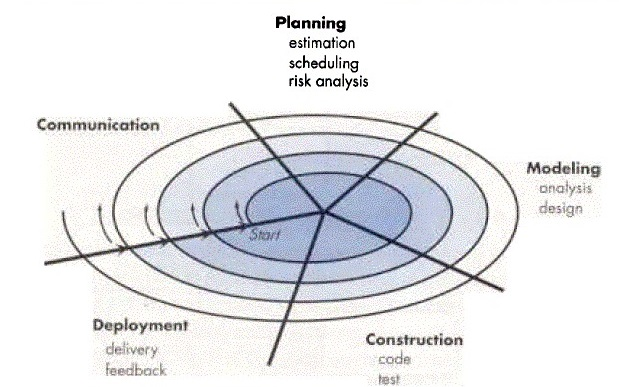
\includegraphics[width=10cm,height=7cm]{gambar/spiral}
	\caption{\textit{Spiral Model}}
	\label{spiral_model}
\end{figure}

Ketika proses pengembangan dimulai, tim rekayasa perangkat lunak bergerak searah jarum mengelilingi spiral tersebut dengan dimulai dari intinya. Lintasan pertama putaran spiral menghasilkan perkembangan dari spesifikasi produk; putaran spiral selanjutnya mungkin dipakai untuk mengembangkan sebuah prototype dan secara progresif mengembangkan versi perangkat lunak yang lebih lengkap \cite{Terjemahan_Pressman}.

\section{\textit{Unified Modeling Language} (UML)} 

Salah satu tahap dalam pengembangan sistem adalah tahap desain dimana pada tahap ini semua informasi kebutuhan pengguna dan analisis sistem dituangkan kedalam suatu desain perangkat lunak. Mendesain suatu produk perangkat lunak salah satunya dapat menggunakan pemodelan berorientasi objek (OOP). Menurut Haviluddin dalam \textit{Jurnal Informatika Mulawarman Vol 6 No. 1 (2011)}, \textit{Unified Modelling Language} merupakan alat perancangan sistem yang berorientasi pada objek. Secara filosofi UML diilhami oleh konsep yang telah ada yaitu konsep permodelan Object Oriented karena konsep ini menganalogikan sistem seperti kehidupan nyata yang didominasi oleh objek dan digambarkan atau dinotasikan dalam simbol-simbol yang cukup spesifik \cite{Haviluddin}.
 
Menurut Ir. M. Farid Azis, M.Kom (2005) berpendapat bahwa UML adalah sekumpulan simbol dan diagram untuk memodelkan perangkat lunak. Desain dalam bentuk simbol dan diagram, kemudian diterjemahkan menjadi kode program. Implementasi kode program dari diagram UML dapat menggunakan bahasa pemrograman apa saja dengan syarat bahasa pemrograman tersebut harus mendukung pemrograman berorientasi objek (OOP) \cite{Azis}. 

Berdasarkan kedua pendapat di atas dapat disimpukan bahwa UML adalah suatu alat yang digunakan untuk memodelkan atau mendesain perangkat lunak dalam bentuk simbol dan diagram dimana sistem dari perangkat lunak tersebut menggunakan pemrograman berorientasi objek (OOP). Jenis UML yang dipergunakan untuk penelitian ini adalah \textit{use case diagram, class diagram}, dan \textit{activity diagram}. 

\subsection{\emph{Use Case Diagram}} 

Menurut Ade Hendini dalam \textit{Jurnal Khatulistiwa Informatika, Vol. IV, No. 2 (2016)}, \textit{Use Case Diagram }merupakan pemodelan untuk kelakuan (\textit{behavior}) sistem informasi yang akan dibuat. \textit{Use case} digunakan untuk mengetahui fungsi apa saja yang ada di dalam sistem informasi dan siapa saja yang berhak menggunakan fungsi-fungsi tersebut \cite{AdeHendini}. Simbol-simbol yang digunakan dalam \textit{Use Case Diagram} yaitu:

%tabel Simbol Use Case Diagram
\begin{table}[H]
	\centering
	\caption{Simbol-simbol \emph{Use Case Diagram}}
	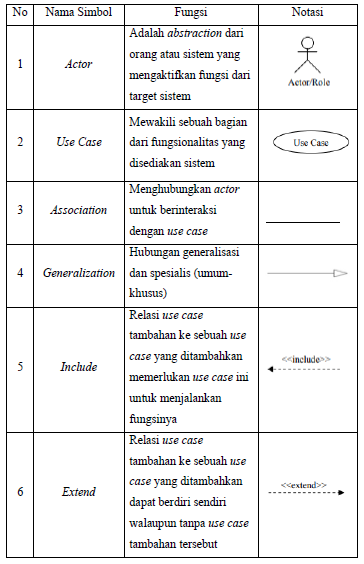
\includegraphics[width=1.0\textwidth]{gambar/simbolusecase}
	\label{tabel_karaktermax2}
\end{table}

\begin{figure}[H]
	\centering
	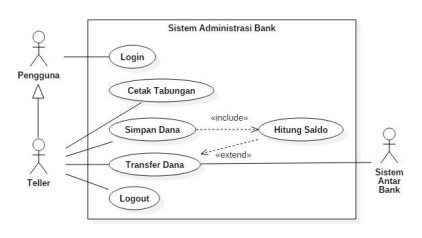
\includegraphics[width=11cm,height=6cm]{gambar/contohusecase}
	\caption{\textit{Contoh \textit{Use Case Diagram}}}
	\label{contoh_usecase}
\end{figure}

\subsection{\emph{Activity Diagram}} 

\emph{Activity Diagram} menggambarkan \textit{workflow} (aliran kerja) atau aktivitas dari sebuah sistem atau proses bisnis \cite{AdeHendini}. Berikut simbol dari activity diagram:

%tabel Simbol Activity Diagram
\begin{table}[H]
	\centering
	\caption{Simbol-simbol \emph{Activity Diagram}}
	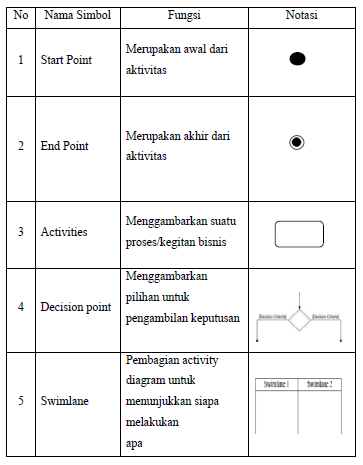
\includegraphics[width=1.0\textwidth]{gambar/simbolactivity}
	\label{tabel_karaktermax2}
\end{table}

\subsection{\emph{Class Diagram}}

\textit{Class diagram} menggambarkan \textit{class} dan hubungan antar-\textit{class} di dalam sisem. 
\textit{Class} digambarkan dengan sebuah kotak dibagi menjadi tiga bagian. Bagian paling atas diisikan nama \textit{class}, 
bagian tengah diisikan variabel yang dimiliki \textit{class} dan bagian bawah diisikan \textit{method} dari \textit{class} \cite{Azis}.

\begin{figure}[H]
	\centering
	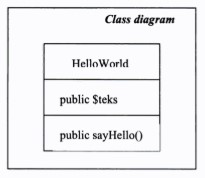
\includegraphics[width=6cm,height=5cm]{gambar/contohclass}
	\caption{\textit{Contoh sederhana \textit{Class Diagram}}}
	\label{contoh_class}
\end{figure}

\textit{Class Diagram} secara khas meliputi: Kelas (\textit{Class}), Relasi Asosiasi/\textit{Associations}, Generalisasi/\textit{Generalization} dan Agregasi/\textit{Aggregation}, atribut (\textit{Attributes}), 
operasi (\textit{operation/method}), dan hubungan antar kelas mempunyai keterangan yang disebut dengan \textit{Multiplicity}
atau \textit{Cardinality}.

\begin{table}[H]
	\centering
	\caption{\emph{Multiplicity Class Diagram}}
	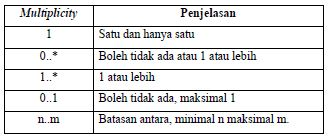
\includegraphics[width=1.0\textwidth]{gambar/multiplicity}
	\label{tabel_karaktermax2}
\end{table}
Berikut simbol-simbol yang terdapat pada class diagram beserta deskripsinya:
\begin{table}[H]
	\centering
	\caption{Simbol-simbol \emph{Class Diagram}}
	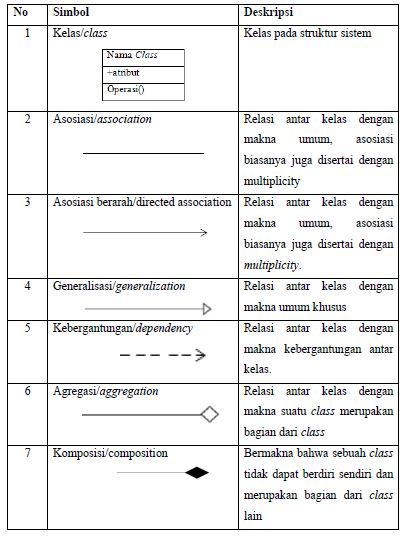
\includegraphics[width=1.0\textwidth]{gambar/simbolclass}
	\label{tabel_karaktermax2}
\end{table}

\section{\emph{Entity Relationship Database}(ERD)}

Komponen utama dari suatu sistem informasi adalah data, data akan diolah menjadi suatu informasi yang digunakan untuk pengambilan keputusan. Salah satu cara dalam memodelkan suatu data ialah dengan menggunakan \textit{Entity Relationship Diagram} (ERD).\textit{ Entity Relationship Diagram} (ERD) adalah sekumpulan cara atau peralatan untuk mendeskripsikan data-data atau objek-objek yang dibuat berdasarkan dan berasal dari dunia nyata yang disebut entitas (\textit{entity}) serta hubungan (\textit{relationship}) antar entitas-entitas tersebut \cite{DoroEdi}. 

Simbol-simbol dalam ERD (\textit{Entity Relationship Diagram}) adalah sebagai berikut \cite{Fridayanthie}.
\begin{enumerate}
	\item Entitas: suatu yang nyata atau abstrak yang mempunyai karakteristik dimana kita akan menyimpan data.
	\item Atribut: ciri umum semua atau sebagian besar instansi pada entitas tertentu.
	\item Relasi: hubungan alamiah yang terjadi antara satu atau lebih entitas. Jenis relasi yang ada pada ERD, yaitu one-to-one, one-to-many, dan many-to-many.
	
\end{enumerate}



\section{\emph{Model View Controller} (MVC)}

MVC merupakan arsitektur yang membagi aplikasi menjadi tiga bagian secara konsep yang terpisah yaitu \textit{Model}, \textit{View}, dan \textit{Controller}, masing-masing dapat dikembangkan secara terpisah antara satu dengan yang lainnya, sehingga perubahan pada satu bagian memiliki dampak minimal pada bagian lain. Bagian model digunakan untuk mendefinisikan suatu cara dimana data dapat diakses, bagian view menghasilkan keluaran jika diberikan data, dan bagian controller menerima perintah dan mengatur aplikasi untuk tugas dan tampilan yang sesuai \cite{AriefHidayat}. 

Untuk lebih jelasnya berikut tiga komponen yang membangun MVC \cite{Wellem} :
\begin{enumerate}
	\item Model, digunakan untuk mengelola informasi atau data dan merepresentasikannya kepada pengguna. Pada umumnya, \textit{Model} berisi fungsi-fungsi yang berhubungan dengan \textit{database}, seperti pengambilan data, \textit{update} data, \textit{insert} data, \textit{delete} data, dan lain sebagainya.
	\item \textit{View}, merupakan informasi yang direpresentasikan kepada pengguna. \textit{View} biasanya berupa halaman web, dimana pengguna dapat melihat informasi yang ditampilkan.
	\item \textit{Controller}, memberikan pelayanan yang menjembatani \textit{Model} dan \textit{View}. \textit{Controller} berisi fungsi-fungsi yang dapat membantu menjembatani \textit{Model} dan \textit{View}. Request datang dan di-\textit{response} melalui \textit{Controller}, kemudian \textit{Controller} berkomunikasi serta melakukan kontrol terhadap \textit{View} dan \textit{Model}.
\end{enumerate}

\begin{figure}[H]
	\centering
	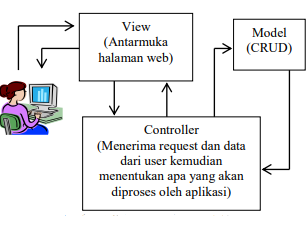
\includegraphics[width=7cm,height=5cm]{gambar/alurmvc}
	\caption{Alur Kerja MVC}
	\label{alurmvc}
\end{figure}

MVC dimulai pada saat pengguna memulai mengakses aplikasi. Awalnya pengguna akan menjalankan operasi pada bagian \textit{View}. Proses ini dapat berupa proses\textit{ Login}, Pendaftaran ataupun proses lainnya. Kemudian perintah akan direspon oleh bagian \textit{Controller}. Bagian\textit{ Controller} akan menentukan apakah permintaan dari pengguna akan diproses atau tidak, ketika diproses maka permintaan akan diarahkan ke bagian\textit{ Model}. Setelah permintaan dari pengguna dapat dipenuhi oleh \textit{model} maka informasi akan dikirimkan kembali ke bagian \textit{controller} lalu diberikan ke bagian \textit{view} sehingga pengguna dapat memperoleh informasi sesuai yang diinginkan \cite{Martono}.

\section{Basis Data} 

Basis data terdiri dari dua kata, yaitu basis dan data. Basis dapat diartikan sebagai markas, gudang, dan tempat berkumpul. Sedangkan data adalah fakta yang mewakili suatu objek seperti manusia, barang hewan, peristiwa dan sebagainya, yang direkam dalam bentuk angka, huruf, simbol, teks, gambar, bunyi atau kombinasinya. Menurut Robi Yanto, M.Kom basis data dapat didefinisikan sebagai himpunan kelompok data yang saling berhubungan yang diorganisasi sedemikian rupa agar dapat dimanfaatkan kembali dengan cepat dan mudah \cite{Robi}. 

Sedangkan menurut Edhy Sutanta basis data dapat dipahami sebagai suatu kumpulan data terhubung (\textit{interrelatet data}) yang disimpan secara bersama-sama pada suatu media, data disimpan dengan cara-cara tertentu sehingga mudah untuk digunakan atau ditampilkan kembali; data dapat digunakan oleh satu atau lebih program-program aplikasi secara optimal; data disimpan sedemikian rupa sehingga proses penambahan, pengambilan, dan modifikasi data dapat dilakukan dengan mudah dan terkontrol \cite{Edhy}. 

Berdasarkan dari kedua pendapat tersebut, basis data dapat dikatakan merupakan sekumpulan kelompok data yang saling terhubung satu sama lain, disimpan dan diatur sedemikian rupa pada suatu media agar data dapat diambil dan dikelola dengan mudah. 

Sistem adalah sekumpulan komponen-komponen yang saling berhubungan dan secara bersama-sama bertujuan untuk memenuhi suatu pekerjaan tertentu. Komponen penting dalam sistem basis data adalah \cite{Robi}:

\begin{enumerate}
	\item Data
	
	Merupakan informasi yang disimpan dalam suatu struktur tertentu yang terintegrasi
	\item \textit{Hardware}
	
	Merupakan perangkat keras berupa komputer dengan media penyimpanan data karena pada umumnya basis data memiliki ukuran yang besar
	\item Sistem Operasi
	
	Program yang mengaktifkan dan memfungsikan sistem komputer, mengendalikan seluruh sumber daya dalam komputer, dan melakukan operasi dasar dalam komputer meliputi input, proses, dan output. 
	\item Basis Data
	
	Sebagai inti dari sistem basis data. Basis data menyimpan data serta struktur sistem basis data baik untuk entitas maupun objek-objek secara detail.
	\item \textit{Database Management System}
	
	Merupakan perangkat lunak yang digunakan untuk melakukan pengelolaan basis data sebagai contoh \textit{Microsoft access, Sql Server, Mysql}, dan \textit{Oracle}. 
	\item \textit{User}
	
	Merupakan pengguna yang menggunakan data yang tersimpan dan terkelola. \textit{User} dapat berupa seseorang yang mengelola basis data yang disebut database administrator (DBA), bisa juga disebut \textit{end user}. 
\end{enumerate}

Basis data dapat digolongkan berdasarkan beberapa kriteria, salah satunya ialah berdasarkan seberapa sering basis data mengalami perubahan dikenal dua penkategorian yaitu \cite{Sulianta} :

\begin{enumerate}
	\item Tabel/data master adalah tabel yang datanya cenderung jarang berubah dan tidak memiliki ketergantungan dengan tabel lain.
	\item Tabel/data transaksi adalah tabel yang datanya sering berubah dan membutuhkan data master untuk membangun komponennya 
\end{enumerate}

		
% Baris ini digunakan untuk membantu dalam melakukan sitasi
% Karena diapit dengan comment, maka baris ini akan diabaikan
% oleh compiler LaTeX.
\begin{comment}
bibliography{daftar-pustaka}
\end{comment}


%!TEX root = ./template-skripsi.tex
%-------------------------------------------------------------------------------
%                            BAB III
%               			PEMBAHASAN
%-------------------------------------------------------------------------------

\chapter{IMPLEMENTASI PROGRAM}

Secara umum tahapan pengembangan sistem dalam metode \emph{System Development Life Cycle} (SDLC) adalah analisis kebutuhan perangkat lunak, desain sistem, konstruksi atau pengembangan, dan pengujian atau evaluasi.


\section{Analisis Kebutuhan}

Kebutuhan mengenai sistem didapat berdasarkan hasil analisis perbandingan sistem \textit{tracer study} yang sudah ada yaitu, Sistem \textit{Tracer Study} Dikti, dan Sistem Informasi \textit{Tracer Study} Universitas Negeri Jakarta [Lampiran A]. Selain itu, melalui pengumpulan data yang diperoleh dari analisis kebutuhan prodi Ilmu Komputer [Lampiran C]. Berikut beberapa kebutuhan yang didapat:
\begin{enumerate}
	\item Memiliki lima pengguna, yaitu admin, koorprodi, alumni, dan pengunjung yang memiliki sub-aktor pengguna alumni. 
	\item Admin dapat mengelola data alumni dan pengguna alumni, membuat kuesioner, menyunting konten beranda, dan menampilkan hasil \textit{tracer study}
	\item Koorprodi dapat menampilkan data alumni dan pengguna alumni, dan dapat menampilkan hasil \textit{tracer study}
	\item Alumni dapat mengelola data diri, riwayat pekerjaan dan mengisi kuesioner yang telah dibuat oleh admin
	\item Pengunjung dapat melakukan pencarian alumni, melihat daftar pengguna alumni, dan melihat data hasil \textit{tracer}. 
	\item Pengguna alumni dapat mengisi form kuesioner.
\end{enumerate}

\section{Desain Sistem}

Pada tahap ini perancangan dan pemodelan sistem dituangkan dalam bentuk visual mulai dari \textit{Use Case Diagram, Activity Diagram, Class Diagram, Entity Relationship Diagram} dan \textit{mock-up} atau rancangan dari tampilan sistem. 

\subsection{\emph{Use Case Diagram}}
\textit{Use Case} digunakan untuk mengetahui fungsi apa saja yang terdapat di dalam suatu sistem dan siapa saja yang berhak menggunakan fungsi-fungsi tersebut. Pada sistem ini terdapat lima aktor yaitu admin, koorprodi, alumni, dan penunjung yang memiliki sub-aktor pengguna alumni. Peran-peran aktor tersebut adalah sebagai berikut:
\begin{enumerate}
	\item Admin
	\begin{itemize}
		\item Admin dapat mengelola data alumni
		\item Admin dapat mengelola data pengguna alumni
		\item Admin dapat membuat form kuesioner \textit{tracer study}
		\item Admin dapat menyunting kata pengantar \textit{tracer study}
		\item Admin dapat melihat laporan/hasil \textit{tracer study} 
	\end{itemize}
	\item Koorprodi 
	\begin{itemize}
		\item Koorprodi dapat melihat data alumni
		\item Koorprodi dapat melihat data pengguna alumni
		\item Koorprodi dapat melihat hasil \textit{tracer study}
	\end{itemize} 
	\item Alumni
	\begin{itemize}
		\item Alumni dapat mengelola data diri dan riwayat pekerjaan
		\item Alumni dapat mengisi form kuesioner \textit{tracer study}
		\item Alumni dapat melihat daftar pengguna alumni serta alumni yang bekerja
	\end{itemize}
	\item Pengunjung
	\begin{itemize}
		\item Pengunjung dapat melihat daftar alumni
		\item Pengunjung dapat melihat daftar pengguna alumni
		\item Pengunjung dapat melihat data \textit{tracer}
	\end{itemize}
	\item Pengguna Alumni
	\begin{itemize}
		\item Pengguna Alumni dapat mengisi form kuesioner
	\end{itemize}
\end{enumerate}

Berikut adalah \textit{Use Case Diagram} dari Sistem Informasi \textit{Tracer Study} Ilmu Komputer FMIPA UNJ

\begin{figure}[H]
	\centering
	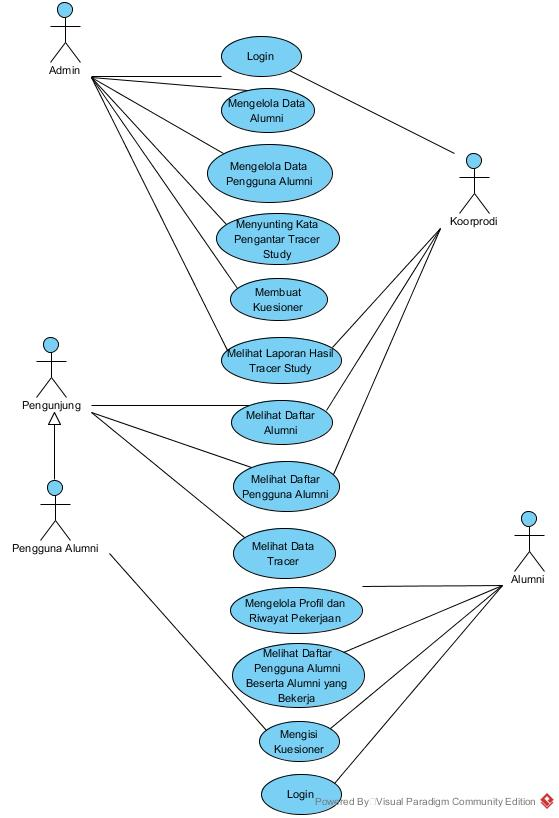
\includegraphics[width=1.0\textwidth]{gambar/usecase}
	\caption{\emph{Use Case Diagram} Sistem Informasi \textit{Tracer Study} Ilmu Komputer}
	\label{usecase_diagram}
\end{figure}


\subsection{\emph{Entity Relationship Diagram}}

ERD dibawah ini menggambarkan masing-masing entitas dan relasi antar entitas untuk basis data Sistem Informasi \textit{Tracer Study} Ilmu Komputer yang akan menyimpan data yang dibutuhkan sistem di antaranya data alumni, pengguna alumni, kuesioner dan hasil kuesioner. Pada ERD ini dibuat tabel pekerjaan dimana berfungsi untuk menampung data riwayat pekerjaan setiap alumni dan tabel instansi untuk menyimpan perusahaan-perusahaan tempat alumni bekerja. Kedua tabel tersebut berelasi dengan tabel alumni dan pengguna alumni. Tabel kuesioner berfungsi untuk menampung kuesioner baik kuesioner alumni maupun pengguna alumni dan berelasi dengan tabel pertanyaan untuk menyimpan pertanyaan-pertanyaan kuesioner. Selain itu disediakan tabel jawaban untuk menampung jawaban kuesioner. Berikut pemodelan ERD sistem informasi \textit{Tracer Study} Ilmu Komputer. 

\begin{figure}[H]
	\centering
	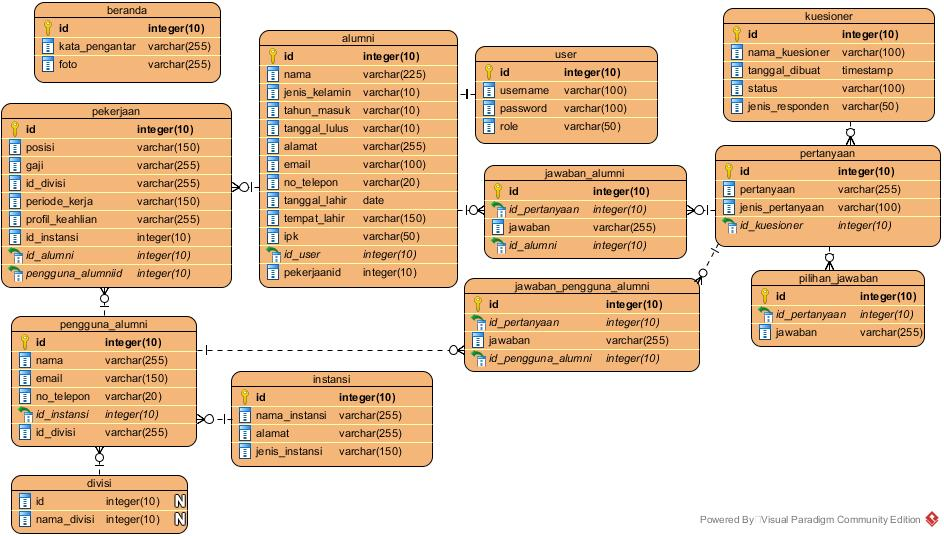
\includegraphics[width=1.0\textwidth]{gambar/erd}
	\caption{\emph{Entity Relationship Diagram} Sistem Informasi \textit{Tracer Study} Ilmu Komputer}
	\label{entityrelationship_diagram}
\end{figure}

\subsection{\textit{Class Diagram}}

Pemodelan \textit{Class Diagram} pada Sistem Informasi \textit{Tracer Study} Ilmu Komputer memiliki sembilan \textit{Class}. Terdapat \textit{Class user} yang menyimpan metode \textit{login, logout,} dan mengganti \textit{password}. \textit{Class} ini memiliki tiga \textit{subclass} dimana dapat mengakses metode dan atribut dari\textit{ Class} tersebut yaitu admin, koorprodi, dan alumni.\textit{ Class} kuesioner untuk menampung kuesioner dan berelasi dengan \textit{Class} pertanyaan yang berisi metode untuk mengelola pertanyaan kuesioner. Selanjutnya terdapat \textit{Class} hasil berfungsi untuk mengelola dan menampilkan hasil kuesioner dan \textit{Class} pekerjaan untuk mengelola data pekerjaan alumni. Berikut adalah \textit{Class Diagram} dari sistem Informasi \textit{Tracer Study} Ilmu Komputer

\begin{figure}[H]
	\centering
	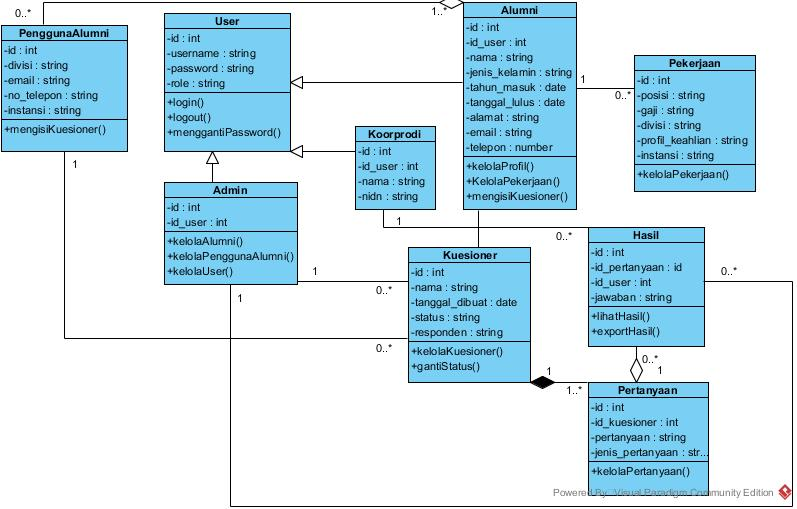
\includegraphics[width=1.0\textwidth]{gambar/class}
	\caption{Desain \emph{Class Diagram} Sistem Informasi \textit{Tracer Study} Ilmu Komputer}
	\label{class_diagram}
\end{figure}


\subsection{\textit{Activity Diagram}}

Desain \textit{Activity Diagram} pada sistem ini dibagi menjadi lima diagram, yaitu membuat form kuesioner untuk admin, melihat hasil atau laporan \textit{tracer study} untuk admin dan koorprodi, mengisi riwayat pekerjaan untuk alumni dan mengisi form kuesioner untuk alumni dan pengguna alumni. Berikut ini \textit{Activity Diagram} dari Sistem Informasi \textit{Tracer Study} Ilmu Komputer

\begin{figure}[H]
	\centering
	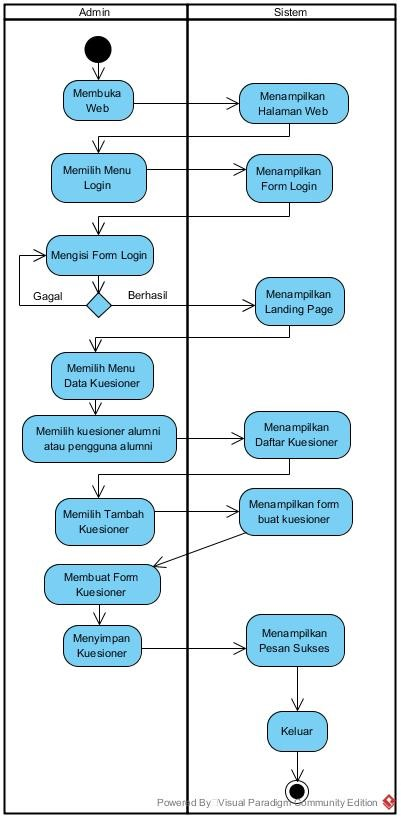
\includegraphics[width=8cm,height=15cm]{gambar/Activitykelolakuesioner}
	\caption{\emph{Activity Diagram} Membuat Kuesioner \textit{Tracer Study}}
	\label{activity_kelolakuesioner}
\end{figure}

Gambar 3.4 menggambarkan aktivitas dalam membuat form kuesioner baik untuk kuesioner alumni maupun pengguna alumni yang dilakukan oleh admin. Dalam pembuatan form kuesioner, admin dapat menambahkan pertanyaan kuesioner dimana disediakan empat jenis pertanyaan, yaitu pertanyaan isian, pilihan, pilihan ganda, dan pertanyaan dengan jawaban skala.  

\begin{figure}[H]
	\centering
	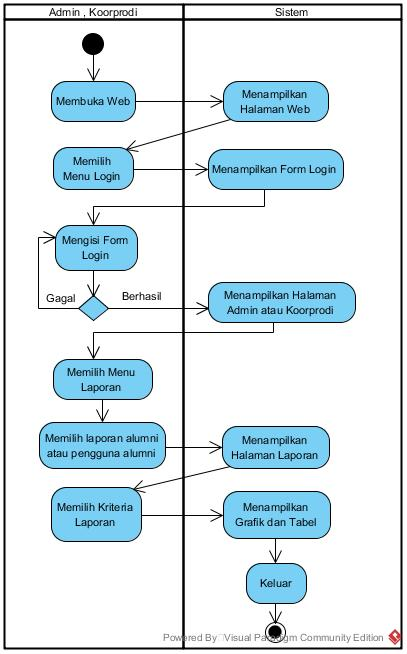
\includegraphics[width=9cm,height=15cm]{gambar/Activitymelihatlaporan}
	\caption{\emph{Activity Diagram} Melihat Laporan \textit{Tracer Study}}
	\label{activity_melihatlaporan}
\end{figure}

Pada \textit{Activity Diagram} melihat laporan, admin dan koorprodi dapat melihat laporan hasil \textit{tracer study} baik alumni dan pengguna alumni. Sebelum menampilkan laporan, admin dan koorprodi mengisi kriteria yang dipilih yaitu berdasarkan jenis kuesioner, pertanyaan yang ingin dilihat hasilnya, dan juga tahun lulus, kemudian sistem akan menampilkan hasil \textit{tracer study} dalam bentuk grafik dan tabel. Selain itu, pada halaman hasil \textit{tracer study} admin dan koorprodi dapat mengekspor data \textit{tracer} dalam format \textit{excel}. 
%kemungkinan halaman laporan berubah

\begin{figure}[H]
	\centering
	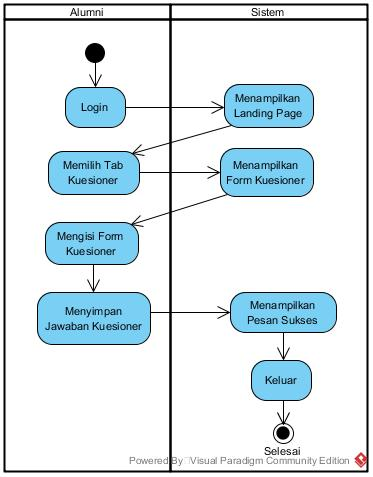
\includegraphics[width=10cm,height=12cm]{gambar/Activitykuesioneralumni}
	\caption{\emph{Activity Diagram} Mengisi Kuesioner Alumni}
	\label{activity_kuesioneralumni}
\end{figure}

Gambar 3.6 menjelaskan aktivitas mengisi kuesioner yang dilakukan oleh alumni. Pada sistem ini juga disediakan form riwayat pekerjaan agar terlihat rekam jejak dari setiap pekerjaan alumni yang pernah digeluti dan juga untuk mengisi data mengenai pengguna alumni. Desain tampilan dari aktivitas mengisi riwayat pekerjaan untuk alumni sebagai berikut.

\begin{figure}[H]
	\centering
	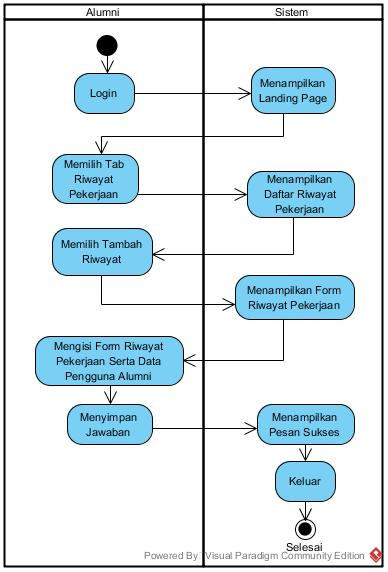
\includegraphics[width=10cm,height=15cm]{gambar/Activityriwayatpekerjaan}
	\caption{\emph{Activity Diagram} Mengisi Riwayat Pekerjaan Alumni}
	\label{activity_pekerjaanalumni}
\end{figure}

Pada sistem \textit{tracer study} ini pengguna alumni juga dapat mengisi kuesioner. Alur dari aktivitas pengisian kuesioner oleh pengguna alumni dapat dilihat pada gambar berikut.

\begin{figure}[H]
	\centering
	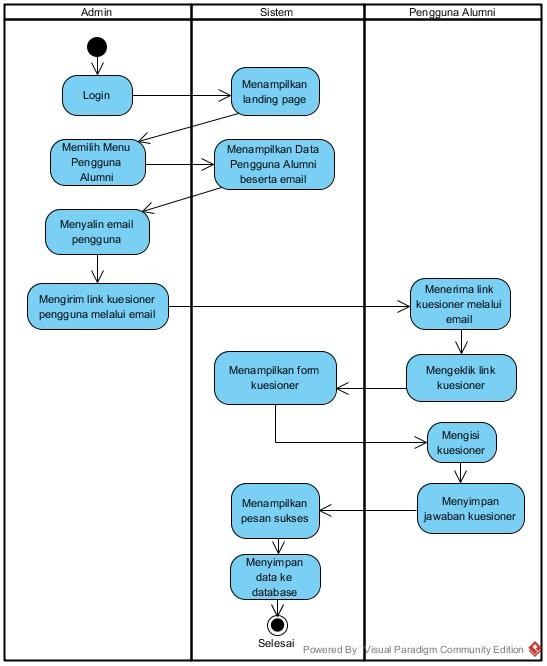
\includegraphics[width=12cm,height=14cm]{gambar/Activitykuesionerpengguna}
	\caption{\emph{Activity Diagram} Mengisi Kuesioner Pengguna Alumni}
	\label{activity_kuesionerpengguna}
\end{figure}

\begin{figure}[H]
	\centering
	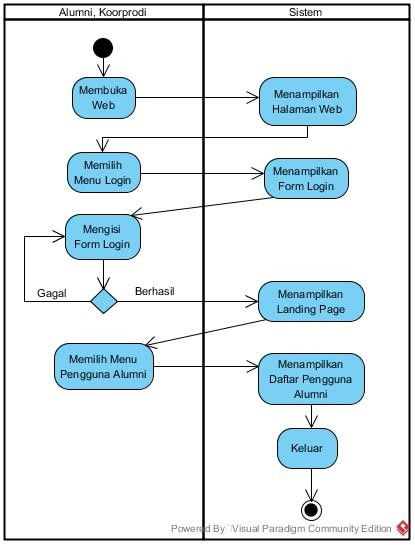
\includegraphics[width=10cm,height=11cm]{gambar/Activitymelihatpengguna}
	\caption{\emph{Activity Diagram} Melihat Daftar Pengguna Alumni}
	\label{activity_kuesionerpengguna}
\end{figure}

Alumni dan koorprodi dapat melihat daftar pengguna alumni, alur dari aktivitas tersebut dapat dilihat pada diagram di atas. Alumni dan koorprodi juga dapat melihat siapa saja alumni yang bekerja pada setiap pengguna alumni. 

\subsection{Rancangan Antar Muka Program}

Rancangan antar muka atau desain tampilan sistem dapat disebut sebagai \textit{mock-up}. Tampilan awal sistem akan memampilkan halaman pengunjung dimana disediakan menu daftar pengguna alumni dan statistik alumni. Di bawah ini adalah \textit{mock-up} untuk tampilan daftar pengguna alumni dimana pengunjung dapat melihat daftar pengguna alumni Ilmu Komputer beserta posisi alumni yang bekerja di intansi tersebut. 

\begin{figure}[H]
	\centering
	\fbox{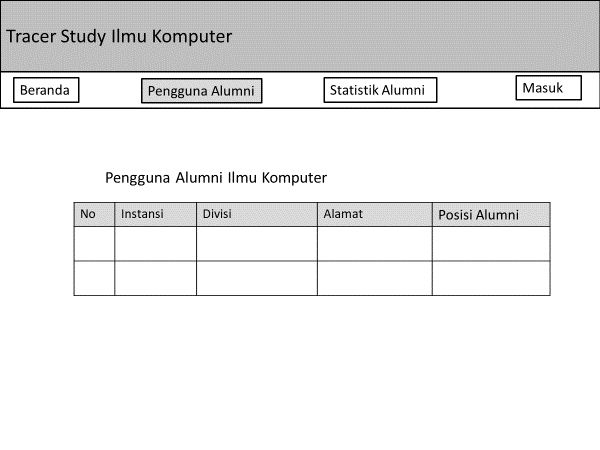
\includegraphics[width=12cm,height=10cm]{gambar/mockup/pengunjung_daftarpengguna}}
	\caption{Desain Halaman Daftar Pengguna Alumni untuk Pengunjung}
	\label{pengunjung_daftarpengguna}
\end{figure}

Sistem juga menyediakan halaman statistik alumni untuk menampilkan data \textit{tracer} yang dapat dilihat oleh pengunjung. Rancangan dari tampilan halaman tersebut dapat dilihat di bawah ini.

\begin{figure}[H]
	\centering
	\fbox{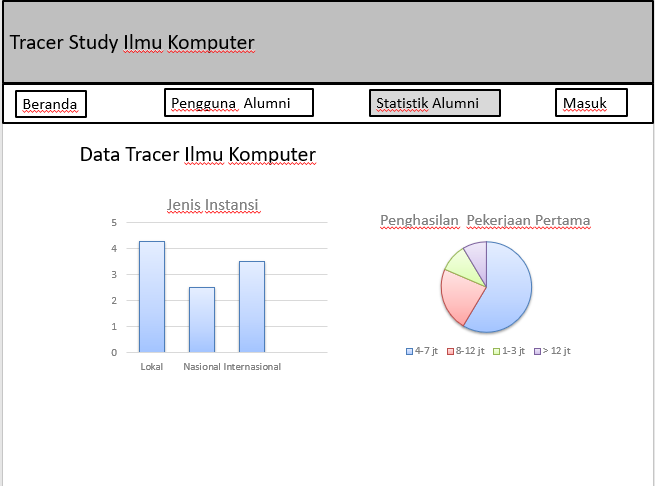
\includegraphics[width=12cm,height=9cm]{gambar/mockup/pengunjung_statistik}}
	\caption{Desain Halaman Statistik Alumni untuk Pengunjung}
	\label{pengunjung_statistik}
\end{figure}

Di bawah ini adalah rancangan tampilan dari halaman admin. Pada tampilan admin terdapat beberapa menu yaitu, beranda, alumni, pengguna alumni, kuesioner, laporan, kelola beranda, dan ganti \textit{password}. 

\begin{figure}[H]
	\centering
	\fbox{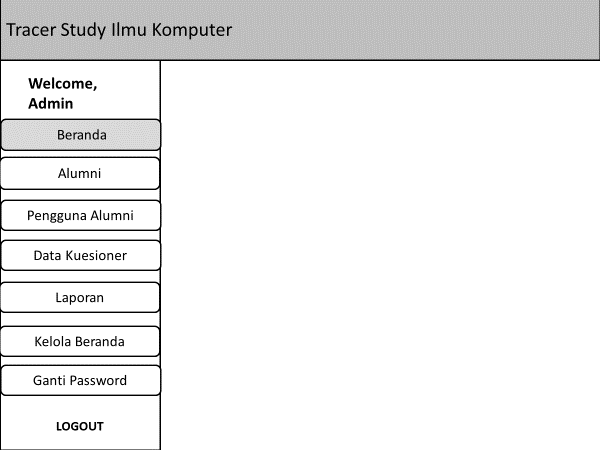
\includegraphics[width=11cm,height=8cm]{gambar/mockup/admin_beranda}}
	\caption{Desain Halaman Admin}
	\label{admin_beranda}
\end{figure}

Admin dapat mengelola data alumni dan pengguna alumni. Berikut ini rancangan tampilan dari kedua halaman tersebut. 

\begin{figure}[H]
	\centering
	\fbox{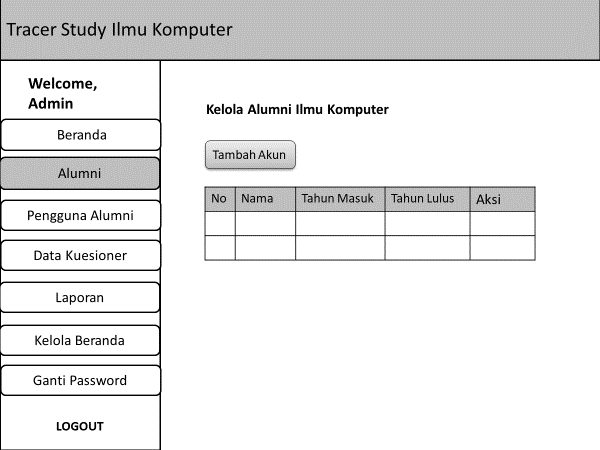
\includegraphics[width=11cm,height=8cm]{gambar/mockup/admin_kelolaalumni}}
	\caption{Desain Halaman Kelola Data Alumni}
	\label{admin_kelolaalumni}
\end{figure}

\begin{figure}[H]
	\centering
	\fbox{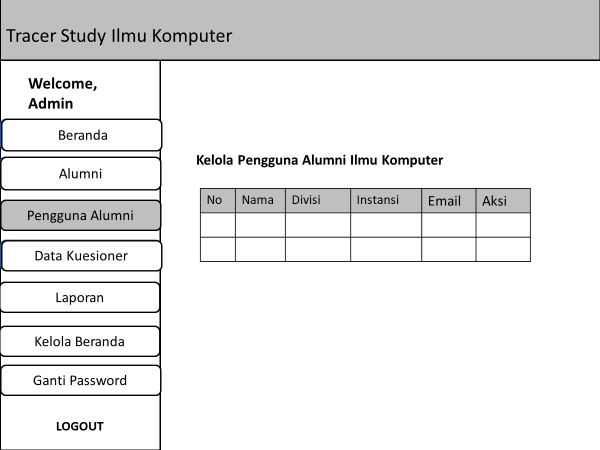
\includegraphics[width=11cm,height=8cm]{gambar/mockup/admin_kelolapengguna}}
	\caption{Desain Halaman Kelola Data Pengguna Alumni}
	\label{admin_kelolapengguna}
\end{figure}

Untuk mengelola kuesioner baik kuesioner alumni dan pengguna alumni dapat dilakukan pada halaman kelola kuesioner dibawah ini. 

\begin{figure}[H]
	\centering
	\fbox{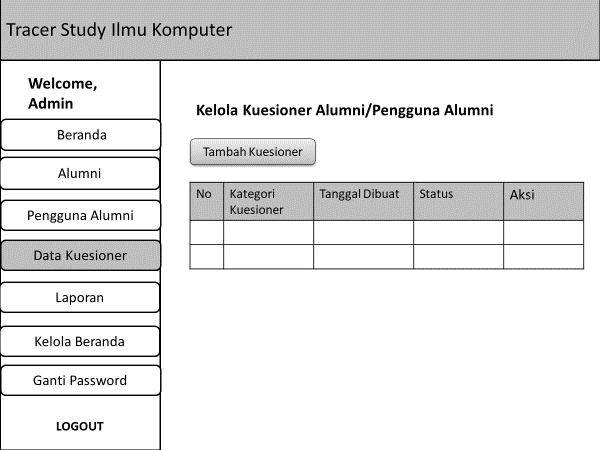
\includegraphics[width=11cm,height=8cm]{gambar/mockup/admin_kelolakuesioner}}
	\caption{Desain Halaman Kelola Kuesioner}
	\label{admin_kelolakuesioner}
\end{figure}

Gambar dibawah merupakan \textit{mock-up} dari tampilan halaman laporan tracer study. Pada halaman ini hasil \textit{tracer study} ditampilkan melalui grafik dan tabel.

\begin{figure}[H]
	\centering
	\fbox{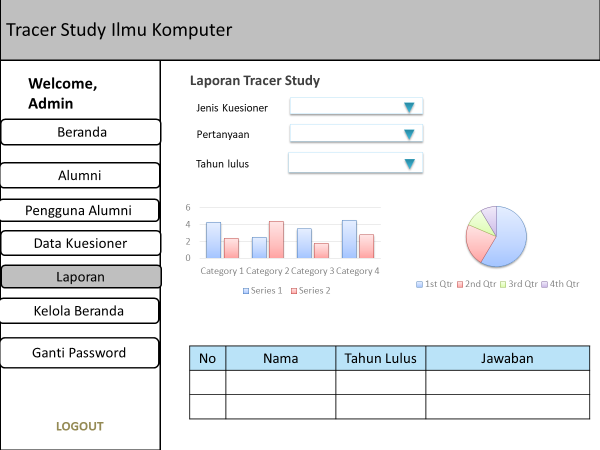
\includegraphics[width=11cm,height=8cm]{gambar/mockup/admin_laporan}}
	\caption{Desain Halaman Laporan \textit{Tracer Study}}
	\label{admin_kelolakuesioner}
\end{figure}

\begin{figure}[H]
	\centering
	\fbox{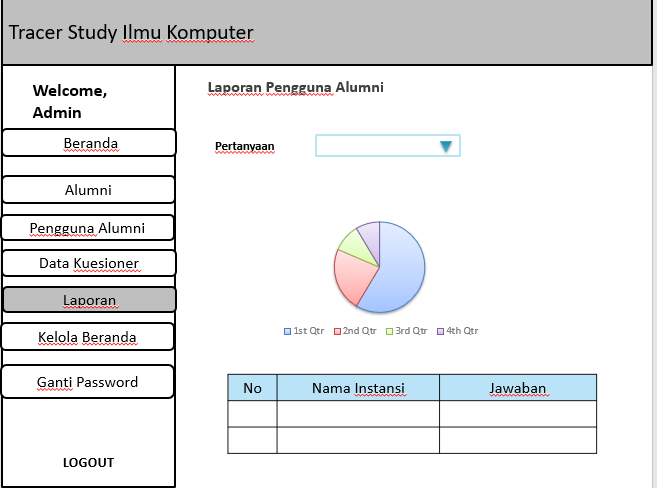
\includegraphics[width=11cm,height=8cm]{gambar/mockup/admin_laporanpengguna}}
	\caption{Desain Halaman Laporan Pengguna Alumni}
	\label{admin_laporanpengguna}
\end{figure}

Pada tampilan koorprodi terdapat beberapa menu, yaitu beranda, alumni, pengguna alumni, laporan, dan ganti password. 

\begin{figure}[H]
	\centering
	\fbox{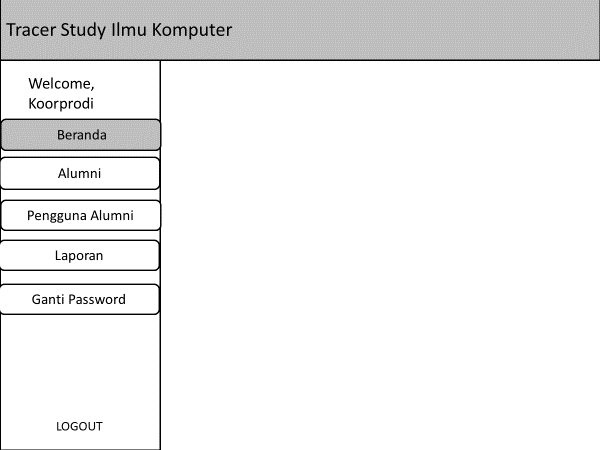
\includegraphics[width=11cm,height=8cm]{gambar/mockup/koorprodi_beranda}}
	\caption{Desain Halaman Koorprodi}
	\label{koorprodi_beranda}
\end{figure}

\begin{figure}[H]
	\centering
	\fbox{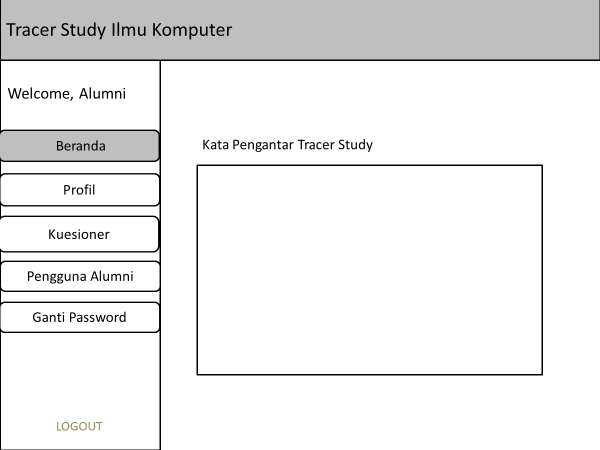
\includegraphics[width=11cm,height=8cm]{gambar/mockup/alumni_beranda}}
	\caption{Desain Halaman Alumni}
	\label{alumni_beranda}
\end{figure}

Selanjutnya beralih ke halaman alumni dimana terdapat beberapa menu, yaitu beranda yang terdiri dari form pengisian data \textit{tracer study} yaitu data diri, pekerjaan dan kuesioner, kemudian menu pengguna alumni, dan menu ganti \textit{password}. Rancangan tampilan halaman alumni dapat dilihat pada gambar 3.19. Alumni dapat mengisi kuesioner melalui halaman kuesioner. Berikut rancangan tampilan dari halaman kuesioner alumni.

\begin{figure}[H]
	\centering
	\fbox{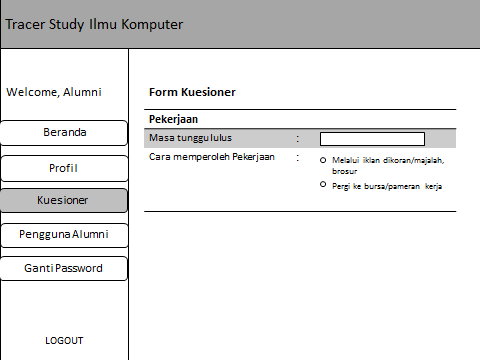
\includegraphics[width=11cm,height=8cm]{gambar/mockup/alumni_kuesioner}}
	\caption{Desain Halaman Kuesioner Alumni}
	\label{alumni_beranda}
\end{figure}

Selanjutnya sistem menyediakan tampilan daftar pengguna alumni yang dapat dilihat alumni beserta siapa saja alumni yang bekerja pada instansi dari pengguna alumni terkait.\textit{ Mock-up} dari tampilan daftar pengguna alumni dapat dilihat sebagai berikut.

\begin{figure}[H]
	\centering
	\fbox{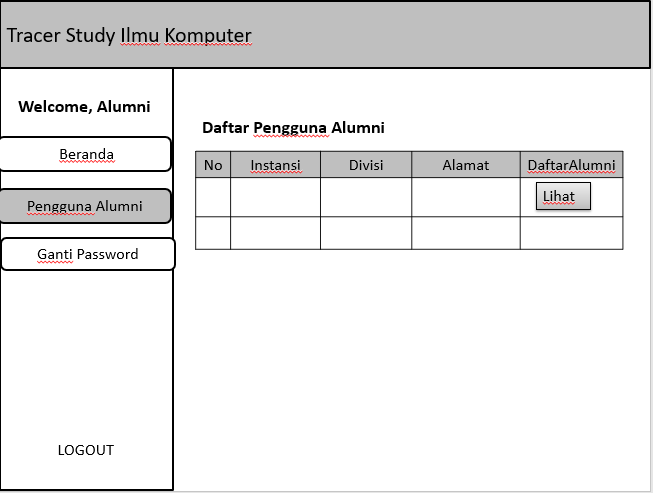
\includegraphics[width=11cm,height=8cm]{gambar/mockup/alumni_daftarpengguna}}
	\caption{Desain Halaman Daftar Pengguna Alumni untuk Alumni}
	\label{alumni_beranda}
\end{figure}

\section{Pengembangan}
Tahap pengembangan atau juga disebut tahap konstruksi merupakan tahapan dimana menuangkan seluruh desain yang telah dibuat kedalam kode program. tahapan ini dimulai dari membangun basis data, mengimplementasikan desain tampilan dan dilanjutkan dengan membangun sistem.  

\subsection{Membangun Basis Data}
Pada tahap ini dibangun basis data berdasarkan \textit{Entity Relationship Diagram} yang dibuat pada tahap sebelumnya, yaitu desain sistem. Basis data dibuat menggunakan MySQL dan memanfaatkan aplikasi phpMyAdmin untuk membuat tabel beserta relasinya. Berikut bentuk basis data Sistem Informasi \textit{Tracer Study} Prodi Ilmu Komputer yang memiliki 12 tabel:

\begin{figure}[H]
	\centering
	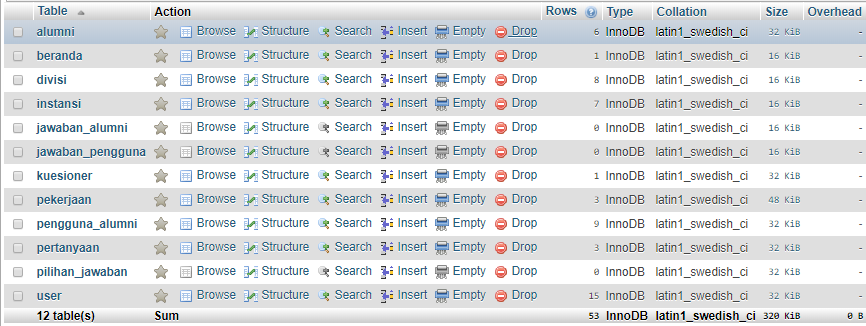
\includegraphics[width=13cm,height=7cm]{gambar/database}
	\caption{Basis Data  Sistem Informasi \textit{Tracer Study} Prodi Ilmu Komputer }
	\label{database}
\end{figure}

\subsection{Implementasi Desain Tampilan}
Untuk mengimplentasikan desain tampilan, digunakan \textit{Bootstrap} sebagai \textit{framework} untuk membuat tampilan atau \textit{front-end} dan CodeIgniter sebagai \textit{framework} untuk \textit{back-end}. Dengan menggunakan CodeIgniter memudahkan dalam mengimplementasikan arsitektur MVC dimana sudah disediakan struktur folder yang sesuai. \textit{Framework Bootsrap} digunakan pada bagian View. Berikut tampilan \textit{website} sistem \textit{tracer study} Ilmu Komputer yang terintegrasi dengan Sistem Informasi Alumni hasil penelitian Ibu Fariani Hermin selaku dosen Ilmu Komputer yang dapat dilihat pada \textit{browser}.

\begin{figure}[H]
	\centering
	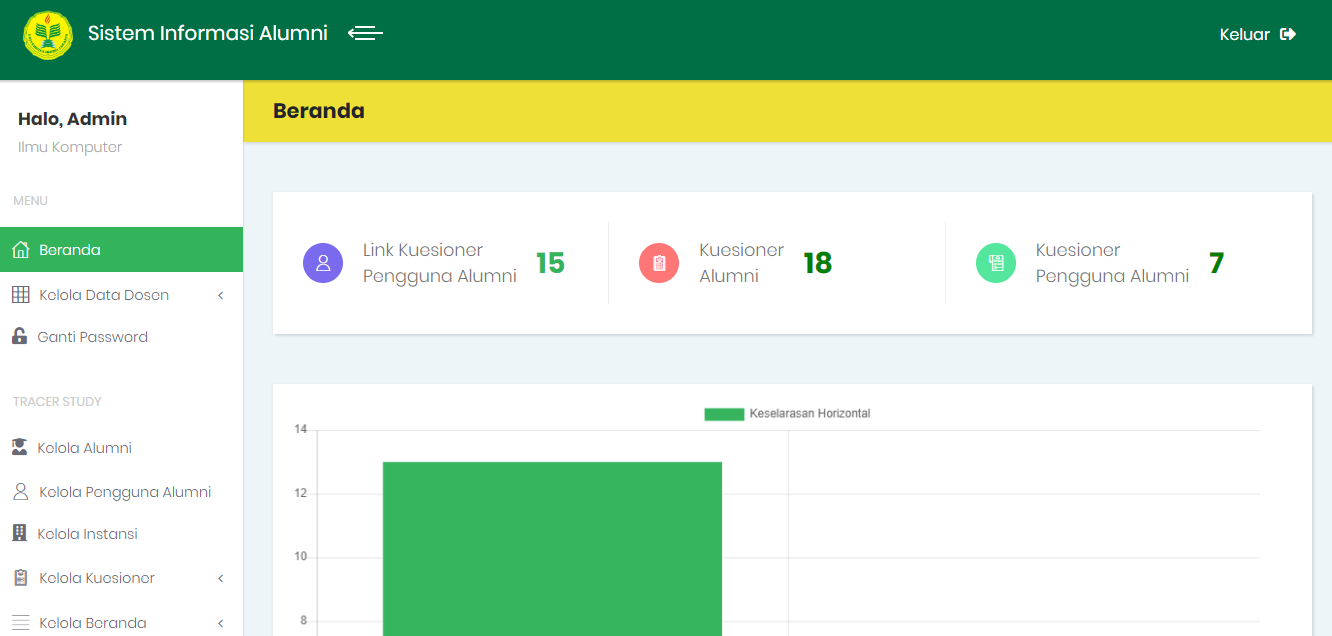
\includegraphics[width=14cm,height=7cm]{gambar/tampilan/admin_beranda}
	\caption{Tampilan Halaman Beranda Admin}
	\label{ui_adminBeranda}
\end{figure}
 
Menu \textit{tracer study} terdapat pada bagian bawah kiri seperti pada Gambar 3.23. Gambar tersebut merupakan tampilan halaman beranda admin yang berisi statistik alumni ilmu komputer, jumlah pengguna alumni yang baru terdaftar, jumlah responden kuesioner alumni dan pengguna alumni. 

\begin{figure}[H]
	\centering
	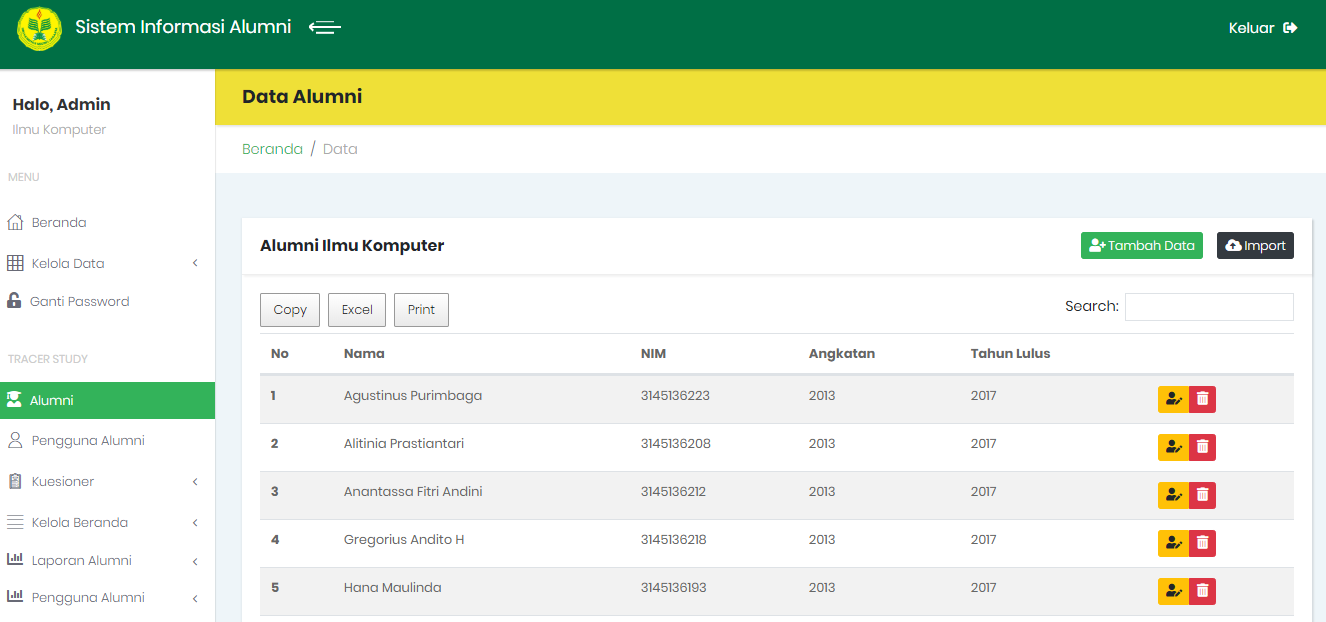
\includegraphics[width=14cm,height=7cm]{gambar/tampilan/admin_kelolaAlumni}
	\caption{Tampilan Halaman Kelola Alumni pada Admin }
	\label{ui_adminKelolaAlumni}
\end{figure}

Gambar 3.24 adalah tampilan pada admin untuk mengelola data alumni seperti tambah, sunting, hapus, dan \textit{import} data alumni.  Selanjutnya, halaman untuk mengelola data pengguna alumni pada admin. Berikut tampilan dari halaman tersebut yang dapat dilihat pada Gambar 3.25.

\begin{figure}[H]
	\centering
	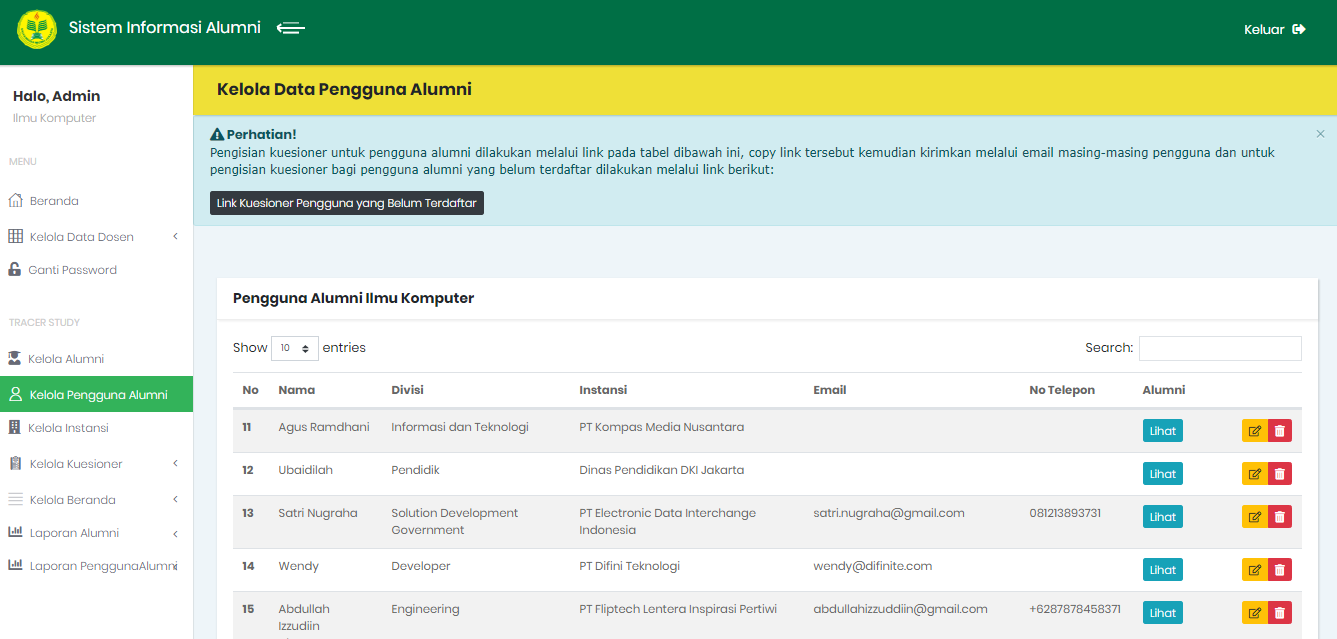
\includegraphics[width=14cm,height=7cm]{gambar/tampilan/admin_kelolaPenggunaAlumni}
	\caption{Tampilan Halaman Kelola Pengguna Alumni pada Admin }
	\label{ui_adminKelolaPenggunaAlumni}
\end{figure}

\begin{figure}[H]
	\centering
	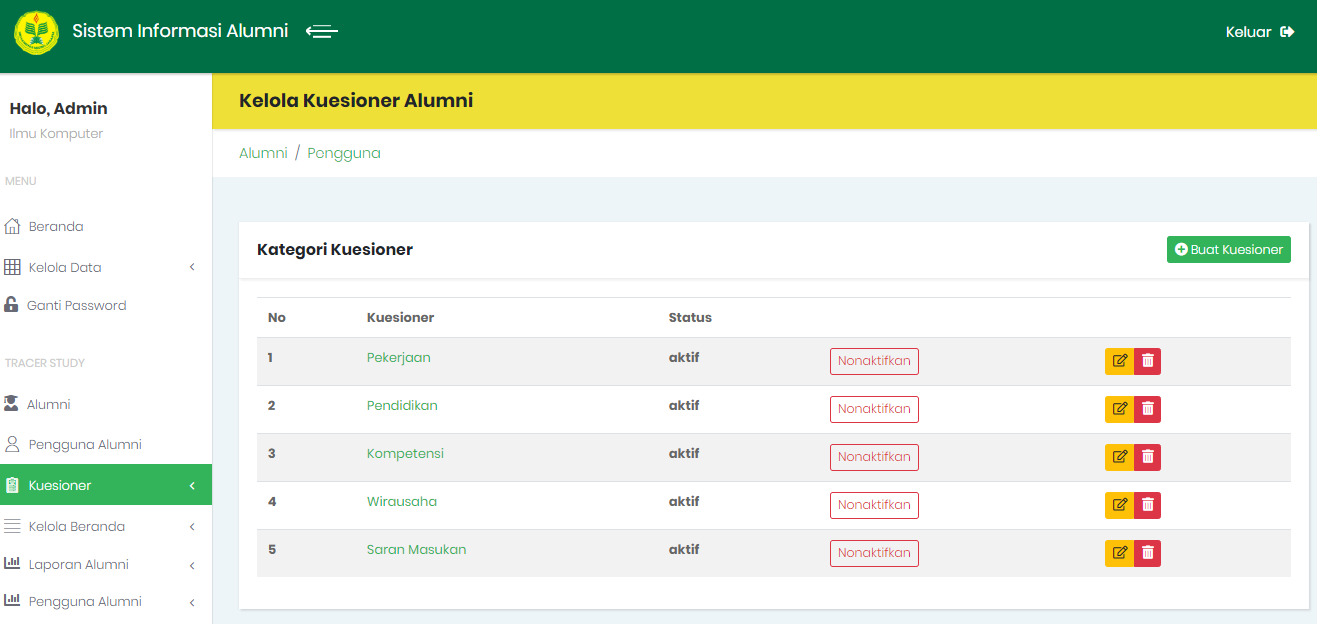
\includegraphics[width=14cm,height=7cm]{gambar/tampilan/admin_kelolaKuesioner}
	\caption{Tampilan Halaman Kelola Kuesioner Alumni pada Admin }
	\label{ui_adminkelolaKuesionerAlumni}
\end{figure}

Gambar 3.26 merupakan tampilan pada admin yang ditujukan untuk mengelola kuesioner-kuesioner alumni. Pada halaman ini tersedia fitur untuk menambah, menyunting, menghapus kuesioner dan dapat mengaktifkan serta menonaktifkan kuesioner. 

\begin{figure}[H]
	\centering
	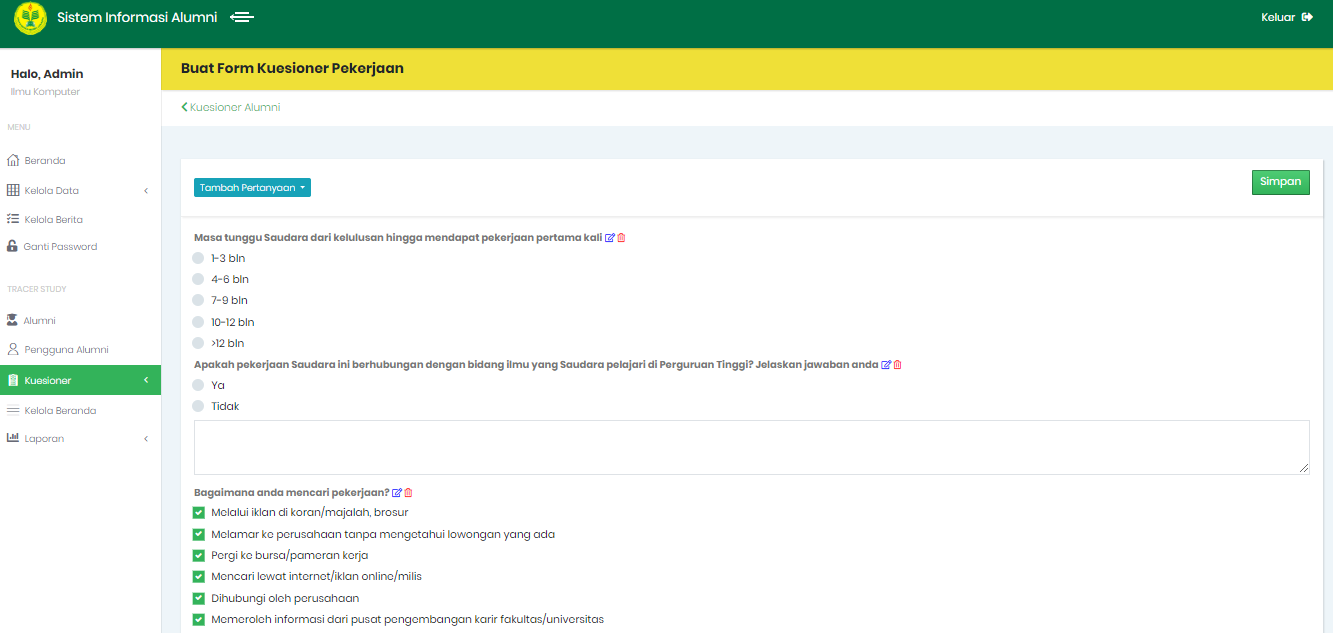
\includegraphics[width=14cm,height=7cm]{gambar/tampilan/admin_buatKuesioner}
	\caption{Tampilan Halaman Buat Kuesioner Alumni pada Admin }
	\label{ui_adminBuatKuesionerAlumni}
\end{figure}

Jika admin memilih tombol buat kuesioner maka sistem akan menampilkan halaman buat kuesioner seperti pada Gambar 3.27. Pada halaman tersebut admin dapat membuat empat jenis pertanyaan, yaitu isian, pertanyaan dengan jawaban pilihan, pertanyaan dengan jawaban lebih dari satu atau ganda, dan pertanyaan dengan jawaban menggunakan skala penilaian.

%penjelasan dan gambar halaman buat kuesioner pengguna
\begin{figure}[H]
	\centering
	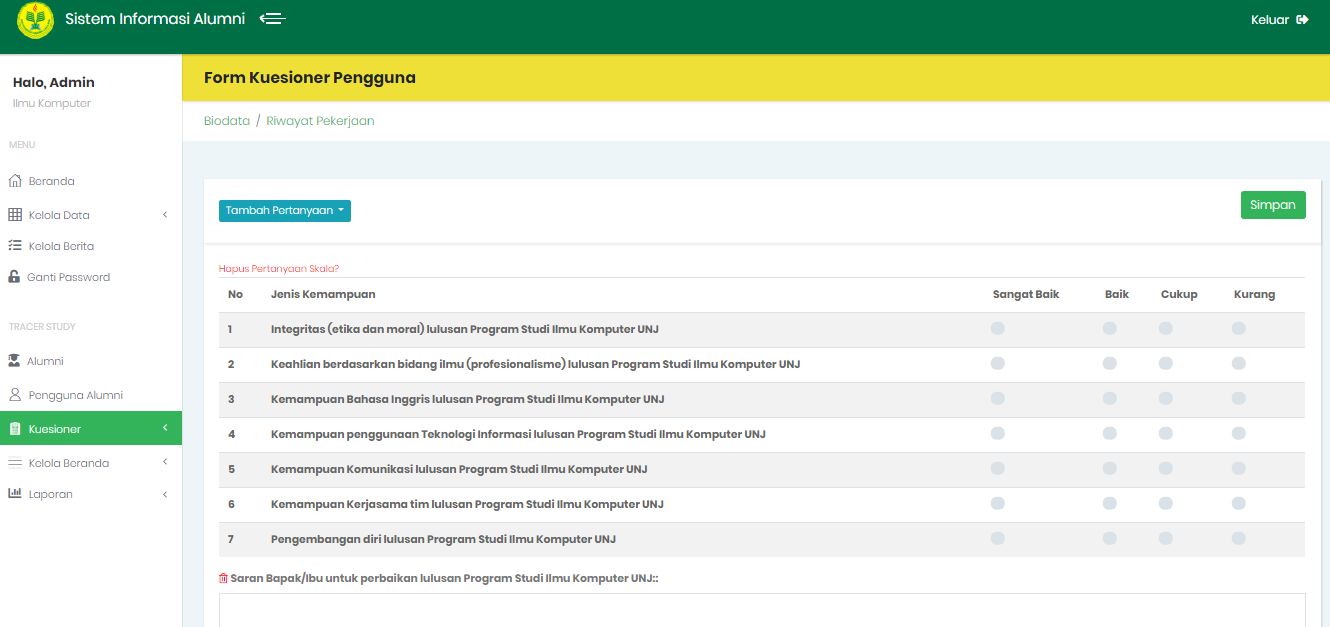
\includegraphics[width=14cm,height=7cm]{gambar/tampilan/admin_buatKuesionerPengguna}
	\caption{Tampilan Halaman Buat Kuesioner Pengguna pada Admin }
	\label{ui_adminBuatKuesionerPenggunaAlumni}
\end{figure}

Selain membuat form kuesioner untuk alumni, admin juga dapat membuat form kuesioner untu pengguna alumni. Tampilan halaman buat form kuesioner pengguna alumni dapat dilihat pada Gambar 3.28. 

\begin{figure}[H]
	\centering
	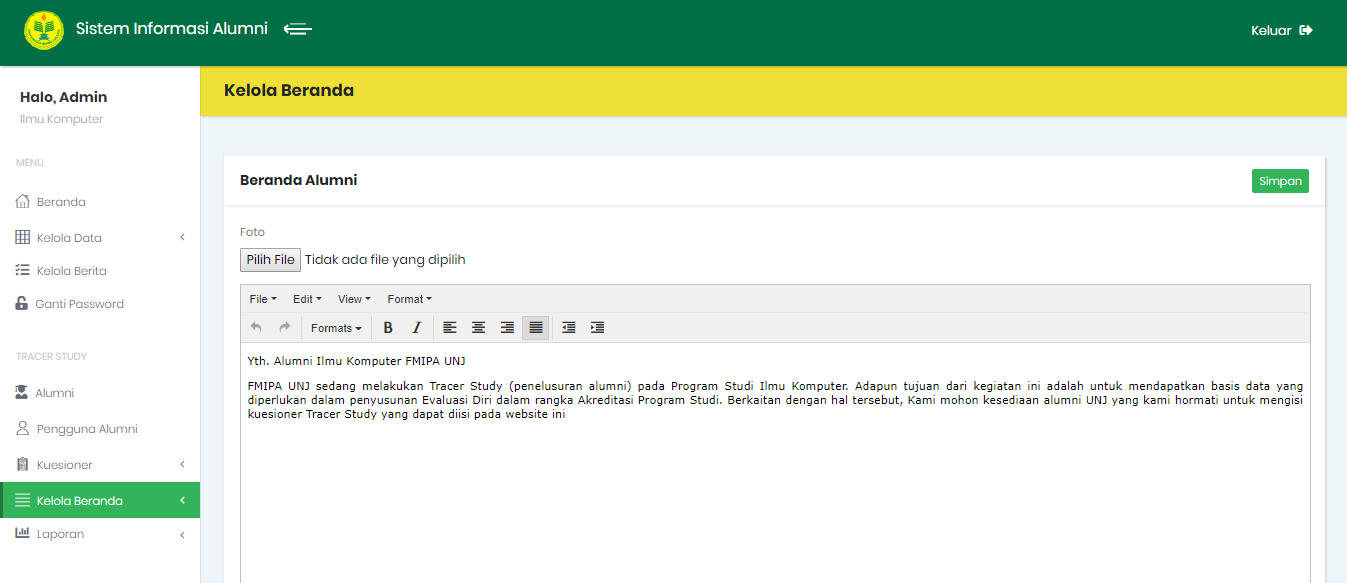
\includegraphics[width=14cm,height=7cm]{gambar/tampilan/admin_kelolaBerandaAlumni}
	\caption{Tampilan Halaman Kelola Beranda Alumni pada Admin }
	\label{ui_adminKelolaBerandaAlumni}
\end{figure}

Pada pengembangan sistem ini juga disediakan fitur untuk mengelola kata pengantar pada beranda alumni agar dapat menyesuaikan jika ada perubahan dari pihak prodi di masa mendatang. Fitur tersebut terdapat pada menu kelola beranda yang tampilannya dapat dilihat pada Gambar 3.29. 

\begin{figure}[H]
	\centering
	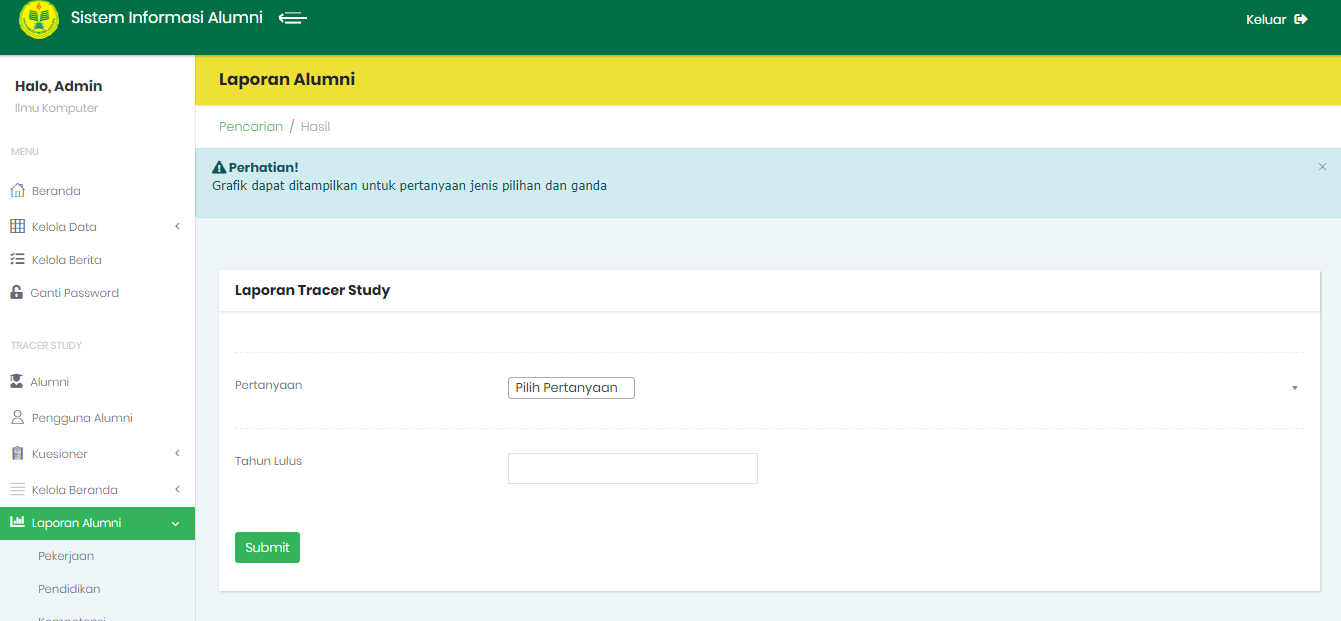
\includegraphics[width=14cm,height=7cm]{gambar/tampilan/admin_cariLaporan}
	\caption{Tampilan Halaman Kriteria Laporan Alumni pada Admin }
	\label{ui_adminCariLaporan}
\end{figure}

\begin{figure}[H]
	\centering
	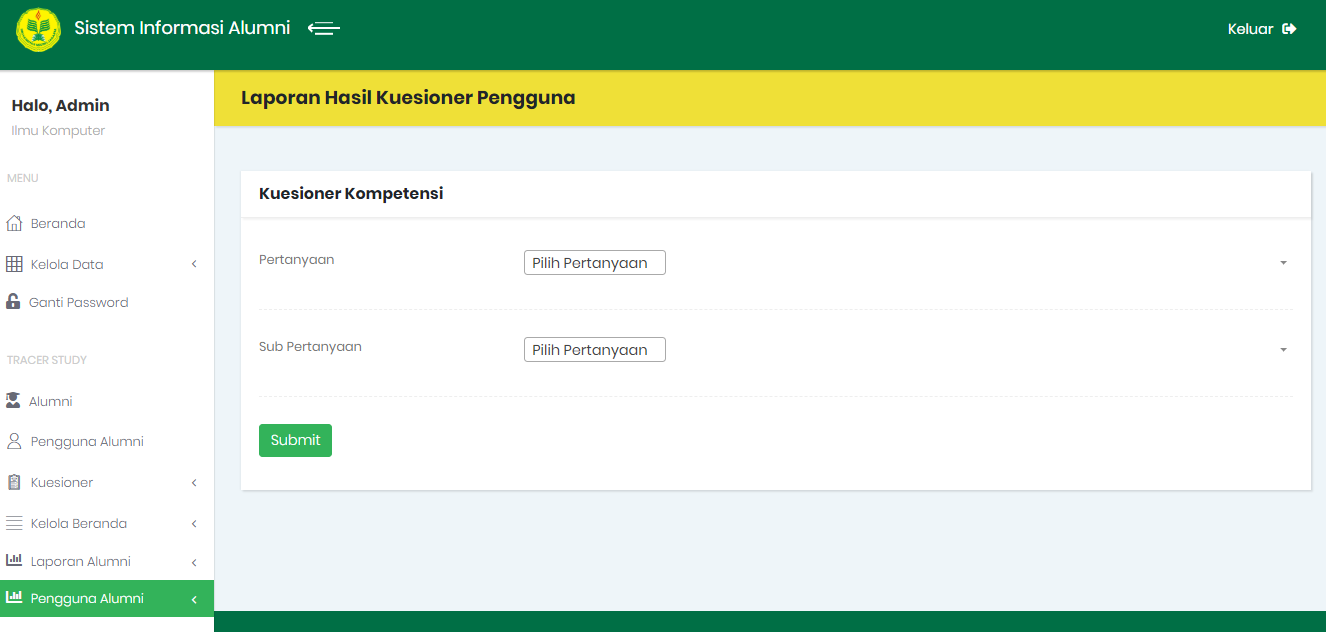
\includegraphics[width=14cm,height=7cm]{gambar/tampilan/admin_cariLaporanPengguna}
	\caption{Tampilan Halaman Kriteria Laporan Pengguna Alumni pada Admin }
	\label{ui_adminCariLaporanPengguna}
\end{figure}

Gambar 3.30 dan Gambar 3.31 merupakan tampilan halaman kriteria laporan atau hasil \textit{tracer study} alumni dan pengguna alumni. Sebelum menampilkan halaman hasil \textit{tracer study}, admin harus memilih terlebih dahulu kriteria laporan yang ingin dilihat, yaitu berupa pertanyaan dan tahun lulus. Setelah admin memilih kriteria maka sistem akan menampilkan halaman hasil \textit{tracer study} berupa grafik dan tabel yang dapat dilihat pada gambar berikut. 

%gambar hasil tracer study Gambar 3.32

\begin{figure}[H]
	\centering
	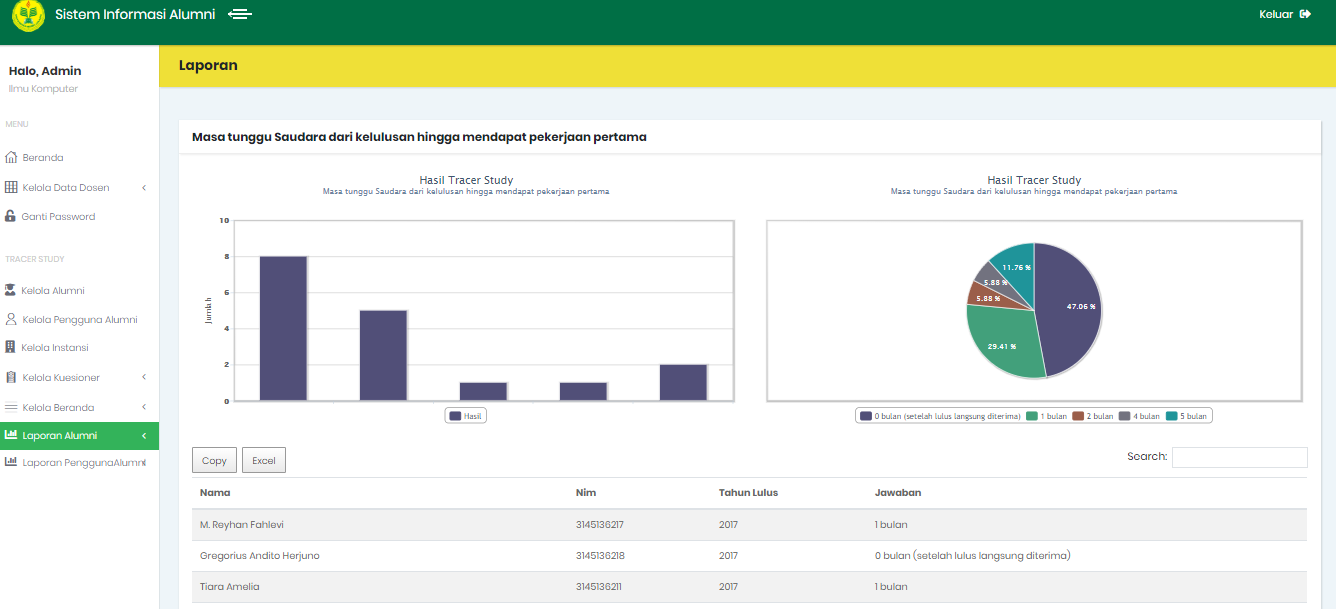
\includegraphics[width=14cm,height=7cm]{gambar/tampilan/admin_hasilLaporanAlumni}
	\caption{Tampilan Halaman Hasil \textit{Tracer Study} pada Admin dan Koorprodi}
	\label{ui_adminHasilLaporanAlumni}
\end{figure}

\begin{figure}[H]
	\centering
	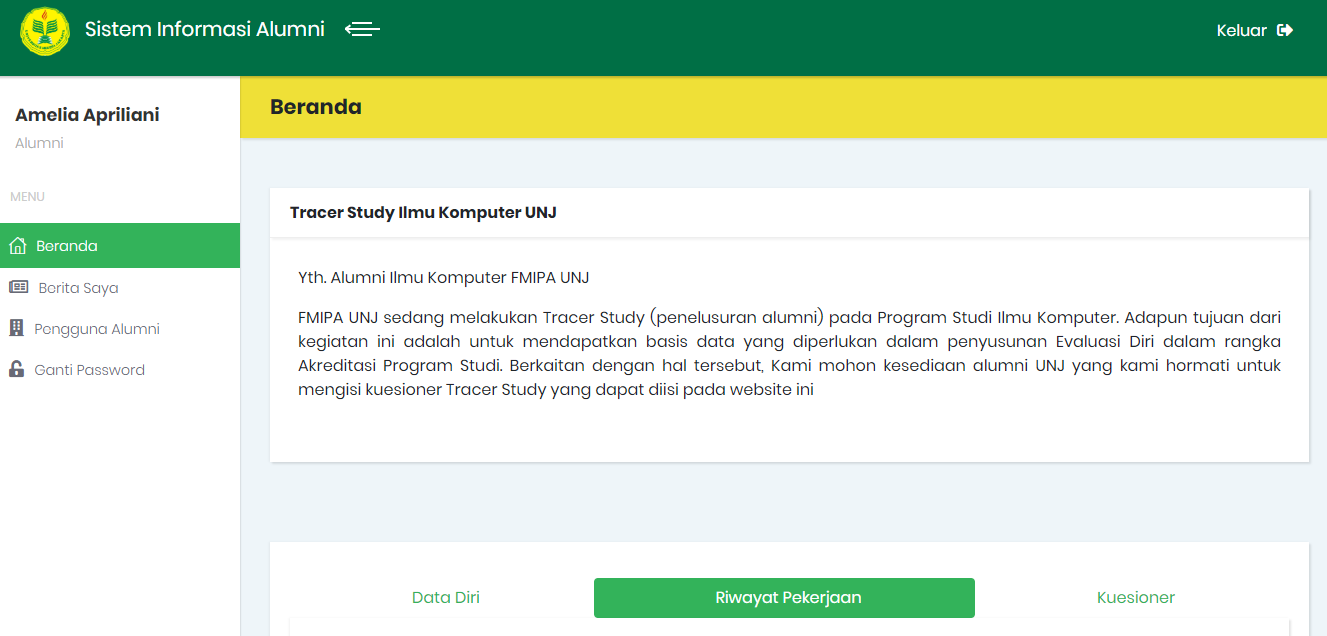
\includegraphics[width=14cm,height=7cm]{gambar/tampilan/alumni_beranda}
	\caption{Tampilan Halaman Beranda pada Alumni }
	\label{ui_alumniBeranda}
\end{figure}

Selanjutnya halaman alumni, setelah alumni melakukan \textit{login} sistem akan menampilkan halaman beranda alumni yang dapat dilihat pada Gambar 3.33. Beranda alumni berisi kata pengantar \textit{tracer study} yang dapat disunting oleh admin serta pengisian data \textit{tracer study} yang terdiri dari data diri, pekerjaan, dan kuesioner.  

\begin{figure}[H]
	\centering
	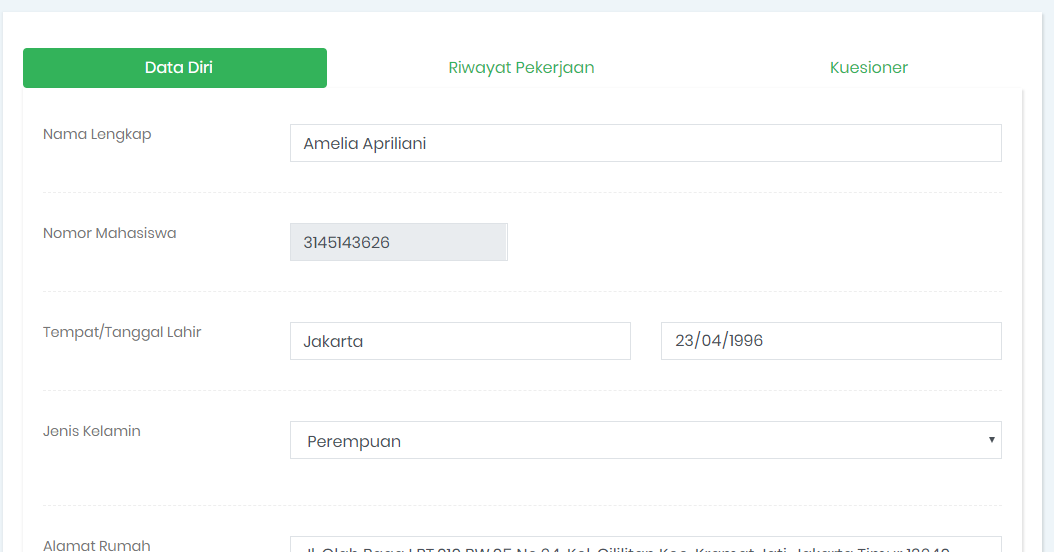
\includegraphics[width=14cm,height=7cm]{gambar/tampilan/alumni_profil}
	\caption{Tampilan Halaman Data Diri pada Alumni }
	\label{ui_alumniProfil}
\end{figure}

\begin{figure}[H]
	\centering
	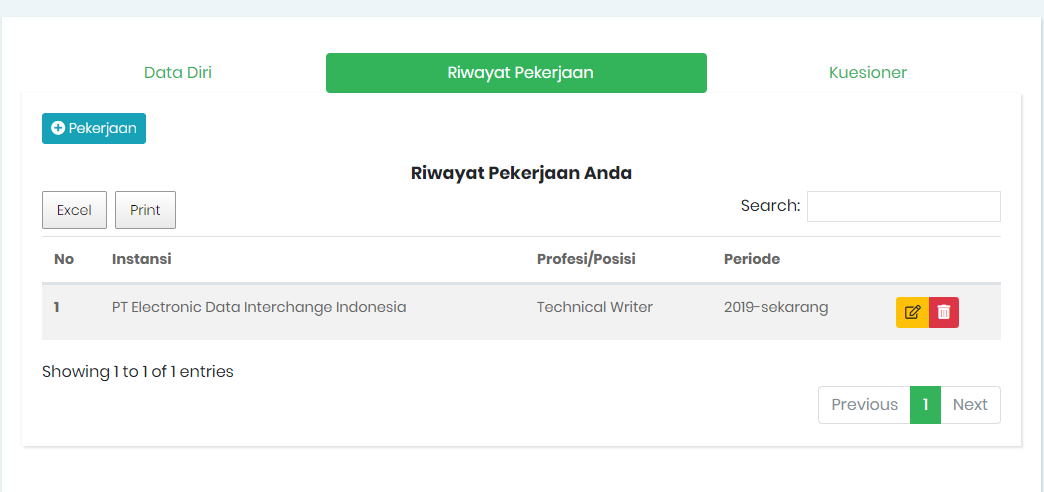
\includegraphics[width=14cm,height=7cm]{gambar/tampilan/alumni_pekerjaan}
	\caption{Tampilan Halaman Form Riwayat Pekerjaan pada Alumni }
	\label{ui_alumniInputPekerjaan}
\end{figure}

Gambar 3.34 adalah tampilan untuk melengkapi data diri alumni. Sedangkan gambar 3.35 merupakan tampilan form untuk memasukan data riwayat pekerjaan alumni

\begin{figure}[H]
	\centering
	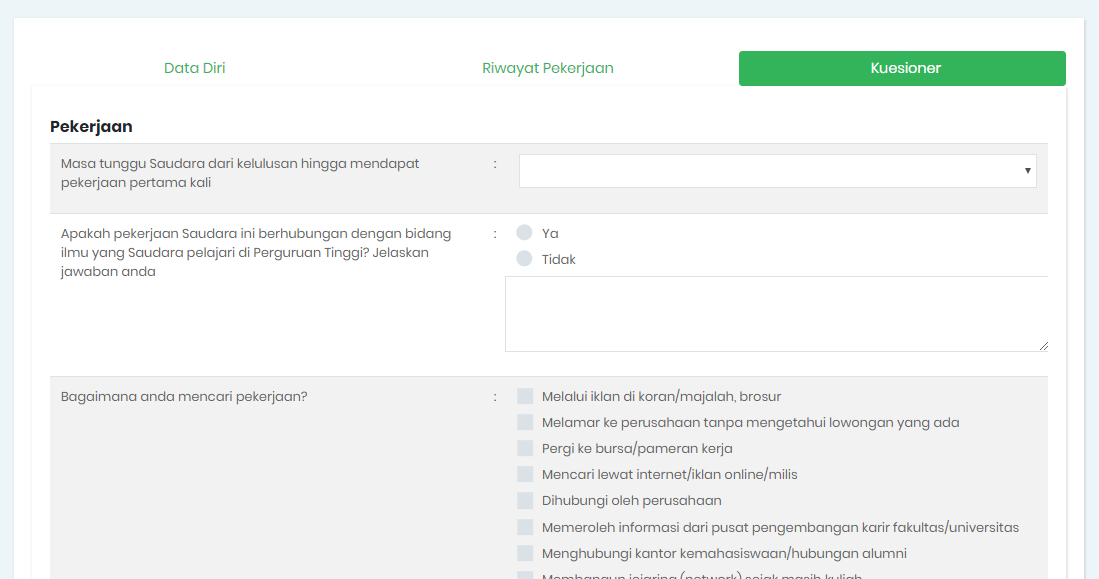
\includegraphics[width=14cm,height=7cm]{gambar/tampilan/alumni_kuesioner}
	\caption{Tampilan Halaman Kuesioner pada Alumni }
	\label{ui_alumniKuesioner}
\end{figure}

Gambar 3.36 adalah tampilan halaman mengisi kuesioner untuk alumni. Semua jenis kuesioner ditampilkan dalam satu halaman. Halaman kuesioner ini menyediakan pertanyaan isian, pilihan, ganda atau dapat memilih lebih dari satu jawaban, dan pertanyaan dengan skala penilaian.


\begin{figure}[H]
	\centering
	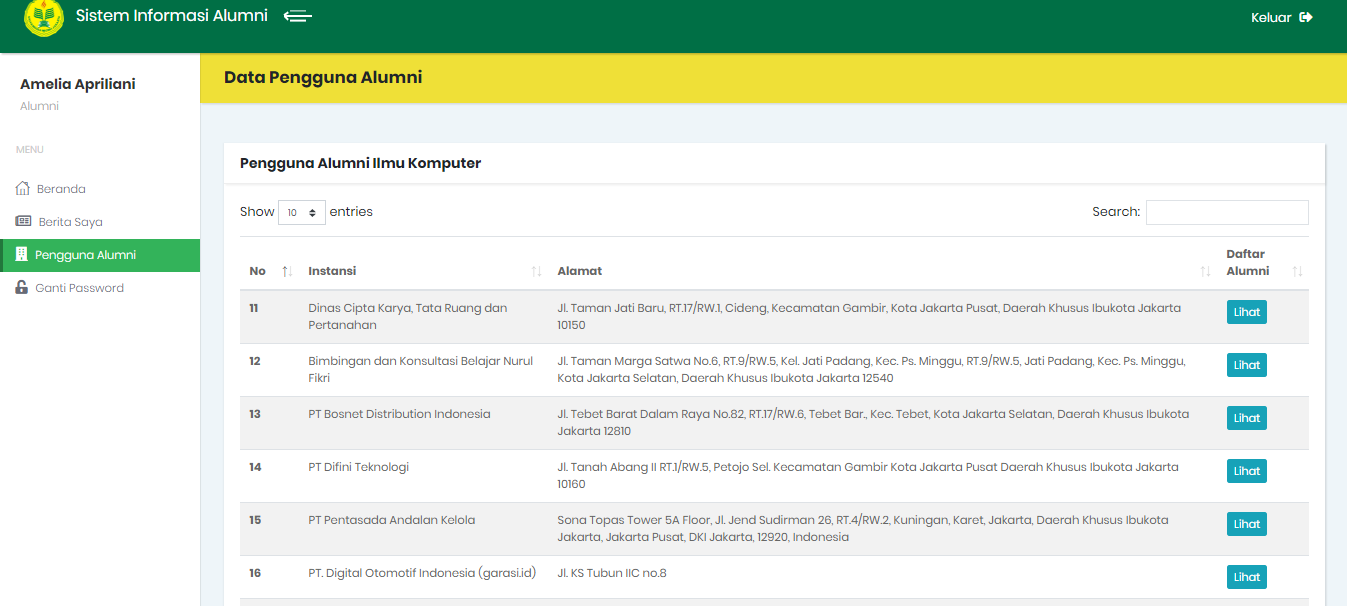
\includegraphics[width=14cm,height=7cm]{gambar/tampilan/alumni_daftarPengguna}
	\caption{Tampilan Halaman Daftar Pengguna pada Alumni }
	\label{ui_alumniDaftarPengguna}
\end{figure}

\begin{figure}[H]
	\centering
	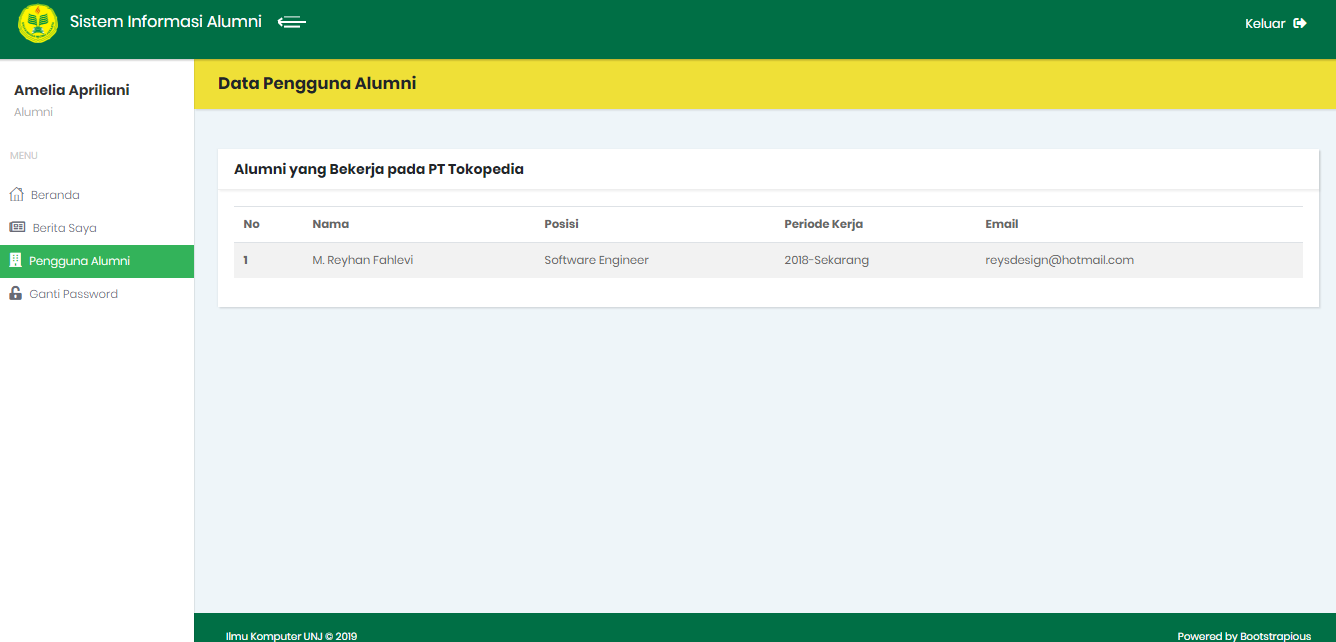
\includegraphics[width=14cm,height=7cm]{gambar/tampilan/alumni_alumniPengguna}
	\caption{Tampilan Halaman Daftar Pengguna pada Alumni }
	\label{ui_alumniPengguna}
\end{figure}

Pada pengembangan sistem ini menyediakan fasilitas untuk berbagi informasi antar alumni dapat dilihat pada Gambar 3.37 dan Gambar 3.38. Gambar 3.37 merupakan halaman daftar pengguna alumni pada alumni. Pada halaman ini alumni dapat melihat daftar pengguna alumni dari prodi Ilmu Komputer. Jika alumni memilih tombol lihat pada kolom daftar alumni, sistem akan menampilkan halaman daftar alumni yang bekerja pada pengguna alumni terkait seperti pada Gambar 3.38. 

\begin{figure}[H]
	\centering
	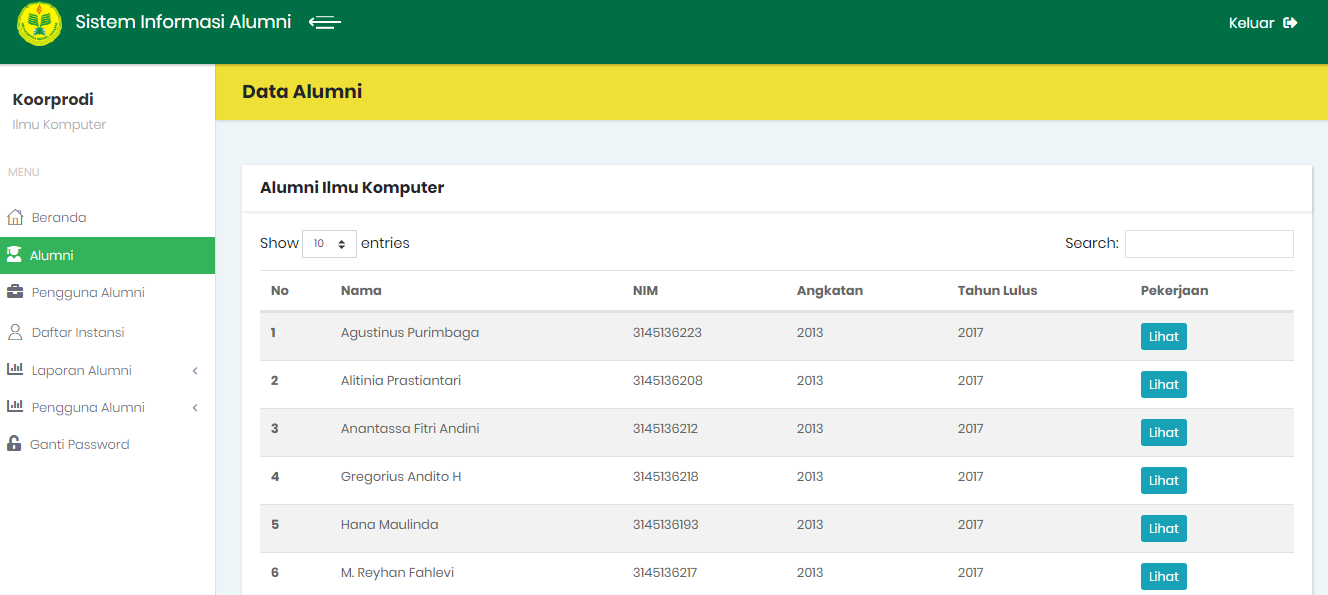
\includegraphics[width=14cm,height=7cm]{gambar/tampilan/koorprodi_daftarAlumni}
	\caption{Tampilan Halaman Daftar Alumni pada Koorprodi }
	\label{ui_koorprodiDaftarAlumni}
\end{figure}

Selanjutnya halaman untuk koorprodi. Halaman koorprodi dapat dilihat pada Gambar 3.39. Halaman koorprodi menyediakan menu untuk melihat data alumni beserta pekerjaannya, menu untuk melihat daftar pengguna alumni, menu untuk melihat daftar instansi beserta skala instansi dan menu untuk halaman laporan hasil \textit{tracer study}. 

\begin{figure}[H]
	\centering
	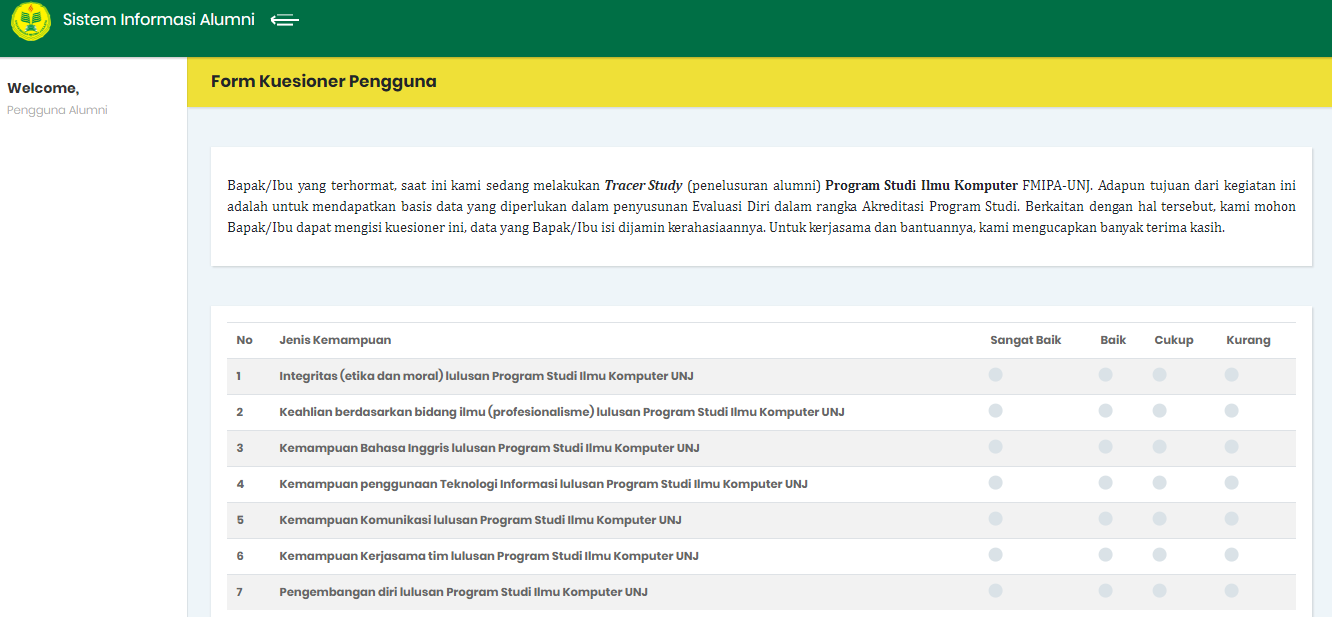
\includegraphics[width=14cm,height=7cm]{gambar/tampilan/penggunaAlumni_kuesioner}
	\caption{Tampilan Halaman Kuesioner untuk Pengguna Alumni}
	\label{ui_penggunaAlumniKuesioner}
\end{figure}

Gambar 3.40 merupakan halaman kuesioner yang diperuntukkan untuk pengguna alumni. Halaman ini akan muncul setelah pengguna alumni mengklik \textit{link} kuesioner yang dikirimkan admin melalui \textit{email}. 

\begin{figure}[H]
	\centering
	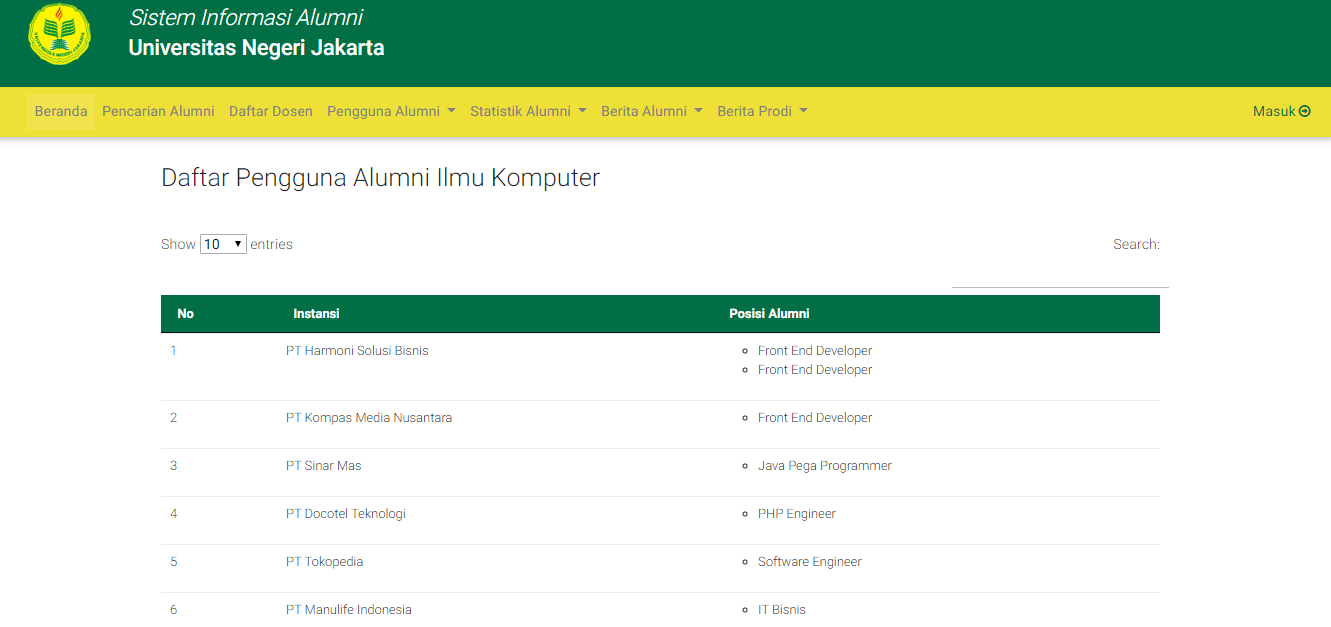
\includegraphics[width=14cm,height=7cm]{gambar/tampilan/pengunjung_daftarPengguna}
	\caption{Tampilan Halaman Daftar Pengguna Alumni untuk Pengunjung}
	\label{ui_pengunjungDaftarPengguna}
\end{figure}

\begin{figure}[H]
	\centering
	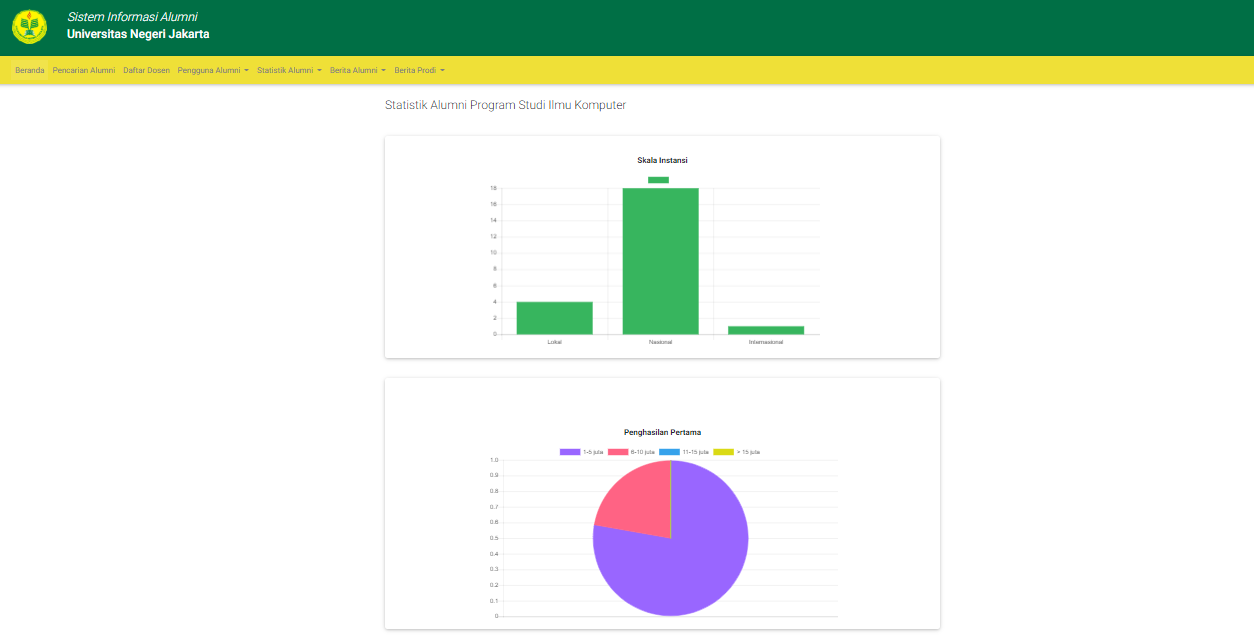
\includegraphics[width=14cm,height=7cm]{gambar/tampilan/pengunjung_statistik}
	\caption{Tampilan Halaman Statistik Alumni untuk Pengunjung}
	\label{ui_pengunjungStatistik}
\end{figure}

Selanjutnya adalah tampilan halaman yang dapat dilihat oleh pengunjung \textit{website} tanpa \textit{login}, yaitu terdapat halaman daftar pengguna alumni yang dapat dilihat pada Gambar 3.41 dan halaman statistik alumni yang dapat dilihat pada Gambar 3.42. Halaman daftar pengguna alumni berisi instansi-instansi tempat alumni bekerja beserta posisi pekerjaan alumni pada instansi terkait. Sedangkan halaman statistik alumni berisi beberapa hasil \textit{tracer study} yang dapat dilihat pengunjung.

\subsection{Implementasi Sistem (\textit{Back End})}
Dalam pengimplementasian semua fungsi yang berada dalam sistem digunakan bahasa pemrograman PHP kemudian menggunakan \textit{framework codeIgniter} untuk memudahkan dalam mengimplementasikan arsitektur MVC. Dengan arsitektur MVC proses pengkodean dibagi menjadi tiga bagian, yaitu Model untuk menyimpan fungsi yang berhubungan dengan \textit{database}, kemudian View untuk menampilkan informasi yang direpresentasikan kepada pengguna, dan Controller yang menjembatani antara Model dan View. Berikut merupakan sampel pemrograman terdiri dari \textit{Model}, \textit{View}, dan \textit{Controller}.

\begin{figure}[H]
	\centering
	\includegraphics[width=14cm,height=7cm]{gambar/source_code/c_alumni}
	\caption{Struktur Pemrograman \textit{Controller}}
	\label{sc_cAlumni}
\end{figure}

\begin{figure}[H]
	\centering
	\includegraphics[width=14cm,height=7cm]{gambar/source_code/m_alumni}
	\caption{Struktur Pemrograman \textit{Model}}
	\label{sc_mAlumni}
\end{figure}

\begin{figure}[H]
	\centering
	\includegraphics[width=14cm,height=7cm]{gambar/source_code/v_alumni}
	\caption{Struktur Pemrograman \textit{View}}
	\label{sc_vAlumni}
\end{figure}


%!TEX root = ./template-skripsi.tex
%-------------------------------------------------------------------------------
%                            	BAB IV
%               		UJI COBA DAN HASIL UJI COBA
%-------------------------------------------------------------------------------

\chapter{UJI COBA DAN HASIL UJI COBA}

\section{Uji Coba}
Pada bagian ini akan dijelaskan mengenai pengujian Sistem Informasi \textit{Tracer Study} Program Studi Ilmu Komputer yang telah dikembangkan. Sesuai dengan tahapan SDLC \textit{spiral model} setelah tahapan konstruksi atau pengembangan akan dilanjutkan ke tahapan evaluasi atau pengujian. Tahapan ini bertujuan untuk memastikan sistem yang telah dibuat dapat bekerja sesuai dengan kebutuhan, memperoleh umpan balik dari pengguna, dan menemukan kesalahan atau \textit{bugs} pada sistem. 

Uji coba pada sistem dilakukan tehadap satu responden ahli untuk uji keseluruhan sistem, satu reponden admin, satu responden koorprodi, 15 responden alumni, dan 5 responden pengguna alumni. Setiap responden akan melakukan pengujian terhadap sistem berdasarkan peran masing-masing responden. Uji coba yang dilakukan menggunakan kuesioner Pengujian Penerimaan Pengguna atau yang disebut dengan UAT (\textit{User Acceptance Test}). Langkah-langkah pengujian Sistem Informasi \textit{Tracer Study} Prodi Ilmu Komputer adalah sebagai berikut. 

\begin{enumerate}
	\item Admin mengelola (menambah, menyunting, menghapus) data alumni. 
	\item Admin menyunting kata pengantar untuk beranda alumni
	\item Admin membuat kuesioner untuk alumni dan pengguna alumni
	\item Alumni menyunting profil atau data diri
	\item Alumni mengelola  (menambah, menyunting, menghapus) riwayat pekerjaan. 
	\item Alumni mengisi kuesioner yang dibuat admin
	\item Admin mengelola (menambah, menyunting, menghapus) data pengguna alumni.
	\item Pengguna alumni mengisi kuesioner yang dibuat admin
	\item Admin melihat laporan hasil \textit{tracer study}
	\item Koorprodi melihat data alumni dan pengguna alumni
	\item Koorprodi melihat laporan hasil \textit{tracer study}
\end{enumerate}

Pengujian pada sistem ini terdiri dari dua, yaitu pengujian fungsional dan kebergunaan atau \textit{usability}. Pengujian fungsional berfokus pada fungsionalitas perangkat lunak yang dikembangkan. Sedangkan pengujian kebergunaan dilakukan untuk mengetahui tanggapan pengguna terhadap sistem seberapa efisien dan efektif sistem yang dikembangkan dalam membantu pengguna memenuhi kebutuhannya. Berikut adalah komponen-komponen yang akan diuji pada Sistem Informasi \textit{Tracer Study} Prodi Ilmu Komputer:

\begin{enumerate}
	\item Admin
	\begin{itemize}
		\item Mengelola (menambah, menyunting, menghapus) data alumni
		\item Mengelola (menambah, menyunting, menghapus) data pengguna alumni
		\item Menyunting kata pengantar \textit{tracer study}
		\item Membuat kuesioner alumni dan pengguna alumni
		\item Melihat laporan hasil \textit{tracer study}
	\end{itemize}
	\item Kooprodi
	\begin{itemize}
		\item Melihat data alumni
		\item Melihat data pengguna alumni
		\item Melihat laporan hasil \textit{tracer study}. 
	\end{itemize} 
	\item Alumni
	\begin{itemize}
		\item Menyunting data diri dan mengelola riwayat pekerjaan
		\item Mengisi form kuesioner \textit{tracer study}
		\item Melihat daftar pengguna alumni beserta alumni yang bekerja
	\end{itemize} 
	\item Pengguna Alumni
	 \begin{itemize}
	 	\item Mengisi form kuesioner pengguna alumni
	 \end{itemize}
\end{enumerate}
Dari semua komponen penilaian tersebut untuk pengujian fungsional dilakukan
dengan dua pilihan yaitu :
\begin{enumerate}
	\item S  : Setuju
	\item TS : Tidak Setuju
\end{enumerate}
Sedangkan untuk pengujian kebergunaan (\textit{usability}) dilakukan menggunakan skala \textit{likert}. Skala \textit{likert} merupakan 
suatu skala penilaian yang menyajikan pilihan skala dengan nilai pada setiap skala untuk mengukur tingkat persetujuan terhadap sesuatu \cite{Maryuliana}.  Skala yang digunakan dengan nilai 1 sampai 5 dengan perincian sebagai berikut :
\begin{itemize}
	\item 1 : Sangat Tidak Setuju
	\item 2 : Tidak Setuju
	\item 3 : Cukup
	\item 4 : Setuju
	\item 5 : Sangat Setuju
\end{itemize}

Berdasarkan nilai yang didapatkan dari pengguna saat pengujian, angka tersebut akan dikalkulasikan sesuai dengan sistem penilaian berikut :

\begin{itemize}
	\item Nilai total
	
	Nilai total merupakan jumlah keseluruhan nilai/skor yang didapat pada setiap pertanyaan atau dapat ditulis menjadi:
	
	$Nilai$ $Total = (jumlah \times skor SS) + (jumlah \times skor S) + (jumlah \times skor C) + (jumlah \times skor TS) + (jumlah \times skor STS)$ 
	
	\item Persentase Kelayakan
	
	Presentase kelayakan atau persentase nilai rata-rata yang didapatkan dari nilai total dibagi skor yang diharapkan. Skor yang diharapkan didapat dari skor maksimal yang dikalikan dengan jumlah responden. Skor maksimal adalah nilai maksimal dari skala \textit{likert} dikalikan dengan jumlah pertanyaan. Perhitungan tersebut dapat ditulis menjadi :
	
	$Persentase$ $Kelayakan (\%) = $ $\frac{Nilai Total}{Skor Diharapkan}$ $\times 100\%$

\end{itemize}

Persentase kelayakan yang didapatkan akan dibandingkan dengan skor pada skala \textit{likert}. Berikut model skala \textit{likert} lima skala :
\begin{enumerate}
	\item Sangat Kurang Sesuai = 0\%-20\%
	\item Kurang Sesuai = 21\%-40\%
	\item Cukup Sesuai = 41\%-60\%
	\item Sesuai = 61\%-80\%
	\item Sangat Sesuai = 81\%-100\%
\end{enumerate}

\section{Hasil Percobaan}
Berdasarkan percobaan yang dilakukan terhadap 1 admin, 1 koorprodi, 15 alumni, dan 5 pengguna alumni, didapatkan hasil percobaan sebagai berikut :

\subsection{Pengujian oleh Admin}
Pengujian untuk \textit{user} admin dilakukan oleh seorang responden yang bernama Bapak Alfisyahrizqa selaku staf admin prodi Ilmu Komputer pada tanggal 8 Januari 2020. Penilaian yang diberikan seputar fungsionalitas dan kebergunaan dari halaman \textit{user} admin pada sistem \textit{tracer study} Ilmu Komputer

\begin{enumerate}
	\item Uji Coba Fungsional
	
	Tabel 4.1 adalah hasil uji fungsional pada admin \textit{tracer study} :
	
	\begin{table}[H]
		\centering
		\caption{Hasil Uji Fungsional pada \textit{user} Admin}
		\includegraphics[width=10cm,height=9cm]{gambar/UAT/f_admin}
		\label{f_admin}
	\end{table}

Berdasarkan hasil uji coba fungsional yang dilakukan, keseluruhan fitur \textit{user} admin pada  sistem informasi \textit{tracer study} prodi Ilmu Komputer dapat berjalan dengan baik dan sesuai dengan yang diharapkan.
	
	\item Uji Coba Kebergunaan
	
	Berikut merupakan daftar pertanyaan uji \textit{usability} pada Admin:
	
	\begin{table}[H]
		\centering
		\caption{Daftar Pertanyaan Uji \textit{Usability} pada Admin}
		\includegraphics[width=11cm,height=10cm]{gambar/UAT/u_admin}
		\label{u_admin}
	\end{table}
	
	Berikut merupakan hasil uji kebergunaan pada admin \textit{tracer study} yang dapat dilihat pada tabel berikut:
	
	\begin{table}[H]
		\centering
		\caption{Hasil uji \textit{usability} pada Admin}
		\includegraphics[width=12cm,height=7cm]{gambar/UAT/hasil_u_admin}
		\label{h_u_admin}
	\end{table}
	
	$Nilai$ $Total = (0 \times 1) + (0 \times 1) + (0 \times 3) + (9 \times 4) + (0 \times 5) = 36$
	
	$Persentase$ $kelayakan (\%) = \frac{36}{45} $ $\times 100\%$ = 80\%
	
	Berdasarkan hasil uji coba kebergunaan yang telah dilakukan, didapatkan persentase kelayakan senilai \textbf{80\%}. Maka dapat dikatakan halaman pada \textit{user} admin mendapatkan predikat sesuai untuk aspek kebergunaan sistem. Dengan catatan data pada sistem di-\textit{update} dengan data terbaru.
	
\end{enumerate}

\subsection{Pengujian oleh Koorprodi}
Pengujian untuk \textit{user} koorprodi dilakukan oleh seorang responden yang bernama Ibu Ir. Fariani Hermin I, M.T. selaku koorprodi Ilmu Komputer pada tanggal 8 Januari 2020. Penilaian yang diberikan terkait fungsionalitas dan kebergunaan dari halaman \textit{user} koorprodi pada sistem tracer study Ilmu Komputer.

\begin{enumerate}
	\item Uji Coba Fungsional
	
	Tabel 4.4 adalah hasil uji fungsional pada koorprodi :
	
	\begin{table}[H]
		\centering
		\caption{Hasil Uji Fungsional pada Koorprodi}
		\includegraphics[width=11cm,height=7cm]{gambar/UAT/f_koorprodi}
		\label{f_koorprodi}
	\end{table}
	
	%lihat lg hasil real nya/jelasin
	Berdasarkan hasil uji coba fungsional yang dilakukan, sistem informasi
	\textit{tracer study} prodi Ilmu Komputer dapat berjalan dengan baik dan sesuai dengan yang dibutuhkan. Koorprodi Ilmu Komputer dapat melihat data alumni dan pengguna alumni, dapat melihat laporan hasil \textit{tracer study}, dan \textit{export} data \textit{tracer}.
	
	\item Uji Coba Kebergunaan
	
	Berikut merupakan daftar pertanyaan uji \textit{usability} pada Koorprodi:

	\begin{table}[H]
		\centering
		\caption{Daftar Pertanyaan Uji \textit{Usability} pada Koorprodi}
		\includegraphics[width=11cm,height=7cm]{gambar/UAT/u_koorprodi}
		\label{u_koorprodi}
	\end{table}
	
	Berikut merupakan hasil uji \textit{usability} pada koorprodi yang dapat dilihat pada tabel berikut:
	
	\begin{table}[H]
		\centering
		\caption{Hasil Uji \textit{Usability} pada Koorprodi}
		\includegraphics[width=11cm,height=8cm]{gambar/UAT/hasil_u_koorprodi}
		\label{h_u_koorprodi}
	\end{table}
	
	$Nilai$ $Total = (0 \times 1) + (0 \times 2) + (0 \times 3) + (0 \times 4) + (6 \times 5) = 30$
	
	$Persentase$ $kelayakan (\%) = \frac{30}{30} $ $\times 100\%$ = 100\%

	Berdasarkan hasil uji coba kebergunaan yang telah dilakukan pada \textit{user} koorprodi, didapatkan persentase kelayakan senilai \textbf{100\%}. Maka dapat dikatakan halaman pada \textit{user} koorprodi mendapatkan predikat sangat sesuai untuk aspek kebergunaan sistem.
	
\end{enumerate}

\subsection{Pengujian oleh Alumni}
	\textit{User Acceptance Test} pada \textit{user} Alumni dilakukan oleh 15 responden alumni prodi Ilmu Komputer UNJ terdiri dari angkatan 2013 sampai 2015. Penilaian yang diberikan mengenai fungsionalitas dan kebergunaan dari halaman \textit{user} alumni pada sistem \textit{tracer study} Ilmu Komputer.

\begin{enumerate}
	\item Uji Coba Fungsional
	
	Tabel 4.7 adalah hasil uji fungsional pada alumni :
	
	\begin{table}[H]
		\centering
		\caption{Hasil Uji Fungsional pada Alumni}
		\includegraphics[width=11cm,height=8cm]{gambar/UAT/f_alumni}
		\label{f_alumni}
	\end{table}
	
	%lihat lg hasil real nya/jelasin
	Berdasarkan hasil uji coba fungsional yang dilakukan pada 15 responden alumni, didapatkan jumlah total jawaban 102 dari maksimal nilai 105, maka persentase jawaban adalah \textbf{97.14\%} sehingga dapat dikatakan fitur-fitur pada halaman alumni dapat berjalan dengan baik dan sesuai dengan yang diharapkan. 
	
	\item Uji Coba Kebergunaan
	
	Berikut merupakan daftar pertanyaan uji \textit{usability} pada Alumni:
	
	\begin{table}[H]
		\centering
		\caption{Daftar Pertanyaan Uji \textit{Usability} pada Alumni}
		\includegraphics[width=11cm,height=8cm]{gambar/UAT/u_alumni}
		\label{u_alumni}
	\end{table}
	
	Berikut merupakan hasil uji \textit{usability} pada alumni yang dapat dilihat pada tabel berikut:
	
	\begin{table}[H]
		\centering
		
		\includegraphics[width=12cm,height=8cm]{gambar/UAT/hasil_u_alumni}
		\label{h_u_alumni}
	\end{table}
	
	$Nilai$ $Total = (0 \times 1) + (5 \times 2) + (16 \times 3) + (51 \times 4) + (33 \times 5) = 427$
		
	$Persentase$ $kelayakan (\%) = \frac{427}{525} $ $\times 100\%$ = 81.33\%
	
	Berdasarkan hasil uji coba kebergunaan yang telah dilakukan pada 15 responden alumni, didapatkan persentase kelayakan senilai \textbf{81.33\%}. Maka dapat dikatakan halaman pada \textit{user} alumni mendapatkan predikat sangat sesuai untuk aspek kebergunaan sistem.
	
\end{enumerate}

\subsection{Pengujian oleh Pengguna Alumni}
\textit{User Acceptance Test} pada \textit{user} Pengguna Alumni dilakukan oleh 5 responden yang merupakan atasan dari alumni di instansi tempat alumni bekerja. Penilaian yang diberikan mengenai fungsionalitas dan kebergunaan dari halaman \textit{user} pengguna alumni pada sistem \textit{tracer study} Ilmu Komputer.

\begin{enumerate}
	\item Uji Coba Fungsional
	
	Tabel 4.9 adalah hasil uji fungsional pada pengguna alumni :
	
	\begin{table}[H]
		\centering
		\includegraphics[width=11cm,height=3cm]{gambar/UAT/f_pengguna}
		\caption{Hasil Uji Fungsional pada Pengguna Alumni}
		\label{f_pengguna}
	\end{table}
	
	%lihat lg hasil real nya/jelasin
	Berdasarkan hasil uji coba fungsional yang dilakukan pada \textit{user} pengguna alumni, sistem informasi
	\textit{tracer study} prodi Ilmu Komputer dapat berjalan dengan baik dan sesuai dengan yang diharapkan. Pengguna alumni dapat mengisi kuesioner secara \textit{online}.
	
	\item Uji Coba Kebergunaan
	
	Tabel 4.10 merupakan daftar pertanyaan dari uji kebergunaan/\textit{usability} pada pengguna alumni:
	
	\begin{table}[H]
		\centering
		\includegraphics[width=12cm,height=3cm]{gambar/UAT/u_pengguna}
		\caption{Daftar Pertanyaan Uji \textit{Usability} pada Pengguna Alumni}
		\label{u_pengguna}
	\end{table}
	
	Berikut merupakan hasil uji \textit{usability} pada pengguna alumni yang dapat dilihat pada tabel berikut:
	
	\begin{table}[H]
		\centering
		\includegraphics[width=10cm,height=5cm]{gambar/UAT/hasil_u_pengguna}
		\caption{Hasil Uji \textit{Usability} pada Pengguna Alumni}
		\label{h_u_pengguna}
	\end{table}
	
	
	$Nilai$ $Total = (0 \times 1) + (0 \times 2) + (3 \times 3) + (8 \times 4) + (4 \times 5) = 61$
	
	$Persentase$ $kelayakan (\%) = \frac{61}{75} $ $\times 100\%$ = 81.33\%
	
	Berdasarkan hasil uji coba kebergunaan yang telah dilakukan pada 5 responden pengguna alumni, didapatkan persentase kelayakan senilai \textbf{81.33\%}. Maka dapat dikatakan halaman pada \textit{user} pengguna alumni mendapatkan predikat sangat sesuai untuk aspek kebergunaan sistem.
	
\end{enumerate}

%\subsection{Pengujian oleh Ahli}

%Pengujian sistem oleh ahli dilakukan pada keseluruhan sistem. Uji fungsional maupun uji kebergunaan dilakukan pada setiap \textit{user}, yaitu admin, koorprodi, alumni, dan pengguna alumni. Berdasarkan hasil uji coba fungsional yang dilakukan ahli, fungsionalitas sistem pada setiap \textit{user} dapat berjalan dengan baik dan sesuai dengan yang diharapkan. %catatan hasil real
%Hasil uji coba fungsional oleh ahli dapat dilihat sebagai berikut :

%tabel semua fungsional

%Hasil uji coba kualitas yang dilakukan ahli, sistem informasi\textit{tracer study} ilmu komputer dapat berjalan dengan baik dan sudah cukup sesuai dengan kebutuhan. %catatan hasil real
%Hasil uji coba kualitas oleh ahli dapat dilihat sebagai berikut

%tabel semua kualitas

\subsection{Hasil Pengujian Keseluruhan Sistem}
Berdasarkan hasil pengujian fungsional dan kebergunaan (\textit{usability}) Sistem Informasi \textit{Tracer Study} Program Studi Ilmu Komputer pada semua \textit{user},didapatkan bahwa fitur-fitur yang terdapat pada sistem dapat berjalan dengan baik. Selain itu, didapatkan persentase kelayakan sebagai berikut:
 
\begin{itemize}
	\item Halaman \textit{user} Admin : 80\%
	\item Halaman \textit{user} Koorprodi : 100\%
	\item Halaman \textit{user} Alumni : 81.33\%
	\item Halaman \textit{user} Pengguna Alumni : 81.33\%
\end{itemize}

	Dari persentase masing-masing \textit{user} kemudian dihitung total persentase kelayakan yang merupakan rata-rata dari nilai persentase kelayakan semua user, dapat dilihat sebagai berikut:
	
	$Total Persentase Kelayakan (\%) = \frac{80\%+ 100\% + 81.33\%+ 81.33\%}{4} = 85.66\% $
	
	Berdasarkan perhitungan tersebut didapatkan total persentase kelayakan senilai \textbf{85.66\%} berada pada rentang tafsiran 81\%-100\%,  maka dapat dikatakan bahwa nilai kebergunaan pada keseluruhan sistem mendapatkan predikat sangat sesuai. 

% Baris ini digunakan untuk membantu dalam melakukan sitasi
% Karena diapit dengan comment, maka baris ini akan diabaikan
% oleh compiler LaTeX.
\begin{comment}
\bibliography{daftar-pustaka}
\end{comment}

%!TEX root = ./template-skripsi.tex
%-------------------------------------------------------------------------------
%                            	BAB V
%               		KESIMPULAN DAN SARAN
%-------------------------------------------------------------------------------

\chapter{KESIMPULAN DAN SARAN}

\section{Kesimpulan}
Berdasarkan hasil implementasi dan pengujian program ini, maka didapat kesimpulan sebagai berikut:

\begin{enumerate}
	\item Pengembangan Sistem Informasi \textit{Tracer Study} Program Studi Ilmu Komputer berdasarkan dari analisis dan evaluasi perbandingan fitur sistem \textit{tracer study} yang telah tersedia, yaitu Sistem Informasi \textit{Tracer Study} Universitas Negeri Jakarta dan Sistem \textit{Tracer Study} Dikti. Selain itu, melalui pengumpulan data yang diperoleh dari analisis kebutuhan prodi Ilmu Komputer. 
	
	\item Fitur terbaru yang terdapat pada Sistem Informasi \textit{Tracer Study} Program Studi Ilmu Komputer adalah kuesioner dan \textit{feedback} dari pengguna alumni, hak akses koorprodi, \textit{open access} pengunjung, informasi pekerjaan antar alumni, halaman mengelola riwayat pekerjaan alumni, dan admin dapat menyunting kata pengantar \textit{tracer study}. 
	
	\item Proses pengembangan Sistem Informasi \textit{Tracer Study} Program Studi Ilmu Komputer menggunakan metode pengembangan perangkat lunak \textit{System Development Life Cycle} dengan \textit{Spiral Model} yang memiliki beberapa tahapan, yaitu pengumpulan dan analisis kebutuhan, perancangan atau desain, konstruksi atau pengkodean, dan pengujian atau evaluasi.
	
	\item Sistem Informasi \textit{Tracer Study} Program Studi Ilmu Komputer dikembangkan dengan bahasa pemrograman PHP dengan bantuan \textit{framework Codeigniter}. %Berdasarkan hasi user acceptence test dengan 	menggunakan metode black box, didapatkan rata-rata nilai 4,29 untuk responden alumni dan 4,70 untuk responden admin program studi dalam skala 5. Maka dapat disimpulkan bahwa sistem informasi yang dikembangkan sudah sesuai dan dapat berjalan dengan baik.
	
	\item Berdasarkan hasil \textit{User Acceptance Test} pada pengujian fungsional didapatkan bahwa fitur-fitur yang terdapat pada Sistem Informasi \textit{Tracer Study} Program Studi Ilmu Komputer dapat berjalan dengan baik dan sesuai kebutuhan.
	
	\item Berdasarkan hasil \textit{User Acceptance Test} pada pengujian kebergunaan (\textit{usability}), didapatkan total persentase kelayakan dari keseluruhan sistem adalah 85.66\%. Nilai tersebut terdapat pada skor skala \textit{likert} 81\%-100\%, maka nilai kebergunaan Sistem Informasi \textit{Tracer Study} Program Studi Ilmu Komputer mendapat predikat sangat sesuai.
	
	\item  Sistem Informasi \textit{Tracer Study} Program Studi Ilmu Komputer dikembangkan untuk dapat dimanfaatkan pihak prodi terkait pengelolaan data alumni, menghasilkan informasi hasil \textit{tracer study} yang dibutuhkan prodi untuk mengingkatkan kualitas pendidikannya dan memenuhi kebutuhan akreditasi. Selain itu, ditujukan untuk masyarakat agar dapat lebih mengenal lulusan prodi Ilmu Komputer

\end{enumerate}


\section{Saran}
Adapun beberapa saran untuk penelitian selanjutnya adalah:
\begin{enumerate}
	
	\item Meningkatkan ruang lingkup penelitian menjadi rumpun ataupun fakultas. 
	
	\item Menambahkan halaman yang menampilkan status pengisian kuesioner. 
	
	\item Mengembangkan Sistem Informasi \textit{Tracer Study} Ilmu Komputer berbasis \textit{Mobile}. 
		
\end{enumerate}


% Baris ini digunakan untuk membantu dalam melakukan sitasi
% Karena diapit dengan comment, maka baris ini akan diabaikan
% oleh compiler LaTeX.
\begin{comment}
\bibliography{daftar-pustaka}
\end{comment}

\addcontentsline{toc}{chapter}{DAFTAR PUSTAKA}


%-----------------------------------------------------------------
%Disini akhir masukan Bab
%-----------------------------------------------------------------


%-----------------------------------------------------------------
% Disini awal masukan untuk Daftar Pustaka
% - Daftar pustaka diambil dari file .bib yang ada pada folder ini
%   juga.
% - Untuk memudahkan dalam memanajemen dan menggenerate file .bib
%   gunakan reference manager seperti Mendeley, Zotero, EndNote,
%   dll.
%-----------------------------------------------------------------
%\bibliography{IEEEabrv,daftar-pustaka}
\begin{thebibliography}{99}
	
\bibitem{Rifqi} Alim, R. S.(2019). Perancangan dan Implementasi Sistem Informasi Penelusuran Alumni (Tracer Study) [Skripsi]. Jakarta: Universitas Negeri Jakarta.

\bibitem{Elisabet} Anggraeni, E. Y., Irviani, R. (2017). Pengantar Sistem Informasi. Yogyakarta: ANDI.

\bibitem{Rosa} S., Rosa A., Shalahuddin, M. (2014). Rekayasa Perangkat Lunak Struktur dan Berorientasi Objek. Bandung: Informatika.

\bibitem{Azis} Azis, M. F. (2005). \textit{Object Oriented Programming} dengan PHP 5. Jakarta: Elex Media Komputindo

\bibitem{Sebastian} Boell, S. K., Cecez-Kecmanovic, D. (2015). What is an Information System?. \textit{Hawaii International Conference on System Sciences}.

\bibitem{DoroEdi} Edi, D., Betshani, S. (2009). Analisis Data dengan Menggunakan ERD dan Model Konseptual Data \textit{Warehouse}. \textit{Jurnal Informatika}, 5(1).

\bibitem{Nuryake} Fajaryati, N., Priyanto, Sukardiyono, T., Wiji, A. D., Pambudi, S., Destiana, B. (2015). Studi Penelusuran (\textit{Tracer Study}) Terhadap Alumni. \textit{Jurnal Electronics, Informatics, and Vocational Education (ELINVO)}, 1(1).

\bibitem{BPAFMIPA} FMIPA Universitas Negeri Jakarta. (2015). Pedoman Akademik 2015/2016 Fakultas Matematika dan Ilmu Pengetahuan Alam (FMIPA) Universitas Negeri Jakarta. Jakarta: Universitas Negeri Jakarta.

\bibitem{Fridayanthie} Fridayanthie, E. W., Mahdiati, T. (2016). Rancang Bangun Sistem Informasi Permintaan Atk Berbasis Intranet. \textit{Jurnal Khatulistiwa Informatika}, 2(4).

\bibitem{Ghozaly} Ghozaly, A., Nurcahyawati, V., Suhandiah, S. (2016). Rancang Bangun Aplikasi \textit{Tracer Study} Berbasis Web Pada Stikes Yayasan Rs. Dr. Soetomo Surabaya. \textit{Jurnal Sistem Informasi dan Komputer Akuntansi}, 5(6).

\bibitem{Wellem} Hartomo, K. D., Wellem, T., Sanjaya, A. D. (2009). Implementasi \textit{Model View Controller} dan \textit{Object Relational Mapping} pada Content Management System Sistem Informasi Keuangan. \textit{Jurnal Teknologi Informasi}, 6(1).

\bibitem{Haviluddin} Haviluddin. (2011). Memahami Penggunaan UML (Unified Modelling Language). \textit{Jurnal Informatika Mulawarman}, 6(1).

\bibitem{AdeHendini} Hendini, A. (2016). Pemodelan UML Sistem Informasi Monitoring Penjualan Dan Stok. \textit{Jurnal Khatulistiwa Informatika}, 4(2).

\bibitem{Fariani} Hermin, F. (2017). Desain Sistem Informasi Alumni (SILUNI) Berbasis \textit{Website}. Jakarta: Universitas Negeri Jakarta.

\bibitem{AriefHidayat} Hidayat, A., Surarso, B. (2012). Penerapan Arsitektur Model View Controller (MVC) dalam Rancang Bangun Sistem Kuis \textit{Online} Adaptif. \textit{Seminar Nasional Teknologi Informasi dan Komunikasi 2012 (SENTIKA 2012)}.

\bibitem{BorangIlkom} Ilmu Komputer FMIPA UNJ. (2017). Borang Akreditasi Program Studi Ilmu Komputer. Jakarta: Universitas Negeri Jakarta.

\bibitem{Martono} Martono, K. T. (2018). Rancang Bangun Sistem Informasi Produksi Ayam Petelur Dengan Menggunakan \textit{Framework Codeigniter}. \textit{Jurnal Sistem Komputer}, 8(1).

\bibitem{Maryuliana} Maryuliana, Subroto, M. I., Chairul, S. F. (2016). Sistem Informasi Angket Pengukuran Skala Kebutuhan Materi Pembelajaran Tambahan sebagai Pendukung Pengambilan Keputusan di Sekolah Menengah Atas Menggunakan \textit{Skala Likert}. \textit{Jurnal Transistor Elektro dan Informatika}, 1(2).

\bibitem{Muslihudin} Muslihudin, M., Oktafianto. (2016). Analisis dan Perancangan Sistem Informasi. Yogyakarta: ANDI.

\bibitem{EkoNursubiyantoro} Nursubiyantoro, E., Puryani. (2016). Perancangan Sistem Penulusuran Alumni (\textit{Tracer Study}) Berbasis Web. \textit{Jurnal Optimasi Sistem Industri (OPSI)}, 9(2).

\bibitem{Pressman} Pressman, R. S. (2002). Rekayasa Perangkat Lunak. LN Harnaningrum, penerjemah: Yogyakarta: Andi.  dari: Software Engineering, a Practitioner's Approach. McGraw Hill Company, Inc.

\bibitem{Made} Raharja, I. S., SN, A. (2012). Perbandingan Proses Pengembangan Perangkat Lunak. \textit{Seminar Nasional Informatika 2012 (semnasIF 2012)}.

\bibitem{ExploringTS} Renny, Chandra, R., Ruhana, S., Sarjono, M. W. (2013). Exploring Tracer Study Service in Career Center. \textit{International Journal of Computer Science and Information Security (IJCSIS)}, 11(3).

\bibitem{RistekdiktiPanduan} Ristekdikti. (2018). Panduan Program Bantuan Pengembangan Layanan Pusat Karir Lanjutan/Tracer Study 2019. Diambil dari http://pkts.belmawa.ristekdikti.go.id/upload/1548740521Panduan-Bantuan-PKL-2019.pdf

\bibitem{RistekdiktiWeb} Ristekdikti. (2018). Tentang \textit{Tracer Study}. Diambil dari http://pkts.belmawa.ristekdikti.go.id/index.php/site/about

\bibitem{Mohit} Sharma, M. K. (2017). A Study of SDLC to Develop Well Engineered Software. \textit{International Journal of Advanced Research in Computer Science}, 8(3).

\bibitem{Sulianta} Sulianta, F., Juju, D. (2010). Data Mining. Jakarta: Elex Media Komputindo.

\bibitem{Edhy} Sutanta, E. (2004). Sistem Basis Data. Yogyakarta: Graha Ilmu.

\bibitem{Robi} Yanto, R. (2016). Manajemen Basis Data Menggunakan MySQL. Yogyakarta: Deepublish.

	
		
	
\end{thebibliography}

%-----------------------------------------------------------------
%Disini akhir masukan Daftar Pustaka
%-----------------------------------------------------------------
\addcontentsline{toc}{chapter}{LAMPIRAN}
\appendix 
\chapter{Perbandingan Fitur Sistem \textit{Tracer Study}}

\begin{figure}[H]
	\centering
	\includegraphics[width=1.0\textwidth]{gambar/tabelFitur}
	\label{tabelFitur}
\end{figure}

\begin{figure}[H]
	\centering
	\includegraphics[width=1.0\textwidth]{gambar/tabelFitur2}
	\label{tabelFitur2}
\end{figure}

\chapter{Perbandingan Kuesioner Sistem \textit{Tracer Study}}

\begin{figure}[H]
	\centering
	\includegraphics[width=1.0\textwidth]{gambar/tabelKuesioner}
	\label{tabelKuesioner}
\end{figure}

\begin{figure}[H]
	\centering
	\includegraphics[width=1.0\textwidth]{gambar/tabelKuesioner2}
	\label{tabelKuesioner2}
\end{figure}

\begin{figure}[H]
	\centering
	\includegraphics[width=1.0\textwidth]{gambar/tabelKuesioner3}
	\label{tabelKuesioner3}
\end{figure}

\chapter{Analisis Kebutuhan Sistem dengan Pihak Prodi Ilmu Komputer}

\begin{enumerate}
	\item Kapan diadakannya kegiatan tracer study pada prodi Ilmu Komputer?
	Kegiatan tracer study telah dilakukan sejak prodi ini memiliki lulusan pertama pada semester 2016/2017.
	\item Bagaimana proses pelaksanaan tracer study pada prodi Ilmu Komputer?
	Pelaksanaan tracer study tersebut dilakukan melalui pengiriman kuesioner melalui pos, e-mail dan media sosial seperti whatsapp
	\item Apakah terdapat kendala selama proses tracer study berlangsung?
	Bentuk pelaksanaan tersebut dirasa kurang efektif karena dapat membutuhkan waktu lama terhadap respon alumni
	\item Apakah saat ini sudah tersedia sistem tracer study yang dapat diakses secara online?
	Saat ini terdapat sistem tracer study milik WR3 yang juga memiliki layanan di tingkat prodi. Karena sistem yang disediakan bersifat umum untuk semua prodi terdapat beberapa kebutuhan dari prodi Ilkom yang belum bisa dipenuhi sistem tersebut seperti belum ada pengisian kuesioner oleh pengguna lulusan/alumni.  Selain itu, juga terdapat sistem tracer study milik Dikti namun untuk tingkat perguruan tinggi. 
	\item Mengapa diperlukan kuesioner untuk pengguna alumni?
	Penelitian terhadap pengguna diperlukan untuk mengetahui bagaimana penilaian pengguna terhadap kompetensi lulusan dan kurikulum yang berjalan apakah sudah mencukupi dan relevan dengan kebutuhan dunia kerja saat ini. 
	\item Jika akan dilakukan pengembangan sistem tracer study dikhususkan untuk prodi Ilmu Komputer, fasilitas apa yang diharapkan dari pengembangan sistem ini?
	\begin{itemize}
		\item Selain kuesioner untuk alumni juga disediakan fitur pengisian kuesioner secara online untuk pengguna alumni
		\item Koorprodi membutuhkan akses ke sistem untuk mengakses data tracer yang diperlukan bagi akreditasi maupun penjaminan mutu internal
		\item Disediakan open access bagi pengunjung untuk dapat melihat beberapa hasil tracer study seperti yang terdapat pada sistem tracer study Dikti. 
		\item Bandingkan sistem tracer study UNJ dan Dikti, ambil fitur yang sekiranya dapat bermanfaat untuk prodi. 
	\end{itemize}	
\end{enumerate}
\vspace{0.8cm}

\begin{tabular}{p{7.5cm}c}
	&Jakarta, April 2019\\
	&\\
	&\\
	&\\
	&\textbf{Ir. Fariani Hermin Indiyah, M.T}
\end{tabular}

\chapter{Sampel Kode \textit{Controller} Alumni pada Admin}

\begin{verbatim}

<?php
defined('BASEPATH') OR exit('No direct script access allowed');

class Alumni extends CI_Controller {
function __construct(){
parent::__construct();
if($_SESSION["logged_in"] != 'login') {
redirect(base_url("login"));
}

$this->load->model('m_alumni');
$this->load->model('m_master');
$this->load->model('m_pengguna');
$this->load->library(array('PHPExcel','PHPExcel/IOFactory'));

}

public function index()
{
$prodiID = $this->session->userdata('prodiID');
$data = array(
'role' => $this->session->userdata('role'),
'userID' => $this->session->userdata('userID'),
'prodiID' => $prodiID,
'alumni' => $this->m_alumni->getAlumni($prodiID),
);
$this->load->view('element/head');
$this->load->view('element/header');
$this->load->view('element/navbar', $data);
$this->load->view('admin/v_dataAlumni', $data);
$this->load->view('element/footer');
}

function exeAddAlumni()
{

$userID = 'ALU'.$this->input->post('nim');
$cek = $this->m_alumni->cekAlumni($this->input->post('nim'));

if($cek->num_rows() > 0){
$this->session->set_flashdata("gagalAddAlumni", '<div><div class="alert alert-danger" id="alert" align="center">Gagal menambahkan! Akun alumni sudah terdaftar</div></div>');
} else {

$data_user = array(
'userID' => $userID,
'username' => $this->input->post('nim'),
'password' => $this->input->post('nim'),
'prodiID' => $this->session->userdata('prodiID'),
'role' => 'alumni'
);
$this->m_master->inputData($data_user,'user');

$data_alumni = array(
'nama' => $this->input->post('nama'),
'nim' => $this->input->post('nim'),
'userID' => $userID,
'jenis_kelamin' => $this->input->post('jenis_kelamin'),
'tahun_masuk' => $this->input->post('tahun_masuk'),
'tahun_lulus' => $this->input->post('tahun_lulus'),
'prodiID' => $this->session->userdata('prodiID'),
);

$this->m_master->inputData($data_alumni,'alumni');

$this->session->set_flashdata("suksesAddAlumni", '<div><div class="alert alert-success" id="alert" align="center">Akun alumni berhasil ditambahkan!</div></div>');
}

redirect('admin/Alumni');
}

public function editProfil($id)
{
$data = array(
'role' => $this->session->userdata('role'),
'userID' => $this->session->userdata('userID'),
'prodiID' => $this->session->userdata('prodiID'),
'profil' => $this->m_alumni->getAlumniByID($id)
);
$this->load->view('element/head');
$this->load->view('element/header');
$this->load->view('element/navbar', $data);
$this->load->view('admin/v_editProfilAlumni', $data);
$this->load->view('element/footer');
}

function exeEditProfil()
{

$data_user = array(
'username' => $this->input->post('nim')
);
$id = $this->input->post('id');
$where = array('id' => $this->input->post('userID'));
$this->m_master->updateData($where,$data_user,'user');

$data_alumni = array(
'nama' => $this->input->post('nama'),
'nim' => $this->input->post('nim'),
'jenis_kelamin' => $this->input->post('jenis_kelamin'),
'tahun_masuk' => $this->input->post('tahun_masuk'),
'tahun_lulus' => $this->input->post('tahun_lulus'),
'ipk' => $this->input->post('ipk'),
'toefl' => $this->input->post('toefl'),
'alamat' => $this->input->post('alamat'),
'tempat_lahir' => $this->input->post('tempat_lahir'),
'tanggal_lahir' => $this->input->post('tanggal_lahir'),
'email' => $this->input->post('email'),
'no_telepon' => $this->input->post('no_telepon'),
);

$where = array('id' => $this->input->post('id'));
$this->m_master->updateData($where,$data_alumni,'alumni');

$this->session->set_flashdata("pesan", '<div><div class="alert alert-success" id="alert" align="center">Edit data alumni sukses!</div></div>');
redirect('admin/Alumni/editProfil/'.$id);
}

function exeImport()
{
if ($_FILES['file']['name']) {
$fileName = time().$_FILES['file']['name'];

$config['upload_path'] = FCPATH .'/assets/upload/';
$config['file_name'] = $fileName;
$config['allowed_types'] = 'xls|xlsx|csv';
$config['max_size'] = 10000;

$this->load->library('upload');
$this->upload->initialize($config);

if(! $this->upload->do_upload('file') )
$this->upload->display_errors();

$media = $this->upload->data('file');
$inputFileName = $this->upload->data('full_path');

try {
$inputFileType = IOFactory::identify($inputFileName);
$objReader = IOFactory::createReader($inputFileType);
$objPHPExcel = $objReader->load($inputFileName);
} catch(Exception $e) {
die('Error loading file "'.pathinfo($inputFileName,PATHINFO_BASENAME).'": '.$e->getMessage());
}

$sheet = $objPHPExcel->getSheet(0);
$highestRow = $sheet->getHighestRow();
$highestColumn = $sheet->getHighestColumn();

for ($row = 2; $row <= $highestRow; $row++){                  //  Read a row of data into an array
$rowData = $sheet->rangeToArray('A' . $row . ':' . $highestColumn . $row, NULL, TRUE, FALSE);

$nim = $rowData[0][1];
$cek = $this->m_alumni->cekAlumni($nim);
if($cek->num_rows() < 1){
//tabel user
$data = array(
"userID"=> "ALU".$rowData[0][1],
"username"=> $rowData[0][1],
"password"=> $rowData[0][1],
"role"=> 'alumni',
"prodiID" => $this->session->userdata('prodiID')
);

$insert = $this->db->insert("user",$data);
//tabel alumni
$data = array(
"nim"=> $rowData[0][1],
"nama"=> $rowData[0][0],
"no_telepon" => $rowData[0][2],
"ipk" => $rowData[0][3],
"userID"=> "ALU".$rowData[0][1],
"jenis_kelamin"=> $rowData[0][4],
"tahun_masuk"=> $rowData[0][5],
"tahun_lulus"=> $rowData[0][6],
"prodiID" => $this->session->userdata('prodiID')
);
$insert = $this->db->insert("alumni",$data);
} /*else {
unlink($inputFileName);
}*/
if ($rowData[0][7] != NULL) {
//tabel instansi
$where = array('nama_instansi' => $rowData[0][7]);
$cek = $this->m_master->cekData("instansi",$where)->num_rows();
if ($cek == 0) {
$data = array(
"nama_instansi" => $rowData[0][7],
"prodiID" => $this->session->userdata('prodiID')
);
$insert = $this->db->insert("instansi",$data);
$id_instansi = $this->m_master->getInstansiByName($rowData[0][7])->id;
} else {
$id_instansi = $this->m_master->getInstansiByName($rowData[0][7])->id;
}

//tabel pekerjaan
$alumniID = $this->m_alumni->getAlumniByUserID("ALU".$rowData[0][1])->id;
$where = array( 'id_alumni' => $alumniID);
$cek = $this->m_master->cekData("pekerjaan",$where)->num_rows();
if ($cek == 0) {
$firstPekerjaan = 'yes';
} else {
$firstPekerjaan = 'no';
}

$gajiawal = str_replace(".","",$rowData[0][9]);
$data = array(
"posisi" => $rowData[0][8],
"gaji" => $gajiawal,
"id_alumni" => $alumniID,
'firstPekerjaan' => $firstPekerjaan,
'id_instansi'=> $id_instansi
);
$insert = $this->db->insert("pekerjaan",$data);
} // if instansi not null

}
$this->session->set_flashdata("suksesImpor", '<div><div class="alert alert-info" id="alert" align="center">Data alumni berhasil diimpor</div></div>');
redirect('admin/Alumni');
} else {
$this->session->set_flashdata("gagalImpor", '<div><div class="alert alert-danger" id="alert" align="center">File belum dimasukkan</div></div>');
redirect('admin/Alumni');
}
}

function deleteAlumni($id){
//hapus pekerjaan
$where = array(
'id_alumni' => $id
);
$this->m_master->deleteData($where,'pekerjaan');
//hapus akun di tabel user
$userID = $this->m_alumni->getAlumniByID($id)->userID;
$where = array(
'userID' => $userID
);
$this->m_master->deleteData($where,'user');
//hapus data di tabel alumni
$where = array(
'id' => $id
);
$this->m_master->deleteData($where,'alumni');

$where = array(
'respondenID' => $id
);
$this->m_master->deleteData($where,'notif_kuesioner');
redirect('admin/Alumni');
}


}

\end{verbatim}


\chapter{Sampel Kode \textit{Model} Alumni pada Admin}

\begin{verbatim}

<?php 

class M_alumni extends CI_Model{	

public function __construct()
{
parent::__construct();
//$this->db2 = $this->load->database('db_dua', TRUE);
}

function getAlumniByUserID($userid)
{
$this->db->select('*');
$this->db->where('userID',$userid);
$query = $this->db->get('alumni');
return $query->row();

}

function getAlumniByID($id)
{
$this->db->select('*');
$this->db->where('id',$id);
$query = $this->db->get('alumni');
return $query->row();

}

function getAlumni($prodiID)
{
$this->db->select('*');
$this->db->where('status', 'aktif');
$this->db->where('prodiID', $prodiID);
$this->db->order_by('id', 'DESC');
$query = $this->db->get('alumni');
if($query->num_rows()>0)
{
return $query->result();
} else{
return $query->result();
}

}


function getAlumniByProdi($prodiID)
{
$this->db->select('*');
$this->db->where('status', 'aktif');
$this->db->where('prodiID', $prodiID);
$this->db->order_by('nama', 'ASC');
$query = $this->db->get('alumni');
if($query->num_rows()>0)
{
return $query->result();
} else{
return $query->result();
}

}

public function cekAlumni($nim){
$this->db->where('nim', $nim);
return $this->db->get('alumni');
}

function getRiwayatByAlumniID($id)
{
$this->db->select('*');
$this->db->where('id_alumni', $id);
$this->db->order_by('id', 'ASC');
$query = $this->db->get('pekerjaan');
if($query->num_rows()>0)
{
return $query->result();
} else{
return $query->result();
}

}

function getAlumniPengguna($id)
{
$this->db->select('*');
$this->db->where('id_alumni', $id);
$this->db->order_by('id', 'ASC');
$query = $this->db->get('pekerjaan');
if($query->num_rows()>0)
{
return $query->result();
} else{
return $query->result();
}

}

function hapusAlumniPengguna($id_alumni,$id_pengguna){
$this->db->where($id_alumni);
$this->db->where($id_pengguna);
$this->db->delete('alumni_pengguna');
}

function getPekerjaanByAlumniID($id)
{
$this->db->select('*');
$this->db->where('id_alumni', $id);
$query = $this->db->get('pekerjaan');
if($query->num_rows()>0)
{
return $query->result();
} else{
return $query->result();
}

}

function getPekerjaanByID($id)
{
$this->db->select('*');
$this->db->where('id',$id);
$query = $this->db->get('pekerjaan');
return $query->row();
}

public function joinPekerjaanAlumniByProdiID($prodiID){
$this->db->select('
pekerjaan.id AS id_pekerjaan, pekerjaan.*, alumni.id AS id_alumni, alumni.*
');
$this->db->join('alumni', 'pekerjaan.id_alumni = alumni.id');
$this->db->from('pekerjaan');
$this->db->where('alumni.prodiID',$prodiID);
$this->db->where('pekerjaan.gaji !=',"");
$query = $this->db->get();
return $query->result();
}

}

\end{verbatim}

\chapter{Kuesioner \textit{User Acceptance Test} pada Admin}

\begin{figure}[H]
	\centering
	\includegraphics[width=15cm,height=18cm]{gambar/UAT/surat kuesioner}
	\label{surat_kuesioner}
\end{figure}

\begin{figure}[H]
	\centering
	\includegraphics[width=10cm,height=12cm]{gambar/UAT/surat kuesioner 2}
	\label{surat_kuesioner2}
\end{figure}

\begin{figure}[H]
	\centering
	\includegraphics[width=15cm,height=18cm]{gambar/UAT/kf_admin}
	\label{kf_admin}
\end{figure}

\begin{figure}[H]
	\centering
	\includegraphics[width=15cm,height=18cm]{gambar/UAT/ku_admin}
	\label{ku_admin}
\end{figure}


\chapter{Kuesioner \textit{User Acceptance Test} pada Koorprodi}

\begin{figure}[H]
	\centering
	\includegraphics[width=15cm,height=18cm]{gambar/UAT/surat kuesioner}
	\label{surat_kuesioner}
\end{figure}

\begin{figure}[H]
	\centering
	\includegraphics[width=10cm,height=12cm]{gambar/UAT/surat kuesioner 2}
	\label{surat_kuesioner2}
\end{figure}

\begin{figure}[H]
	\centering
	\includegraphics[width=15cm,height=18cm]{gambar/UAT/kf_koorprodi}
	\label{kf_koorprodi}
\end{figure}

\begin{figure}[H]
	\centering
	\includegraphics[width=15cm,height=18cm]{gambar/UAT/ku_koorprodi}
	\label{ku_koorprodi}
\end{figure}


\chapter{Kuesioner \textit{User Acceptance Test} pada Alumni}

\begin{figure}[H]
	\centering
	\includegraphics[width=15cm,height=18cm]{gambar/UAT/surat kuesioner}
	\label{surat_kuesioner}
\end{figure}

\begin{figure}[H]
	\centering
	\includegraphics[width=10cm,height=12cm]{gambar/UAT/surat kuesioner 2 alumni}
	\label{surat_kuesioner2}
\end{figure}

\begin{figure}[H]
	\centering
	\includegraphics[width=15cm,height=18cm]{gambar/UAT/kf_alumni}
	\label{kf_alumni}
\end{figure}

\begin{figure}[H]
	\centering
	\includegraphics[width=15cm,height=18cm]{gambar/UAT/ku_alumni}
	\label{ku_alumni}
\end{figure}



\chapter{Kuesioner \textit{User Acceptance Test} pada Pengguna Alumni}

\begin{figure}[H]
	\centering
	\includegraphics[width=15cm,height=18cm]{gambar/UAT/surat kuesioner}
	\label{surat_kuesioner}
\end{figure}

\begin{figure}[H]
	\centering
	\includegraphics[width=10cm,height=12cm]{gambar/UAT/surat kuesioner 2}
	\label{surat_kuesioner2}
\end{figure}

\begin{figure}[H]
	\centering
	\includegraphics[width=15cm,height=18cm]{gambar/UAT/kf_pengguna}
	\label{kf_pengguna}
\end{figure}

\begin{figure}[H]
	\centering
	\includegraphics[width=15cm,height=18cm]{gambar/UAT/ku_pengguna}
	\label{ku_pengguna}
\end{figure}


\chapter{Kuesioner \textit{User Acceptance Test} pada Pengguna Alumni}
\pagestyle{empty}
\chapter*{\centering \large DAFTAR RIWAYAT HIDUP}
\thispagestyle{empty}

\begin{wrapfigure}{l}{4cm}
	\vspace{-25pt}
	\begin{center}
		\includegraphics[width=0.27\textwidth]{gambar/pas-foto2}
	\end{center}
	\vspace{-80pt}
\end{wrapfigure}

\noindent \textbf{SAULIA KARINA.}  Lahir di Jakarta, 27 Juni 1997  Anak pertama dari pasangan Bapak Syarifudin dan Ibu Ana Yohana. Saat ini beralamatkan di Jl. Pisangan Baru I RT.006 RW.08 No.4, Kecamatan Matraman Jakarta Timur.

\vspace{0.5cm}
\noindent
\begin{center}
	\begin{flushright}
		\begin{tabular}{lcl}
			No. Ponsel	& :&  083843549167 \\
			Email	& :&  sauliakarina@gmail.com
		\end{tabular}
	\end{flushright}
\end{center}
\vspace{0.5cm}

\noindent \textbf{Riwayat Pendidikan} : Penulis mengawali pendidikan di TK Nurul Iman pada tahun 2002 - 2003, dan kemudian melanjutkan pendidikan di SDN Pisangan Baru 01 Pagi pada tahun 2003 - 2009. Setelah itu, penulis melanjutkan ke SMPN 7 Jakarta hingga tahun 2012. Kemudian melanjutkan ke SMAN 54 Jakarta pada tahun 2012-2015. Di Tahun 2015 penulis melanjutkan ke Universitas Negeri Jakarta (UNJ), Program Studi Ilmu Komputer, melalui jalur PENMABA. Di awal tahun 2020 (D, dd Februari 2020) penulis telah memperoleh gelar Sarjana Komputer (S.Kom), Program Studi Ilmu Komputer, Fakultas Matematika dan Ilmu Pengetahuan Alam, Universitas Negeri Jakarta.

\noindent \textbf{Riwayat Organisasi} : Selama di bangku perkuliahan, penulis aktif di Badan Eksekutif Mahasiswa Rumpun Matematika sebagai staff di Departemen Advokasi dan Keolahragaan kemudian melanjutkan di BEM FMIPA dengan departemen yang sama. Penulis juga berpartisipasi dalam kegiatan BINER (Be Innovative and Educated Researcher) yaitu kegiatan workshop dan seminar yang diadakan oleh DEFAULT, dimana penulis tergabung sebagai anggota merangkap Bendahara. 

\end{document}